\documentclass[../Thesis.tex]{subfiles}
\begin{document}
\section{Cài đặt server side open source Canvas LMS trên Google Cloud}
    Trong phần này, chúng ta sẽ trình bày quá trình cài đặt server side open source Canvas LMS trên nền tảng Google Cloud. Canvas LMS được xây dựng bằng ngôn ngữ Ruby và được triển khai trên máy chủ web.
    \subsection{Chuẩn bị môi trường}
    \begin{enumerate}
        \item Đăng ký tài khoản Google Cloud: Truy cập vào trang web của Google Cloud và tạo một tài khoản nếu bạn chưa có. Sau khi hoàn thành việc đăng ký, bạn sẽ được chuyển đến bảng điều khiển Google Cloud.
        \begin{figure}[ht!]
            \centering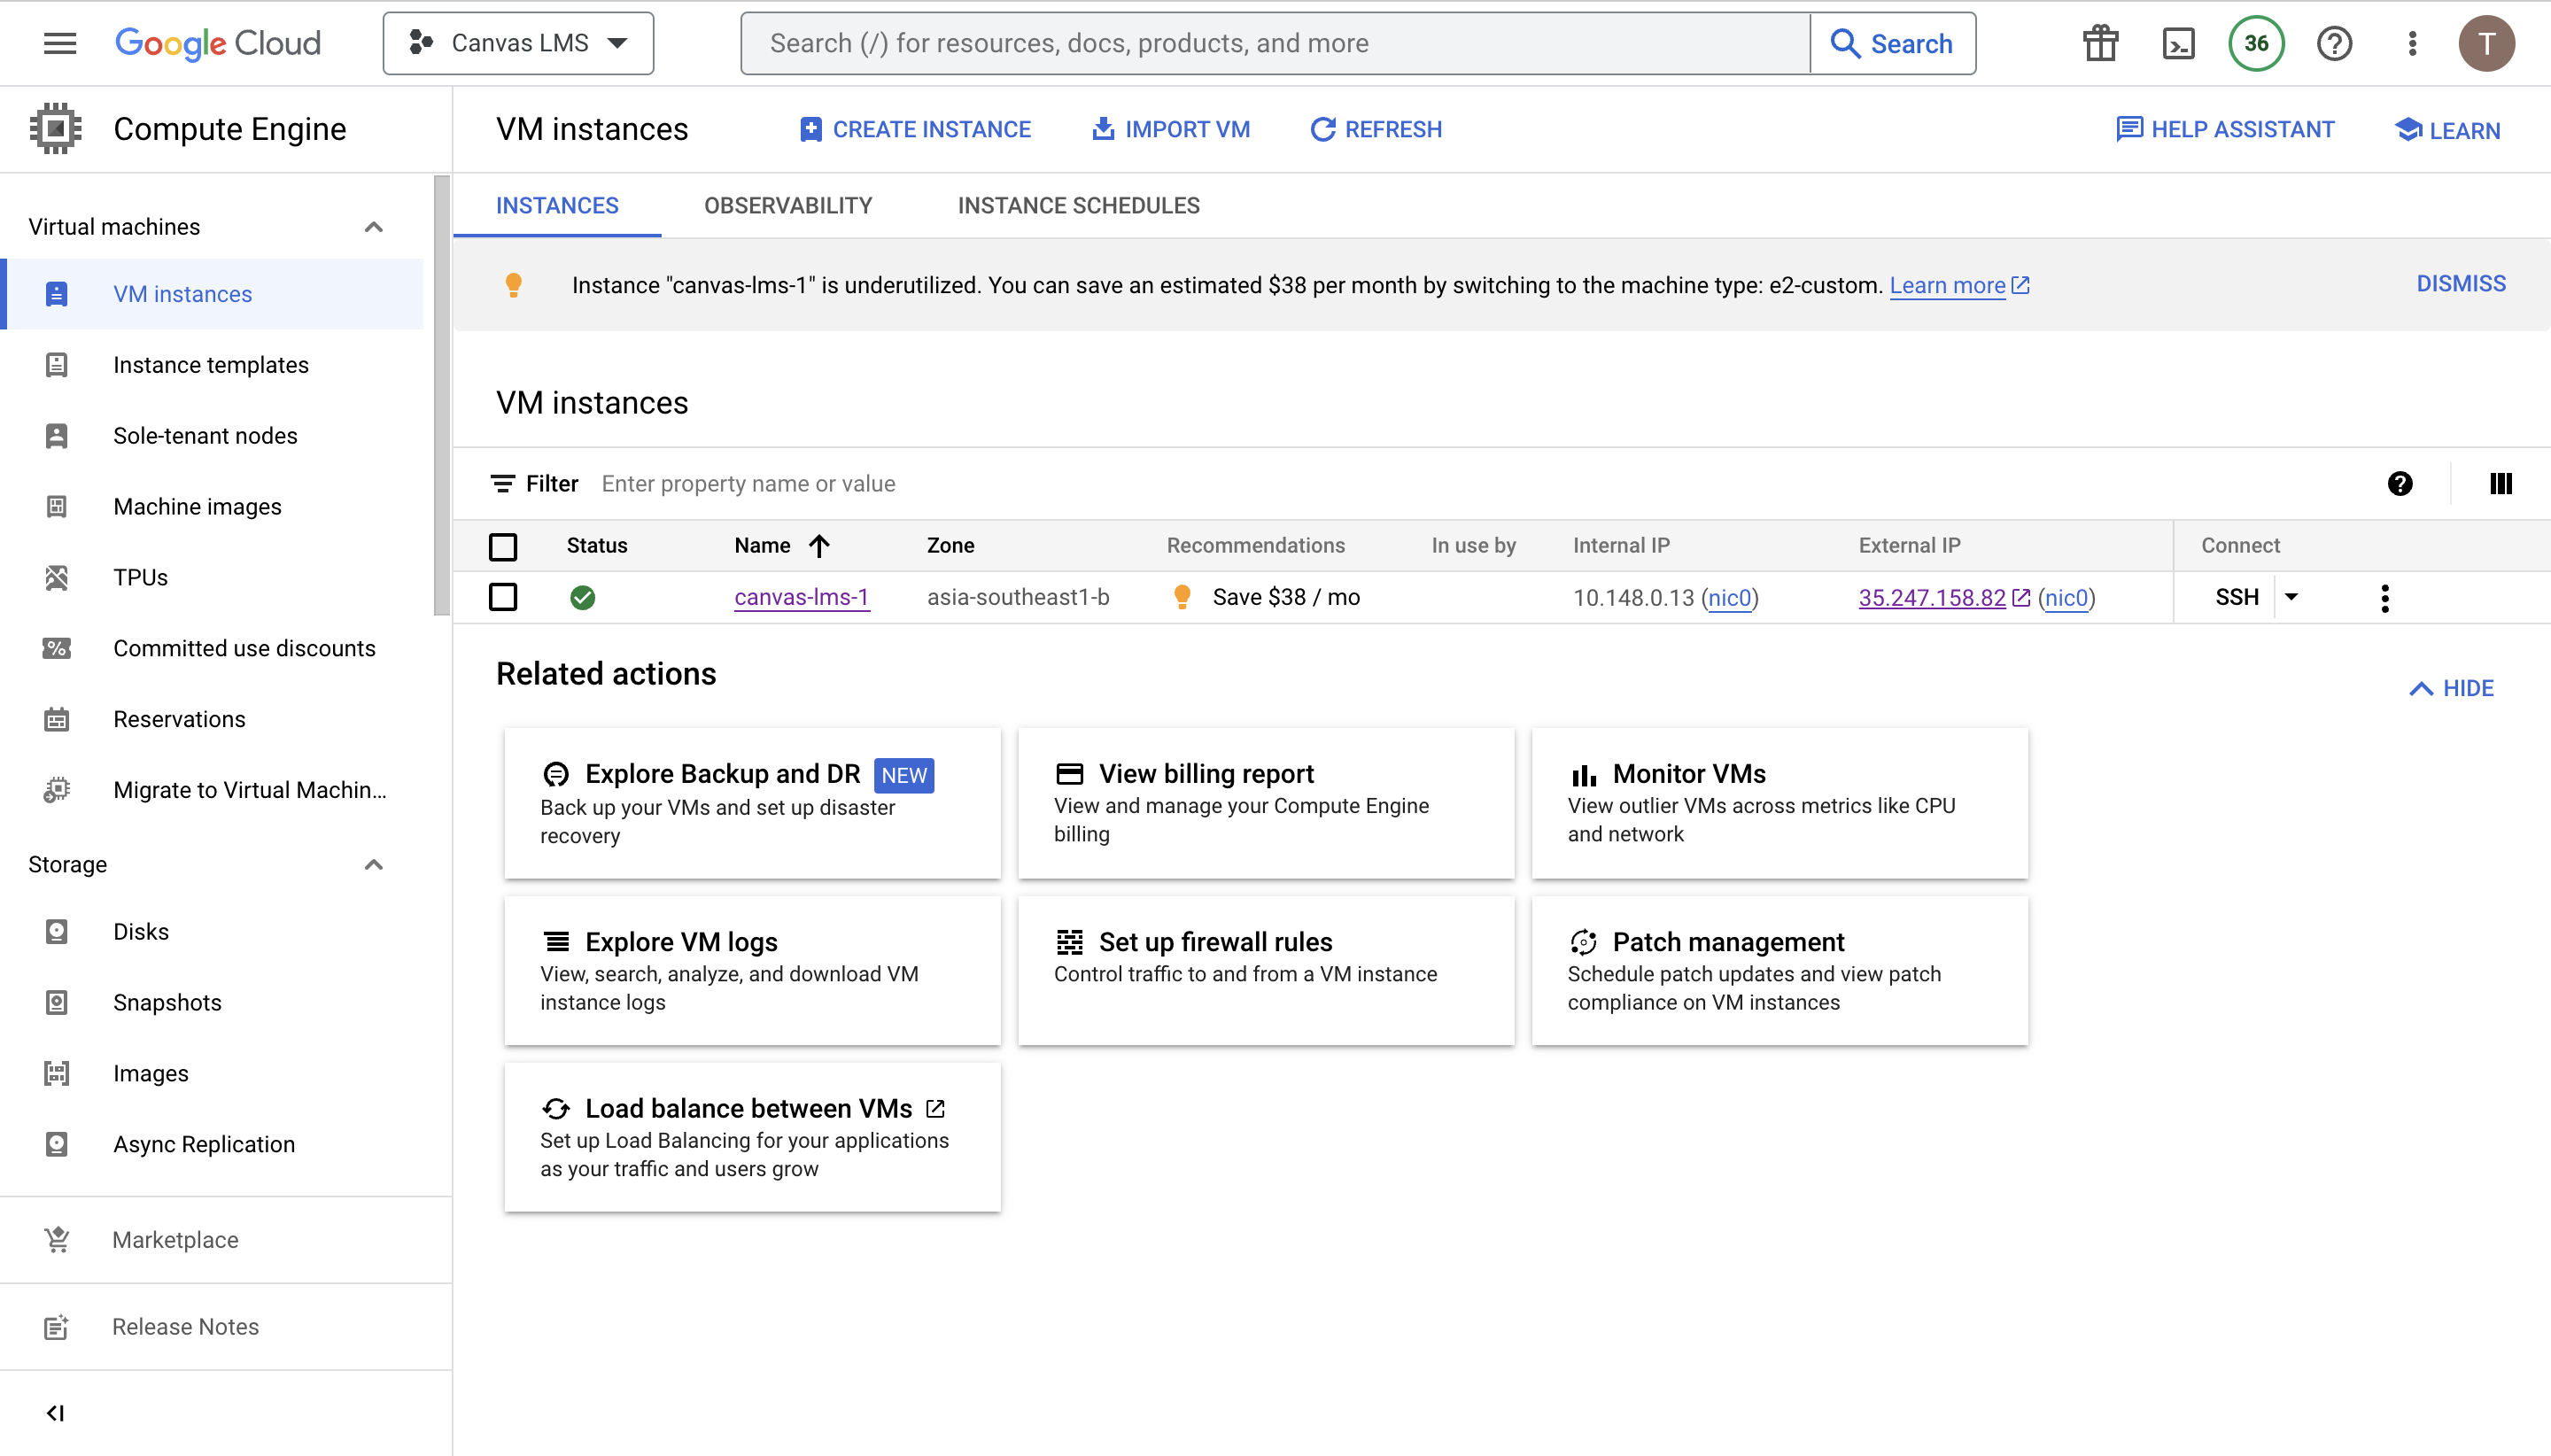
\includegraphics[width=300pt]{1-google-cloud-console}
            \caption{Màn hình Google Cloud Console}
            \label{fig:google-cloud-console}
        \end{figure}
        \item Tạo máy ảo: Trên bảng điều khiển Google Cloud, chúng ta sẽ thực hiện việc tạo một máy ảo để chạy Canvas LMS. Để tạo máy ảo, chúng ta nhấp vào mục "Compute Engine" trên bảng điều khiển. Tiếp theo, chọn "Máy ảo" và nhấp vào nút "Tạo máy ảo".

        Trong trang tạo máy ảo, bạn sẽ cần cung cấp các thông tin sau:
        \begin{itemize}
            \item Tên máy ảo: Đặt tên cho máy ảo của bạn để dễ nhận biết.
            \item Kích thước máy ảo: Chọn kích thước máy ảo phù hợp với yêu cầu của bạn, bao gồm số lượng bộ nhớ RAM và vCPU.
            \item Vùng địa lý: Chọn vùng địa lý gần với địa điểm của bạn để đảm bảo tốc độ truy cập nhanh nhất.
            \item Firewall: Cấu hình các quy tắc tường lửa cho phép truy cập vào máy ảo.
        \end{itemize}
        \begin{figure}[ht!]
            \centering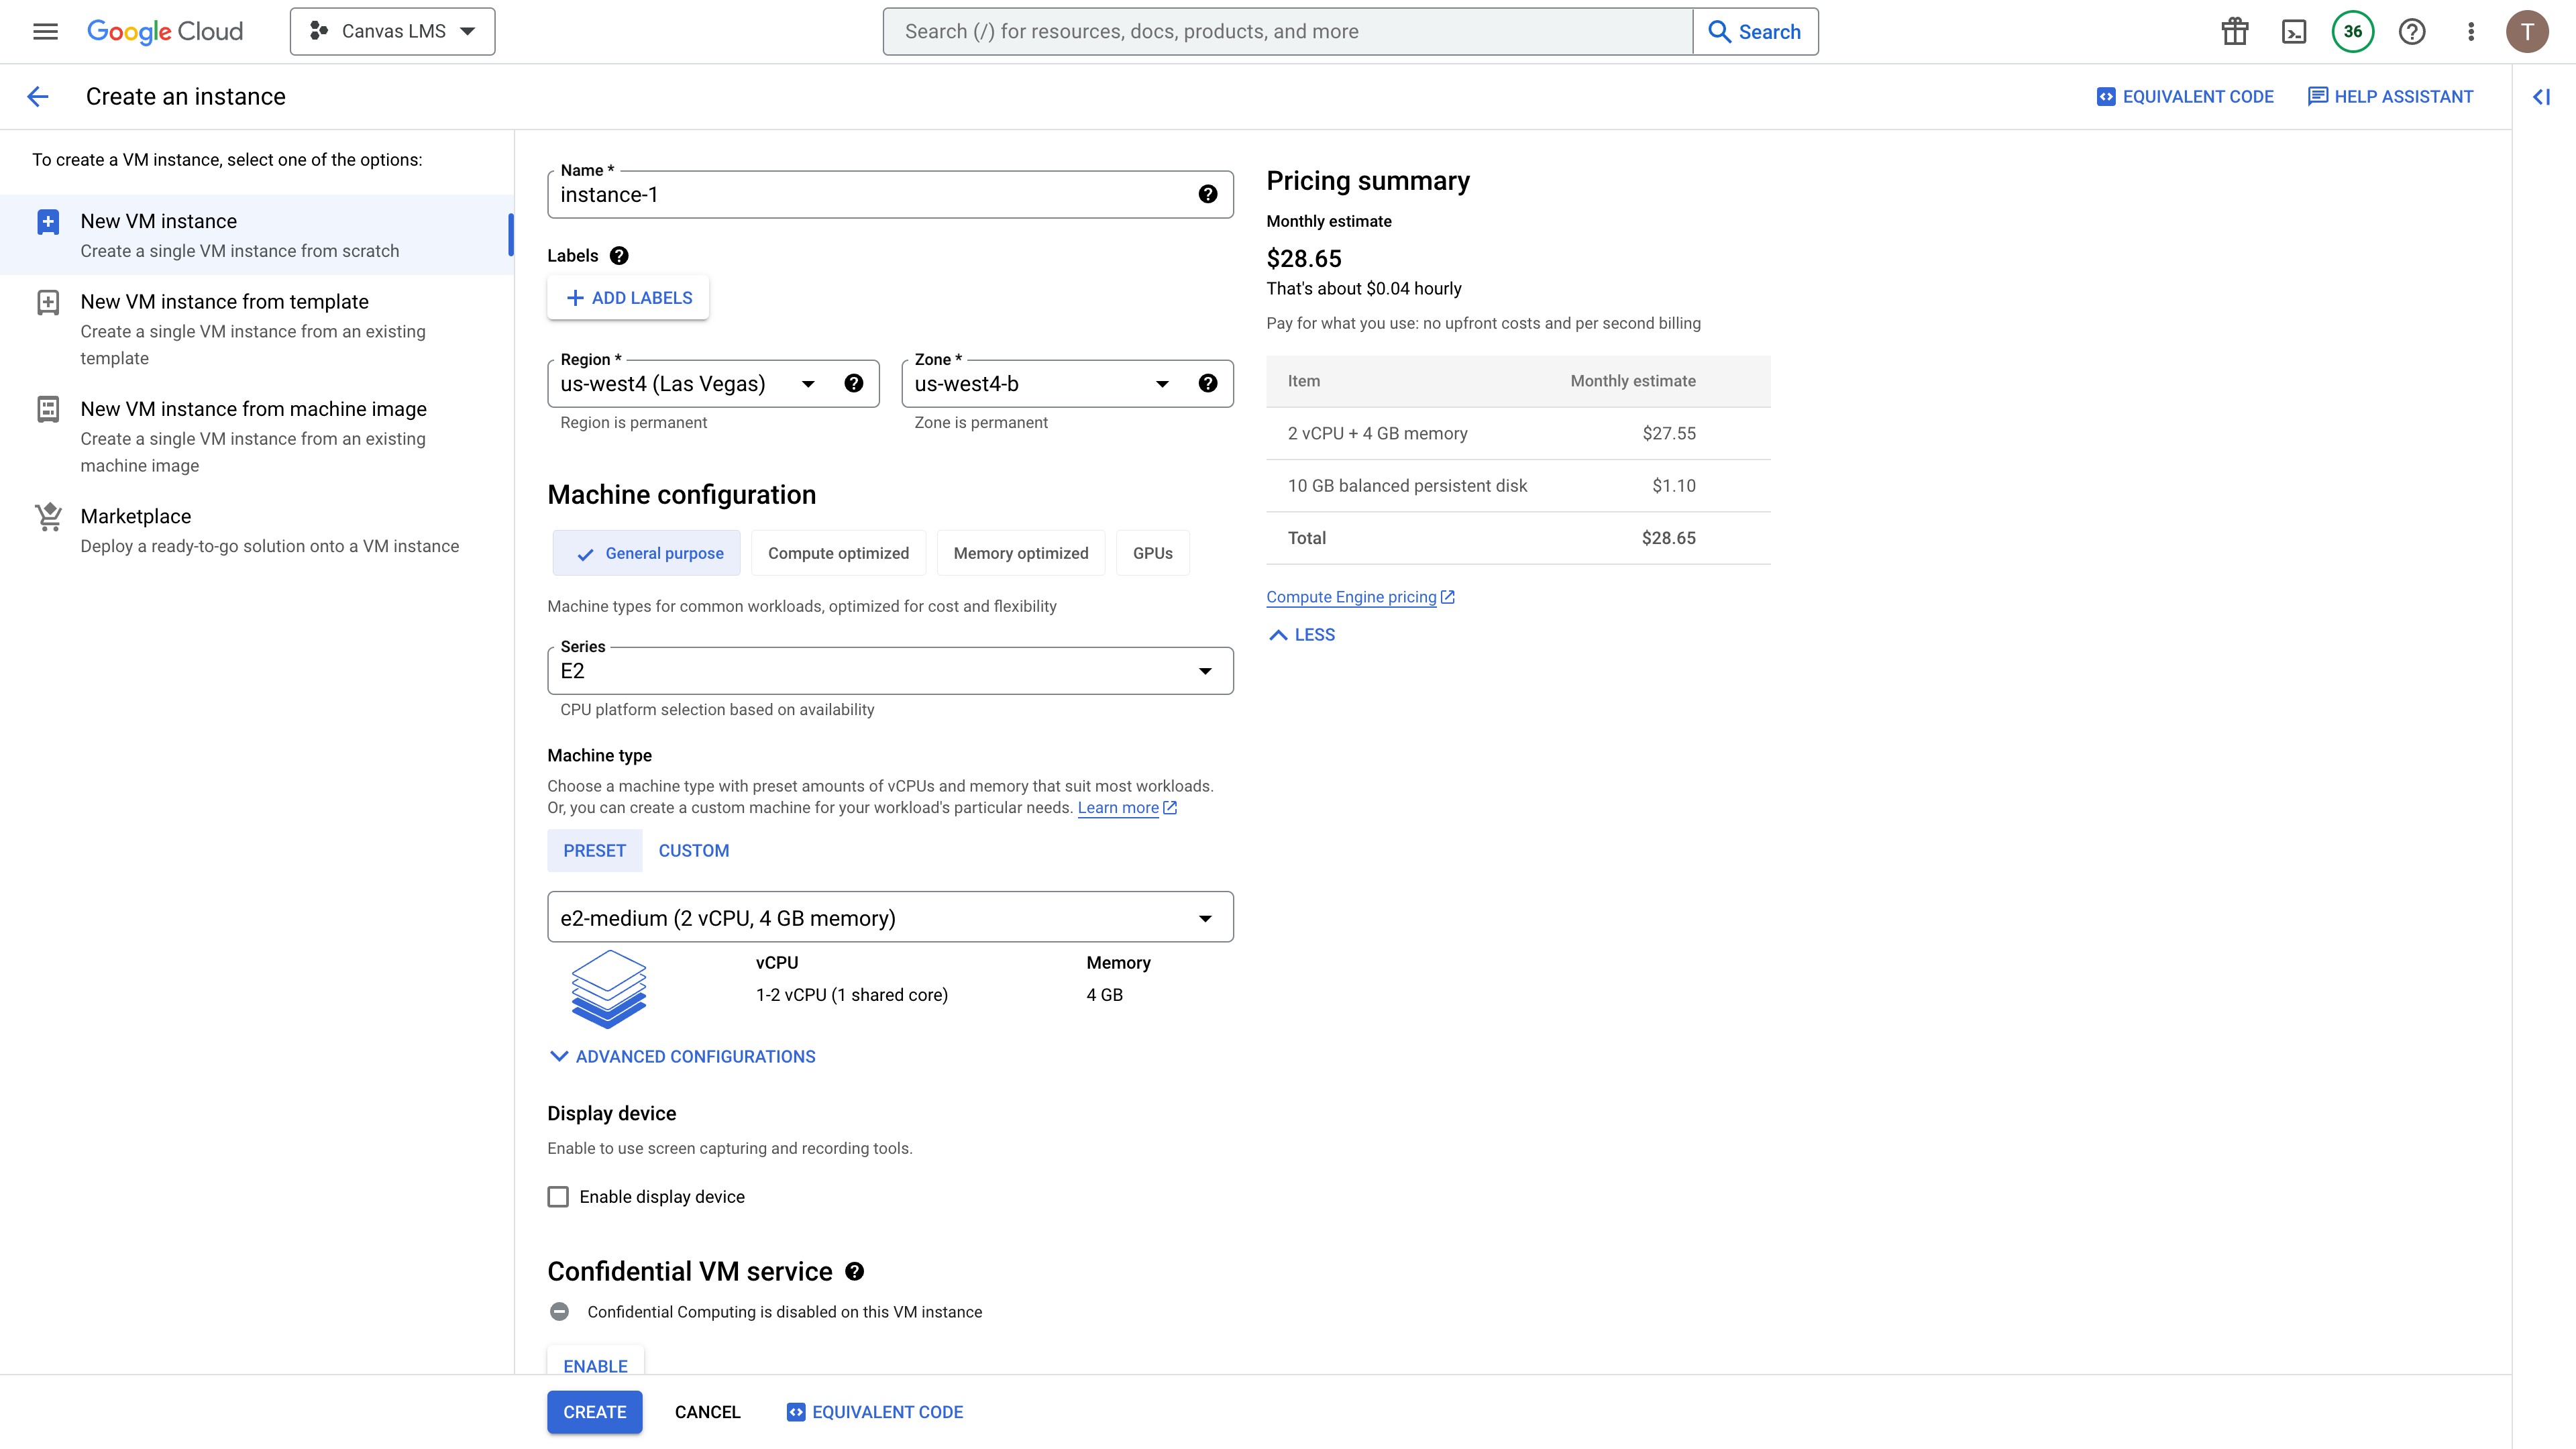
\includegraphics[width=300pt]{google-create-instance}
            \caption{Màn hình tạo máy ảo}
            \label{fig:google-create-instance}
        \end{figure}

        \item Cấu hình mạng: Đảm bảo rằng máy ảo của bạn được cấu hình để có địa chỉ IP công cộng và có quyền truy cập Internet. Điều này sẽ đảm bảo rằng máy ảo có thể truy cập vào các tài nguyên cần thiết và có thể phục vụ các yêu cầu từ người dùng.

        Trên bảng điều khiển Google Cloud, chúng ta có thể cấu hình các thiết lập mạng cho máy ảo bằng cách điều hướng đến mục "Network" hoặc "Mạng" trên bảng điều khiển.
        
        Ở đây, chúng ta có thể thực hiện các tác vụ như gán địa chỉ IP công cộng, tạo và quản lý các quy tắc tường lửa, cấu hình phân giải tên miền và nhiều hơn nữa.

        \begin{figure}[ht!]
            \centering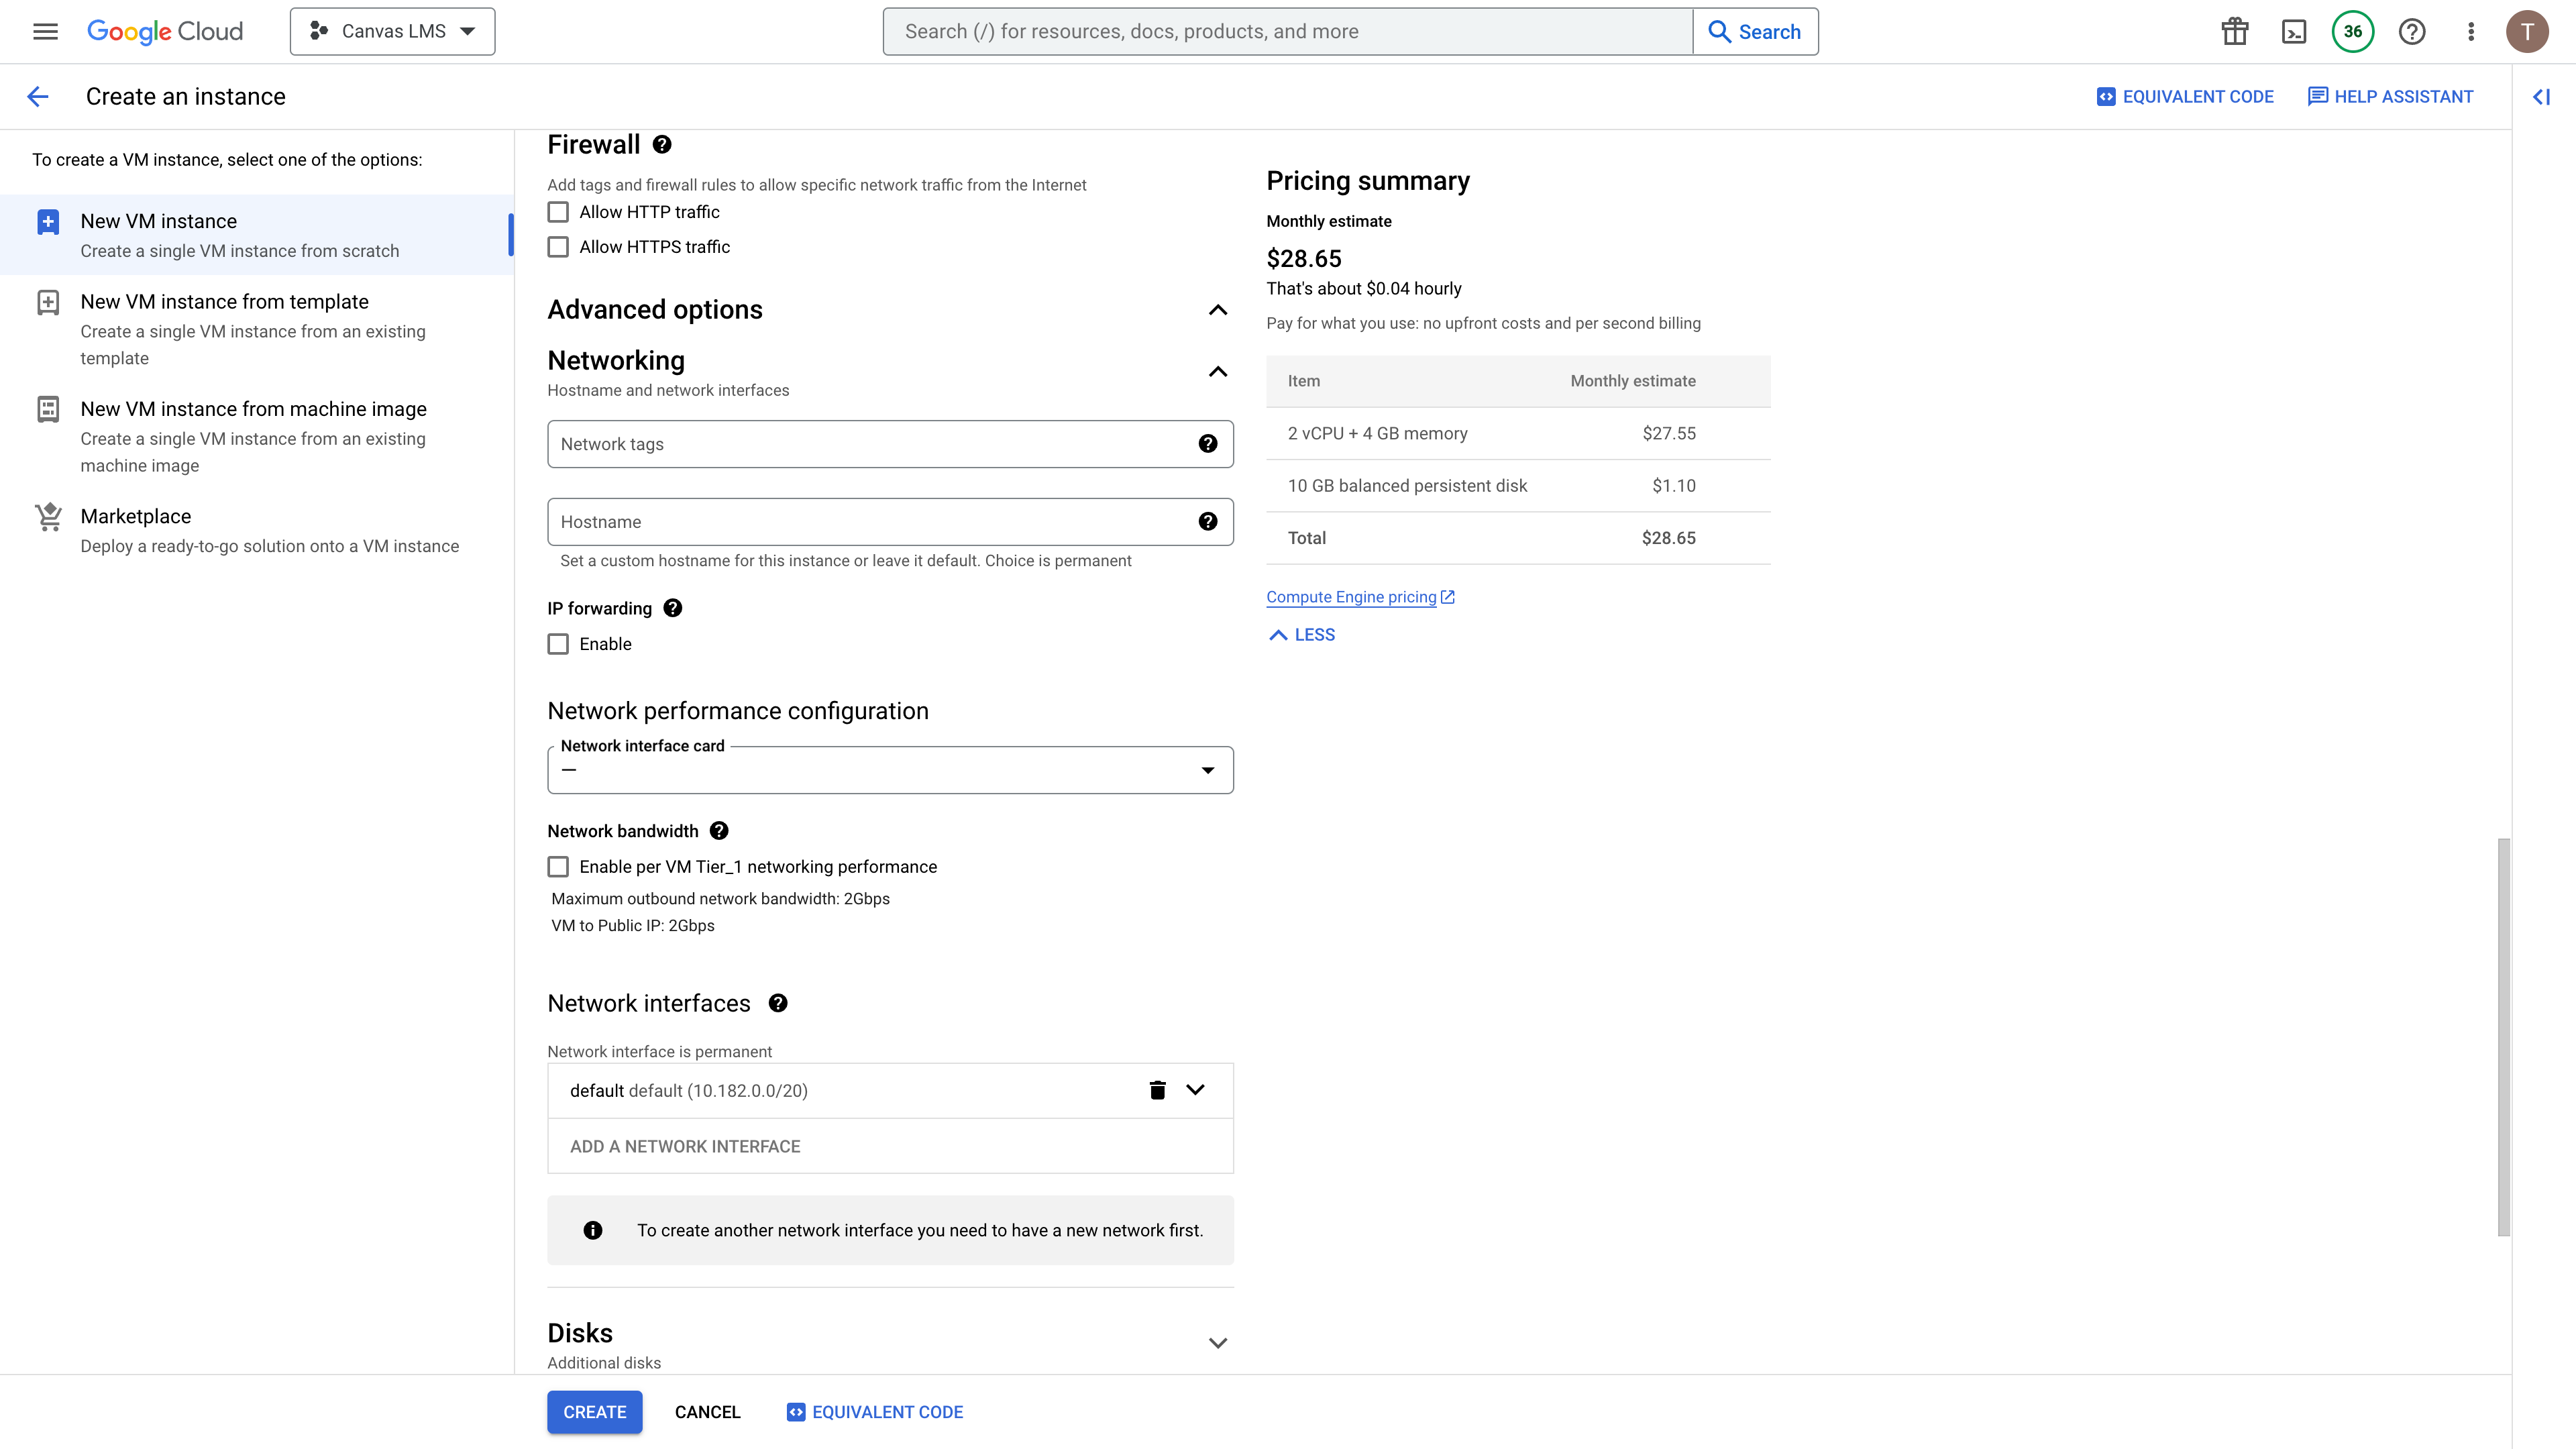
\includegraphics[width=300pt]{google-network}
            \caption{Cài đặt mạng cho máy ảo}
            \label{fig:google-network}
        \end{figure}

        \item Cài đặt và cấu hình Canvas LMS: Sau khi đã chuẩn bị môi trường, chúng ta có thể tiến hành cài đặt và cấu hình Canvas LMS trên máy ảo. Quá trình này bao gồm cài đặt Ruby, PostgreSQL, các gói phụ thuộc và mã nguồn Canvas LMS.

        Để cài đặt và cấu hình Canvas LMS, chúng ta sẽ sử dụng các lệnh và tệp cấu hình được cung cấp trong mã nguồn của Canvas LMS. Quá trình này yêu cầu kiến thức về quản lý máy chủ và cài đặt ứng dụng web.
        
        Sau khi cài đặt và cấu hình thành công, chúng ta sẽ có một môi trường Canvas LMS hoạt động trên máy ảo của chúng ta trên Google Cloud.
    \end{enumerate}
    \subsection{Cài đặt Canvas LMS}
        \begin{enumerate}
            \item Cài đặt Ruby: Canvas LMS yêu cầu phiên bản Ruby 2.7.3. Để cài đặt phiên bản này, chúng ta sẽ sử dụng RVM (Ruby Version Manager). RVM là một công cụ quản lý phiên bản Ruby cho phép chúng ta cài đặt nhiều phiên bản Ruby trên cùng một máy tính.

            Để cài đặt RVM, chúng ta sẽ sử dụng lệnh sau:
            \begin{lstlisting}[language=bash]
                $ curl -sSL https://rvm.io/mpapis.asc | gpg --import -
                $ curl -sSL https://get.rvm.io | bash -s stable
            \end{lstlisting}

            Sau khi cài đặt RVM, chúng ta sẽ cài đặt phiên bản Ruby 2.7.3 bằng lệnh sau:
            \begin{lstlisting}[language=bash]
                $ rvm install 2.7.3
            \end{lstlisting}

            \item Cài đặt PostgreSQL: Canvas LMS yêu cầu phiên bản PostgreSQL 9.5. Để cài đặt phiên bản này, chúng ta sẽ sử dụng các lệnh sau:
            \begin{lstlisting}[language=bash]
                $ sudo apt-get update
                $ sudo apt-get install postgresql postgresql-contrib
            \end{lstlisting}

            Sau khi cài đặt PostgreSQL, chúng ta sẽ tạo một người dùng và một cơ sở dữ liệu cho Canvas LMS. Để làm điều này, chúng ta sẽ sử dụng các lệnh sau:
            \begin{lstlisting}[language=bash]
                $ sudo -u postgres createuser canvas --no-createdb --no-superuser --no-createrole --pwprompt
                $ sudo -u postgres createdb canvas_production --owner=canvas
            \end{lstlisting}

            \item Cài đặt các gói phụ thuộc: Canvas LMS yêu cầu một số gói phụ thuộc để có thể hoạt động. Để cài đặt các gói phụ thuộc này, chúng ta sẽ sử dụng các lệnh sau:
            \begin{lstlisting}[language=bash]
                $ sudo apt-get install git-core curl zlib1g-dev build-essential libssl-dev libreadline-dev libyaml-dev libsqlite3-dev sqlite3 libxml2-dev libxslt1-dev libcurl4-openssl-dev software-properties-common libffi-dev
            \end{lstlisting}

            \item Cài đặt mã nguồn Canvas LMS: Sau khi đã cài đặt các gói phụ thuộc, chúng ta sẽ tiến hành cài đặt mã nguồn Canvas LMS. Để làm điều này, chúng ta sẽ sử dụng các lệnh sau:
            \begin{lstlisting}[language=bash]
                $ cd ~
                $ git clone https://github.com/instructure/canvas-lms.git canvas
                $ cd canvas
                $ git checkout prod
                $ sudo mkdir -p /var/canvas
                $ sudo chown -R $USER /var/canvas
                $ cp -av . /var/canvas
            \end{lstlisting}

            \item Càu đặt yarn sau khi đã cài đặt mã nguồn Canvas LMS: Canvas LMS yêu cầu yarn để có thể hoạt động. Để cài đặt yarn, chúng ta sẽ sử dụng các lệnh sau:
            \begin{lstlisting}[language=bash]
                $ curl -sS https://dl.yarnpkg.com/debian/pubkey.gpg | sudo apt-key add -
                $ echo "deb https://dl.yarnpkg.com/debian/ stable main" | sudo tee /etc/apt/sources.list.d/yarn.list
                $ sudo apt-get update
                $ sudo apt-get install yarn
            \end{lstlisting}

            \item Cài đặt các gói phụ thuộc của Canvas LMS: Sau khi đã cài đặt yarn, chúng ta sẽ tiến hành cài đặt các gói phụ thuộc của Canvas LMS. Để làm điều này, chúng ta sẽ sử dụng các lệnh sau:
            \begin{lstlisting}[language=bash]
                $ cd /var/canvas
                $ bundle config set path 'vendor/bundle'
                $ yarn install
            \end{lstlisting}



            \item Cấu hình Canvas LMS: Sau khi đã cài đặt yarn, chúng ta sẽ tiến hành cấu hình Canvas LMS. Để làm điều này, chúng ta sẽ sử dụng các lệnh sau:
            \begin{lstlisting}[language=bash]
                $ cp config/database.yml.example config/database.yml
                $ nano config/database.yml
                $ bundle exec rake canvas:compile_assets
            \end{lstlisting}

            \item Cấu hình Apache: Sau khi đã cấu hình Canvas LMS, chúng ta sẽ tiến hành cấu hình Apache. Để làm điều này, chúng ta sẽ sử dụng các lệnh sau:

            Đầu tiên, chúng ta sẽ cài đặt Apache bằng lệnh sau:
            \begin{lstlisting}[language=bash]
                $ sudo apt-get install apache2
                $ sudo apt-get install -y libapache2-mod-passenger
            \end{lstlisting}

            Sau đó, chúng ta sẽ cấu hình Apache bằng lệnh sau:
            \begin{lstlisting}[language=bash]
                $ sudo nano /etc/apache2/sites-available/canvas.conf
            \end{lstlisting}

            Trong file cấu hình này, chúng ta sẽ thêm các dòng sau:
            \begin{lstlisting}[language=bash]
                <VirtualHost *:80>
                    ServerName 35.247.158.82
                    ServerAlias canvasfiles.example.com
                    ServerAdmin brad@sandbox84e1f41fa65f4f75941861cde77b288a.mailgun.org
                    DocumentRoot /var/canvas/public
                    RewriteEngine On
                    RewriteCond %{HTTP:X-Forwarded-Proto} !=https
                    RewriteCond %{REQUEST_URI} !^/health_check
                    RewriteRule (.*) https://%{HTTP_HOST}%{REQUEST_URI} [L]
                    ErrorLog /var/log/apache2/canvas_errors.log
                    LogLevel warn
                    CustomLog /var/log/apache2/canvas_access.log combined
                    SetEnv RAILS_ENV production
                    <Directory /var/canvas/public>
                        Options All
                        AllowOverride All
                        Require all granted
                    </Directory>
                </VirtualHost>
                    # If you are only serving HTTP behind a HTTPS-terminating load balancer, skip the next VirtualHost
                <VirtualHost *:443>
                    ServerName 35.247.158.82
                    ServerAlias canvasfiles.example.com
                    ServerAdmin brad@sandbox84e1f41fa65f4f75941861cde77b288a.mailgun.org
                    DocumentRoot /var/canvas/public
                    ErrorLog /var/log/apache2/canvas_errors.log
                    LogLevel warn
                    CustomLog /var/log/apache2/canvas_ssl_access.log combined
                    SSLEngine on
                    BrowserMatch "MSIE [17-9]" ssl-unclean-shutdown
                    # the following ssl certificate files are generated for you from the ssl-cert package.
                    SSLCertificateFile /etc/ssl/certs/ssl-cert-snakeoil.pem
                    SSLCertificateKeyFile /etc/ssl/private/ssl-cert-snakeoil.key
                    SetEnv RAILS_ENV production
                    <Directory /var/canvas/public>
                        Options All
                        AllowOverride All
                        Require all granted
                    </Directory>
                </VirtualHost>
            \end{lstlisting}

            Sau đó, chúng ta sẽ cấu hình Apache bằng lệnh sau:
            \begin{lstlisting}[language=bash]
                $ sudo a2enmod ssl
                $ sudo a2enmod headers
                $ sudo a2ensite canvas
                $ sudo a2enmod rewrite
                $ sudo a2dissite 000-default
                $ sudo service apache2 restart
            \end{lstlisting}

            \item Cấu hình Canvas LMS: Sau khi đã cấu hình Apache, chúng ta sẽ tiến hành cấu hình Canvas LMS. Để làm điều này, chúng ta sẽ sử dụng các lệnh sau:
            
            Đầu tiên, chúng ta sẽ cấu hình Canvas LMS bằng lệnh sau:
            \begin{lstlisting}[language=bash]
                $ cp config/outgoing_mail.yml.example config/outgoing_mail.yml
                $ nano config/outgoing_mail.yml
            \end{lstlisting}

            Trong file cấu hình này, chúng ta sẽ thêm các dòng sau:
            \begin{lstlisting}[language=bash]
                production:
                    address: "smtp.mailgun.org"
                    port: "587"
                    user_name: "postmaster@sandbox84e1f41fa65f4f75941861cde77b288a.mailgun.org"
                    password: "thuongkhung120"
                    authentication: "login" # plain, login, or cram_md5
                    domain: "sandbox84e1f41fa65f4f75941861cde77b288a.mailgun.org"
                    outgoing_address: "thuongkhungvu@gmail.com"
                    default_name: "Thuy Loi University"
            \end{lstlisting}

            Sau đó, chúng ta sẽ cấu hình Canvas LMS bằng lệnh sau:
            \begin{lstlisting}[language=bash]
                $ cp config/domain.yml.example config/domain.yml
                $ nano config/domain.yml
            \end{lstlisting}

            Trong file cấu hình này, chúng ta sẽ thêm các dòng sau:
            \begin{lstlisting}[language=bash]
                production:
                    domain: "35.247.158.82"
                    ssl: true
            \end{lstlisting}

            Sau đó, chúng ta sẽ cấu hình Canvas LMS bằng lệnh sau:
            \begin{lstlisting}[language=bash]
                $ cp config/security.yml.example config/security.yml
                $ nano config/security.yml
            \end{lstlisting}

            Trong file cấu hình này, chúng ta sẽ thêm các dòng sau:
            \begin{lstlisting}[language=bash]
                production: &default
                    encryption_key: jsn2hsydandsu299374msdmcbusnk213nfdu2
            \end{lstlisting}

            Sau đó, chúng ta sẽ cấu hình Canvas LMS bằng lệnh sau:
            \begin{lstlisting}[language=bash]
                $ cp config/cache_store.yml.example config/cache_store.yml
                $ nano config/cache_store.yml
            \end{lstlisting}

            Trong file cấu hình này, chúng ta sẽ thêm các dòng sau:
            \begin{lstlisting}[language=bash]
                production:
                    cache_store: redis_cache_store
            \end{lstlisting}

            Sau đó, chúng ta sẽ cấu hình Canvas LMS bằng lệnh sau:
            \begin{lstlisting}[language=bash]
                $ cp config/redis.yml.example config/redis.yml
                $ nano config/redis.yml
            \end{lstlisting}

            Trong file cấu hình này, chúng ta sẽ thêm các dòng sau:
            \begin{lstlisting}[language=bash]
                production:
                    servers:
                    - redis://localhost
            \end{lstlisting}

            Sau khi đã cài đặt xong các gói cần thiết, chúng ta sẽ tiến hành cài đặt Canvas LMS bằng lệnh sau:
            \begin{lstlisting}[language=bash]
                $ bundle install --deployment --without development test postgres
                $ bundle exec rake db:create
                $ bundle exec rake db:initial_setup
                $ bundle exec rake canvas:compile_assets
            \end{lstlisting}

            Sau khi đã cài đặt xong Canvas LMS, chúng ta sẽ tiến hành cấu hình Canvas LMS bằng lệnh sau:
            \begin{lstlisting}[language=bash]
                $ cp config/production.example.yml config/production.yml
                $ nano config/production.yml
            \end{lstlisting}

            Trong file cấu hình này, chúng ta sẽ thêm các dòng sau:
            \begin{lstlisting}[language=bash]
                production:
                    domain: "35.247.158.82"
                    ssl: true
            \end{lstlisting}

            Sau khi đã cấu hình xong Canvas LMS, chúng ta sẽ tiến hành cài đặt Canvas LMS bằng lệnh sau:
            \begin{lstlisting}[language=bash]
                $ bundle exec rake canvas:compile_assets
            \end{lstlisting}

        Sau khi hoàn thành cài đặt, chúng ta sẽ tiến hành khởi động lại Canvas LMS bằng lệnh sau:
            \begin{lstlisting}[language=bash]
                $ sudo /etc/init.d/apache2 restart
            \end{lstlisting}

            Sau khi khởi động lại Canvas LMS, chúng ta sẽ truy cập vào địa chỉ \url{http://35.247.158.82} để kiểm tra kết quả.
        \end{enumerate}

    \subsection{Xây dựng phần giao diện cho hệ thống}
    \label{subsec:xay-dung-giao-dien}
    \subsubsection{Xây dựng giao diện chung}
    \label{subsubsec:xay-dung-giao-dien-chung}
        Phần landing page của hệ thống được thể hiện ở hình:
        \begin{figure}[ht!]
            \centering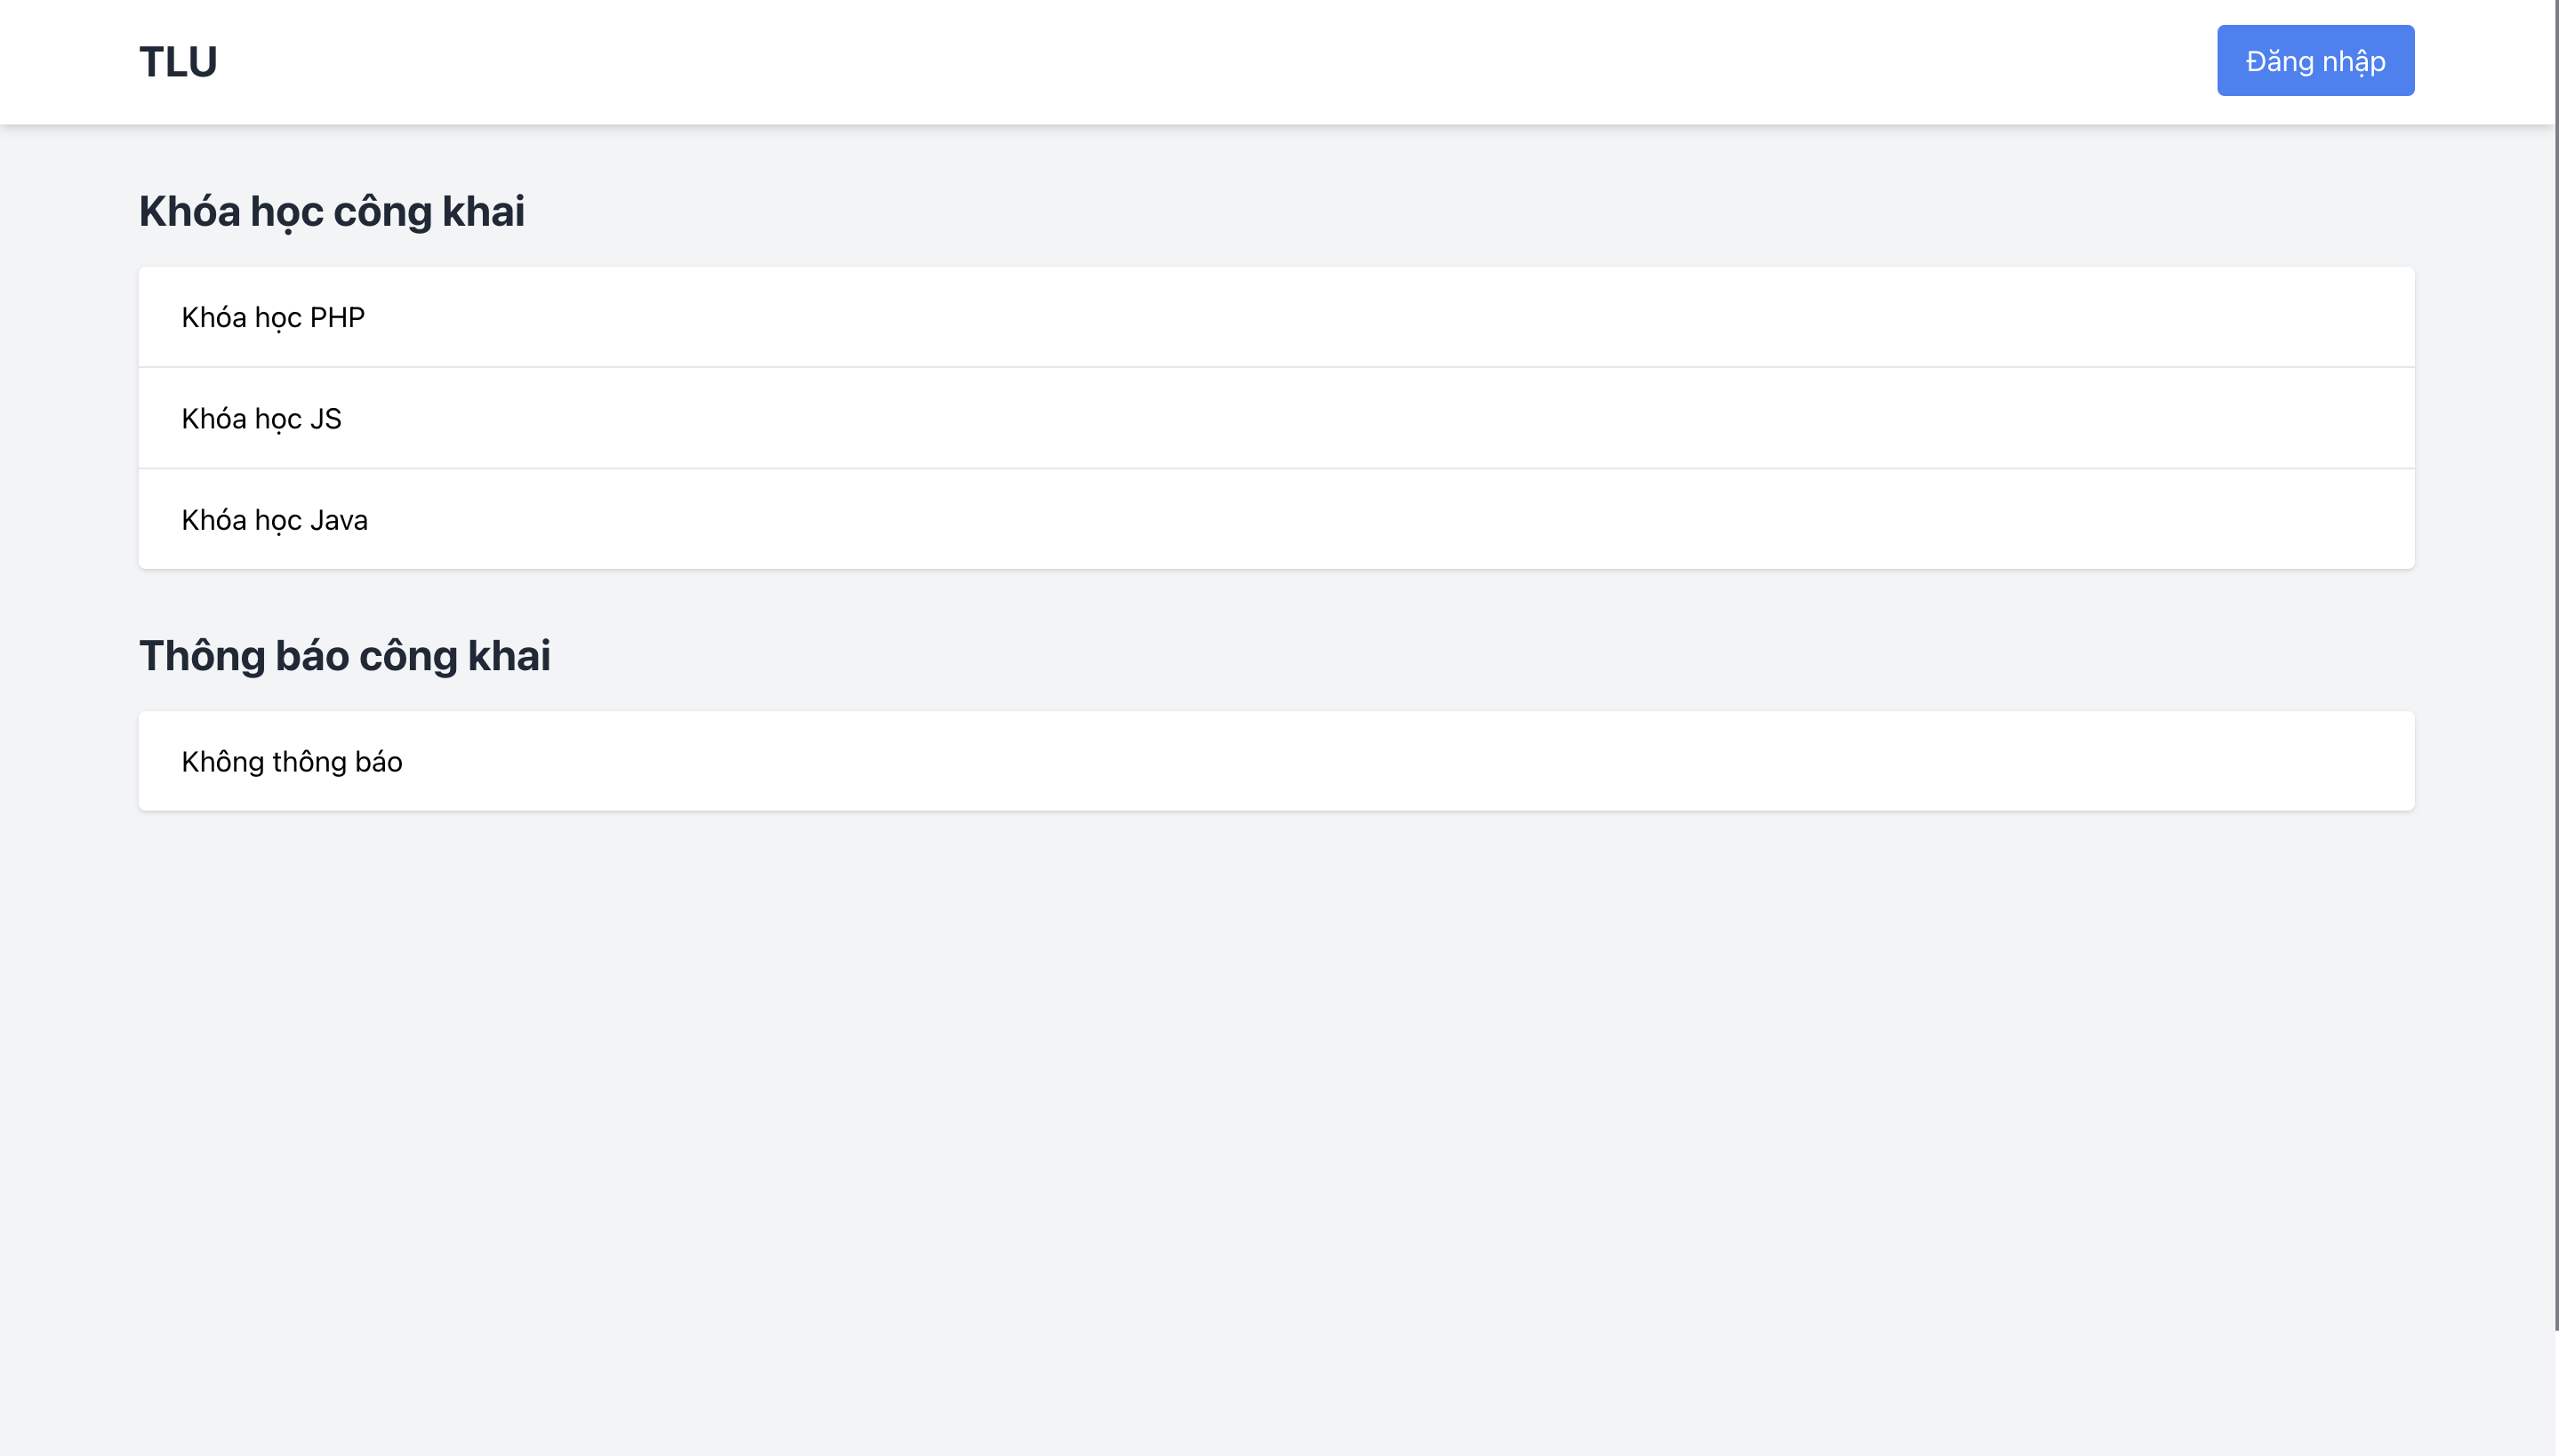
\includegraphics[width=300pt]{landing-page}
            \caption{Màn hình landing page của hệ thống}
            \label{fig:landing-page}
        \end{figure}

    \subsubsection{Xây dựng giao diện cho phần quản trị viên}
    \label{subsubsec:xay-dung-giao-dien-admin}
    
        Phần đăng nhập của phần quản trị viên được thể hiện ở hình:
        \begin{figure}[ht!]
            \centering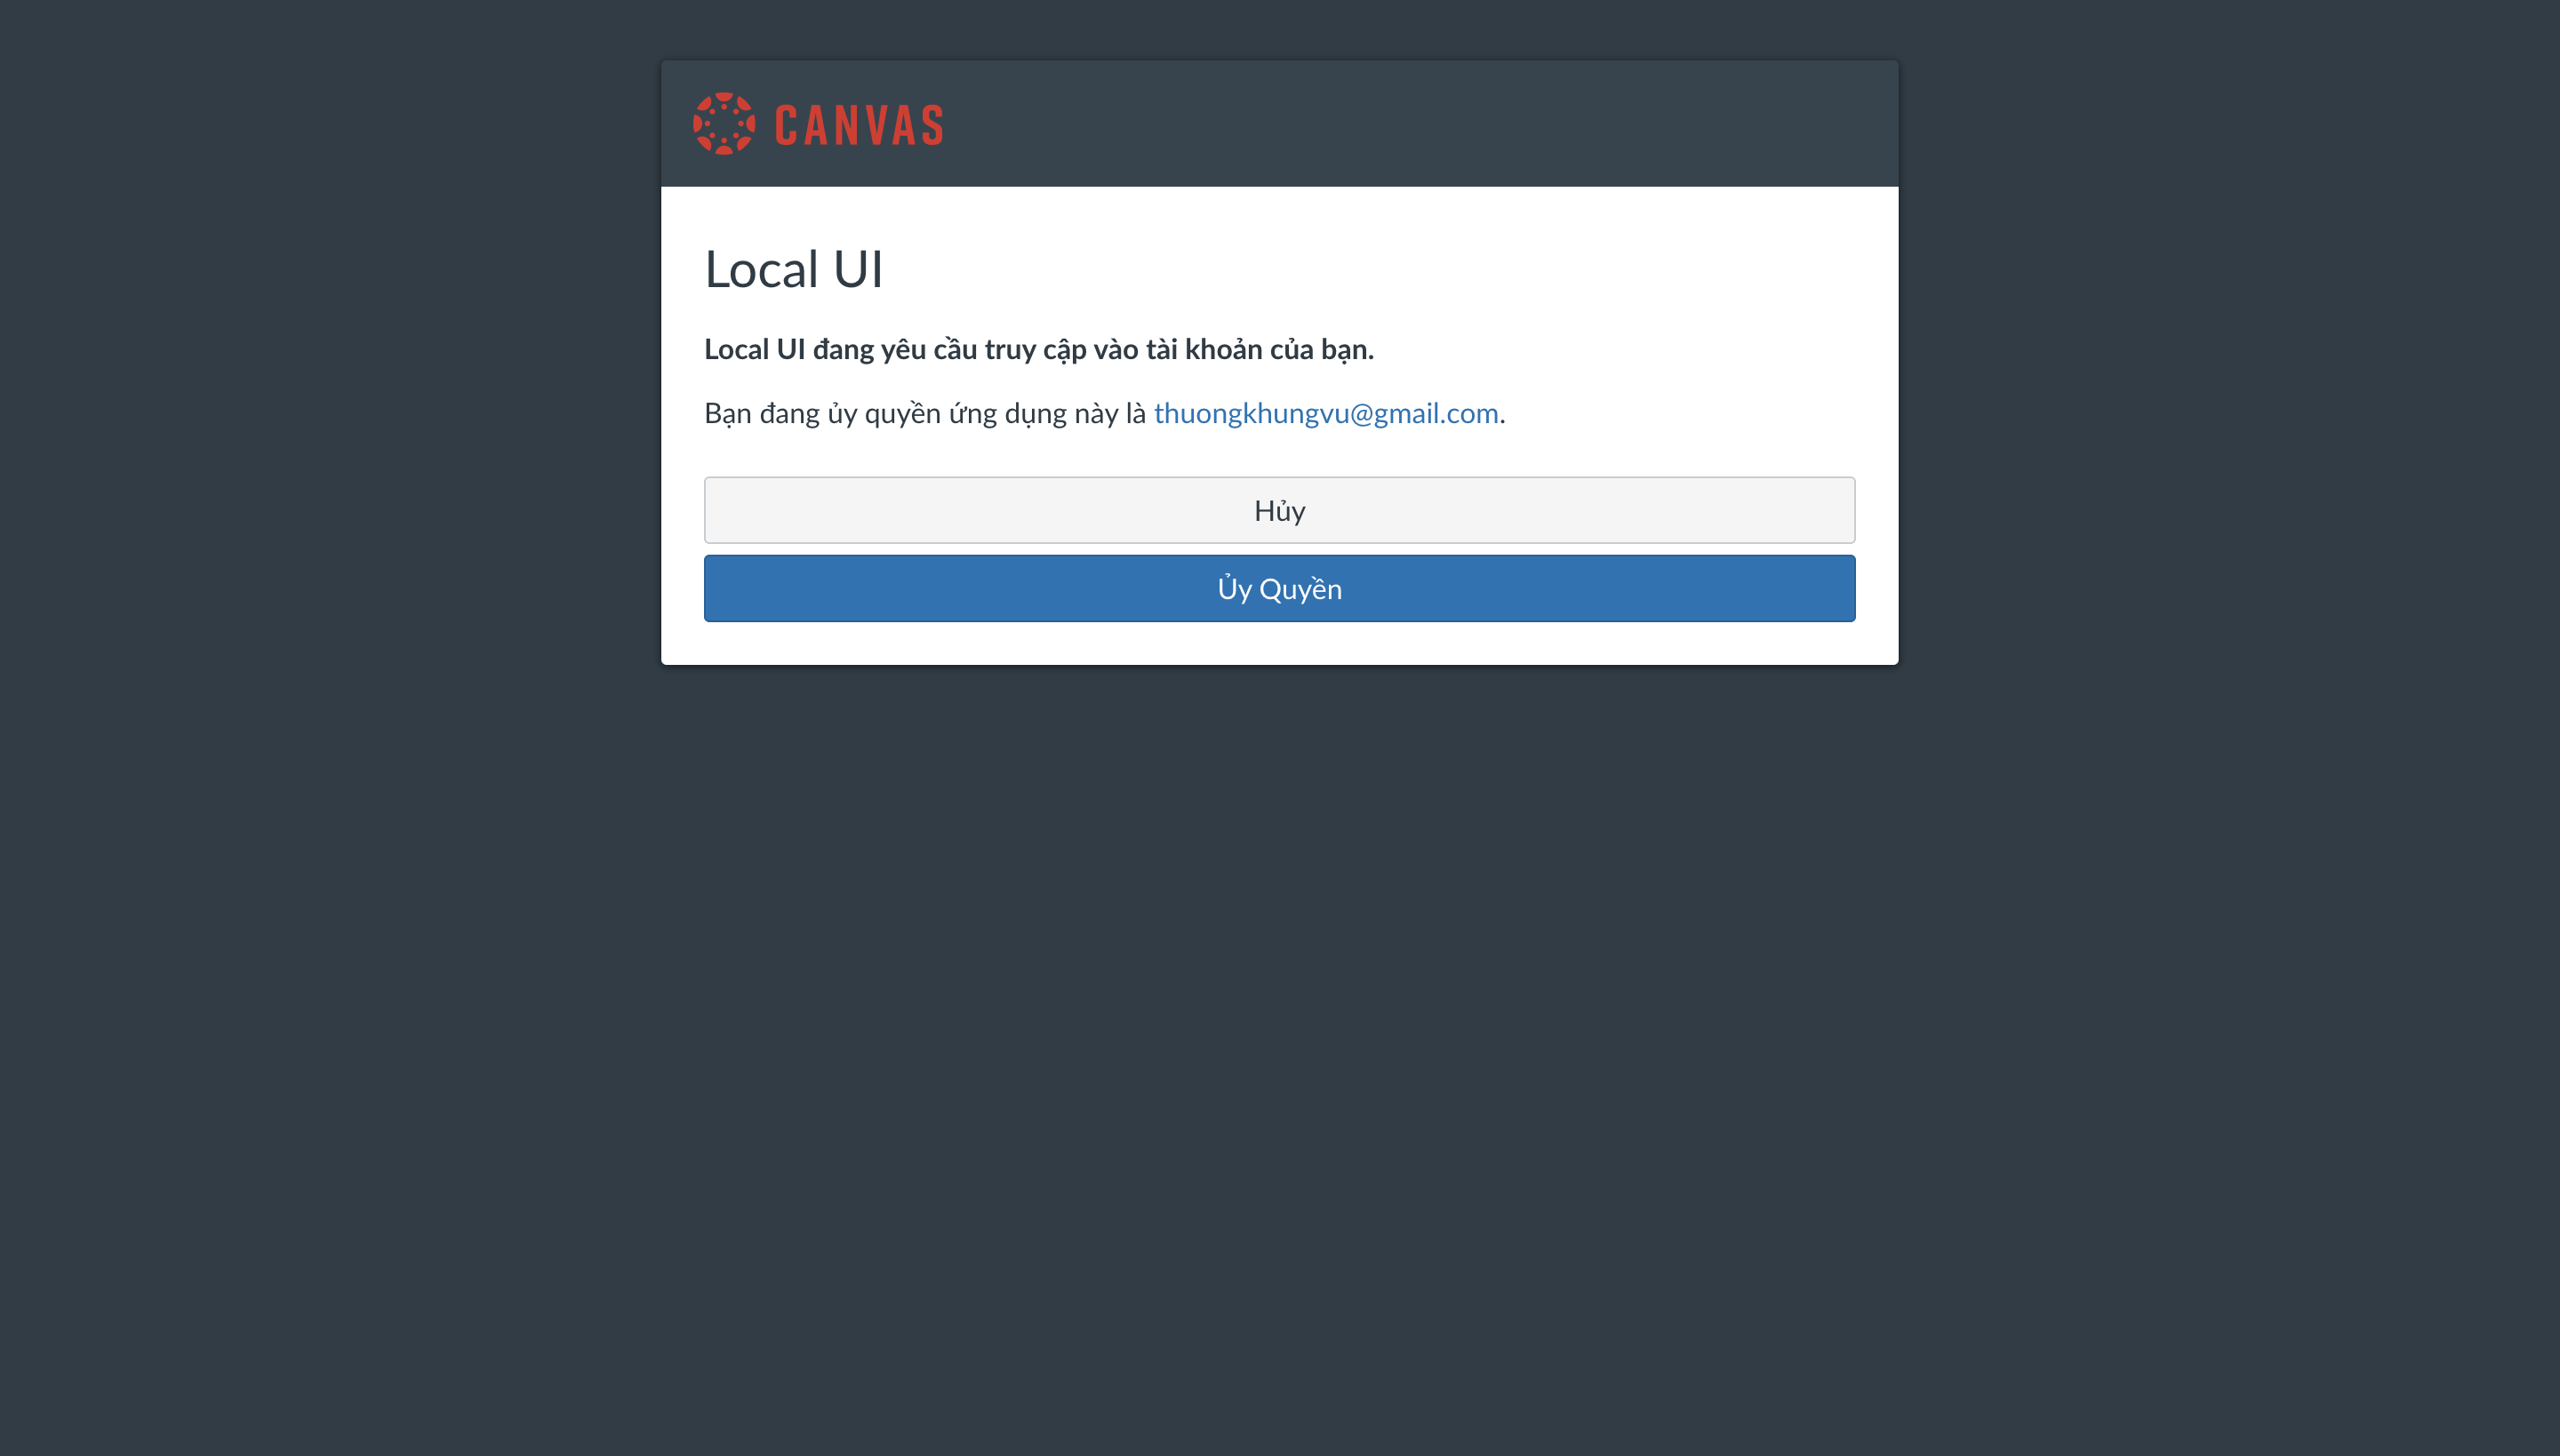
\includegraphics[width=300pt]{dang-nhap-admin}
            \caption{Màn hình đăng nhập của phần quản trị viên}
            \label{fig:dang-nhap-admin}
        \end{figure}

        Phần trang chủ của phần quản trị viên được thể hiện ở hình:
        \begin{figure}[ht!]
            \centering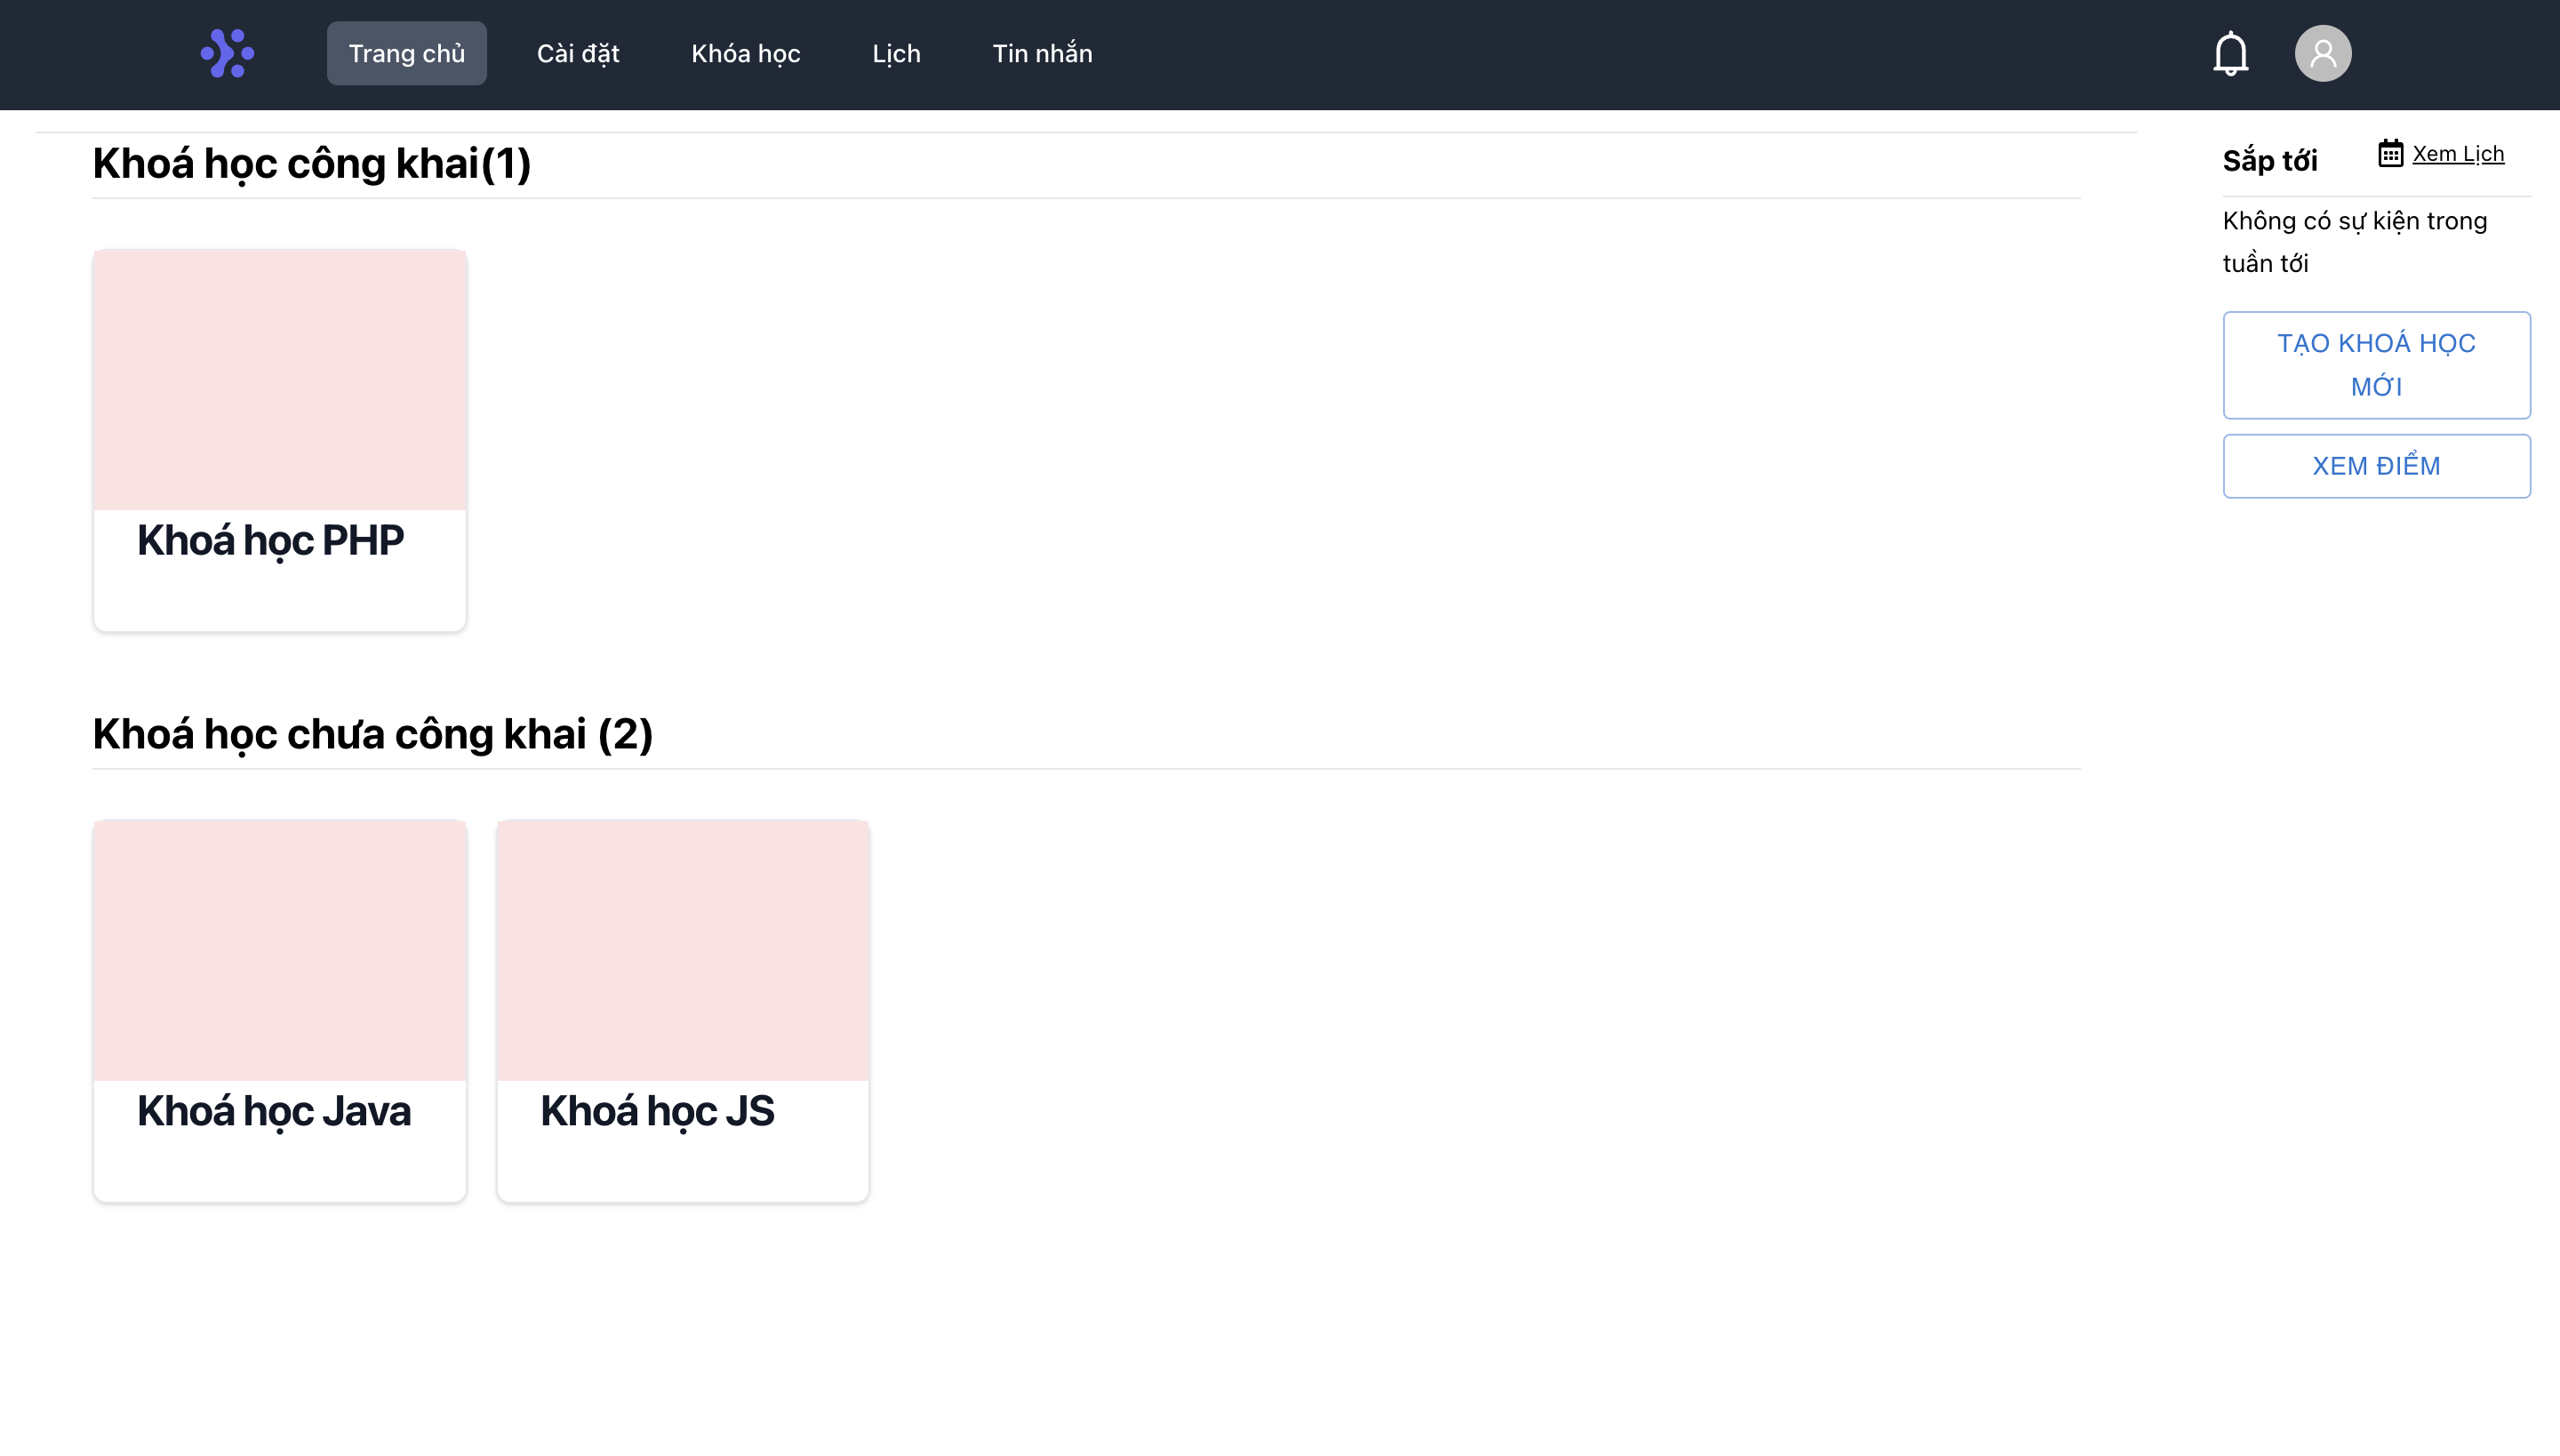
\includegraphics[width=300pt]{trang-chu-admin}
            \caption{Màn hình trang chủ của phần quản trị viên}
            \label{fig:trang-chu-admin}
        \end{figure}

        Phần danh sách khoá học của phần quản trị viên được thể hiện ở hình:
        \begin{figure}[ht!]
            \centering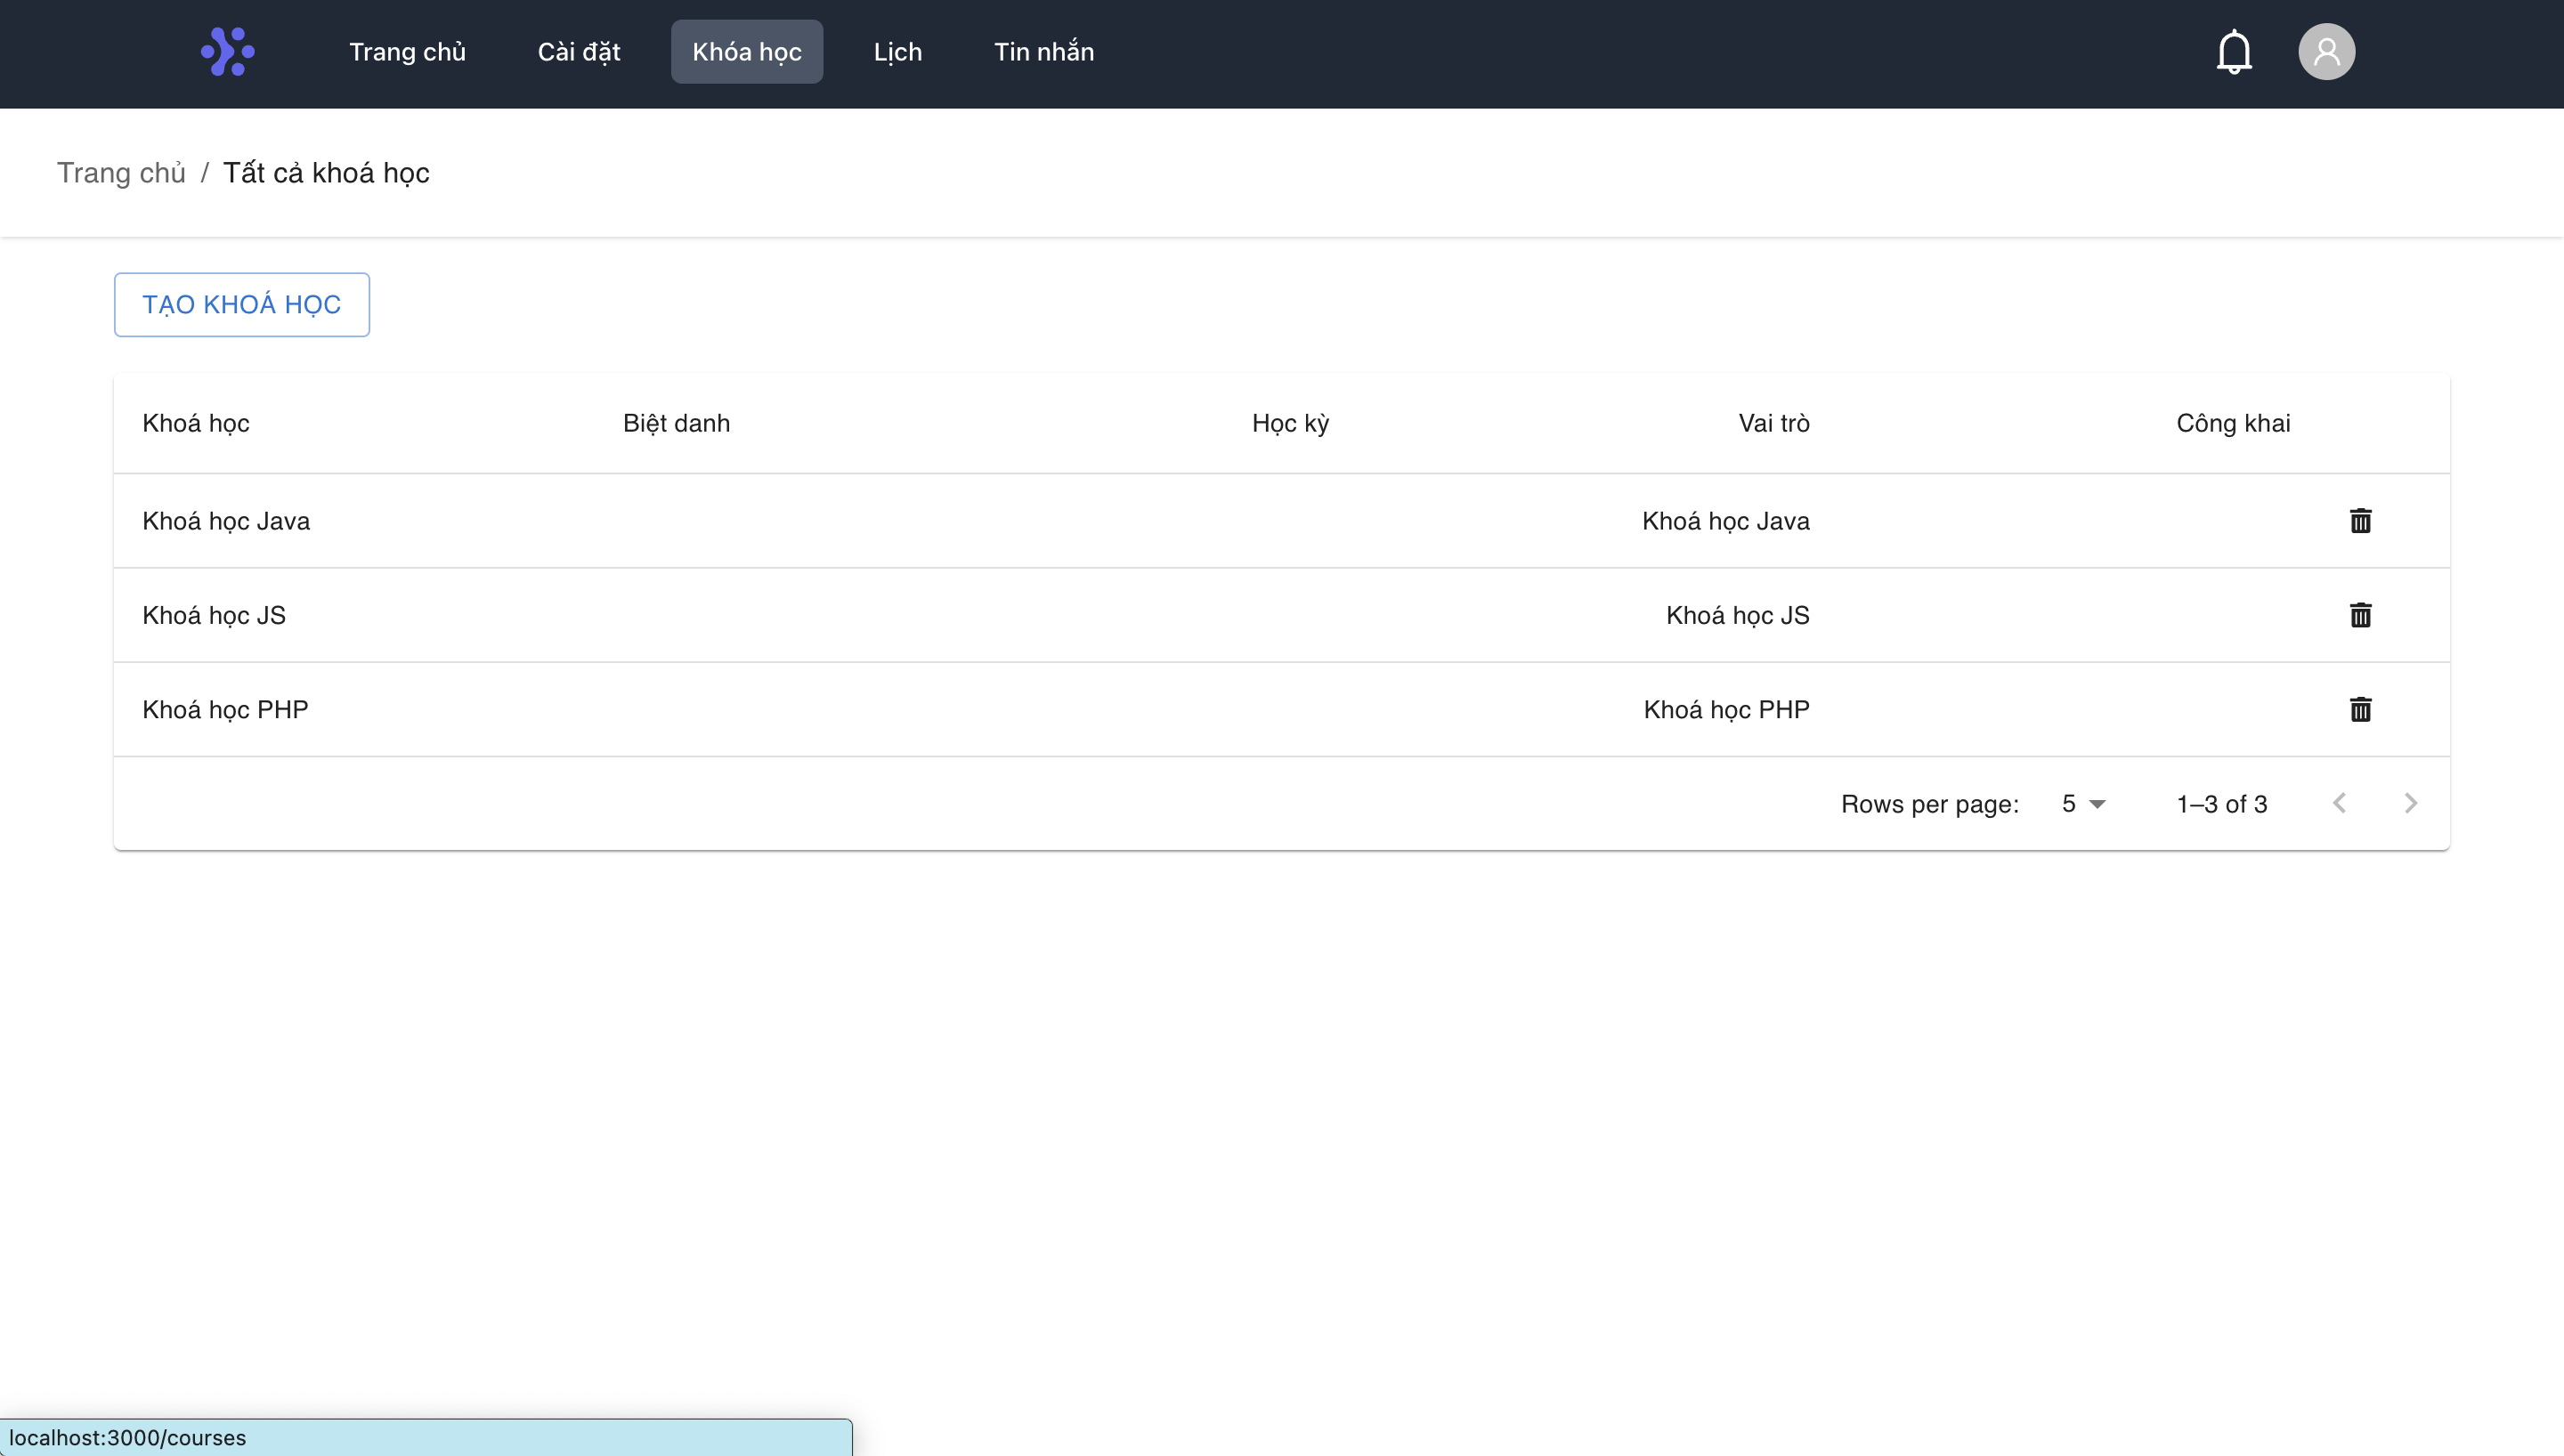
\includegraphics[width=300pt]{danh-sach-khoa-hoc}
            \caption{Màn hình danh sách khoá học của phần quản trị viên}
            \label{fig:danh-sach-khoa-hoc}
        \end{figure}

        Phần tạo khoá học của phần quản trị viên được thể hiện ở hình:
        \begin{figure}[ht!]
            \centering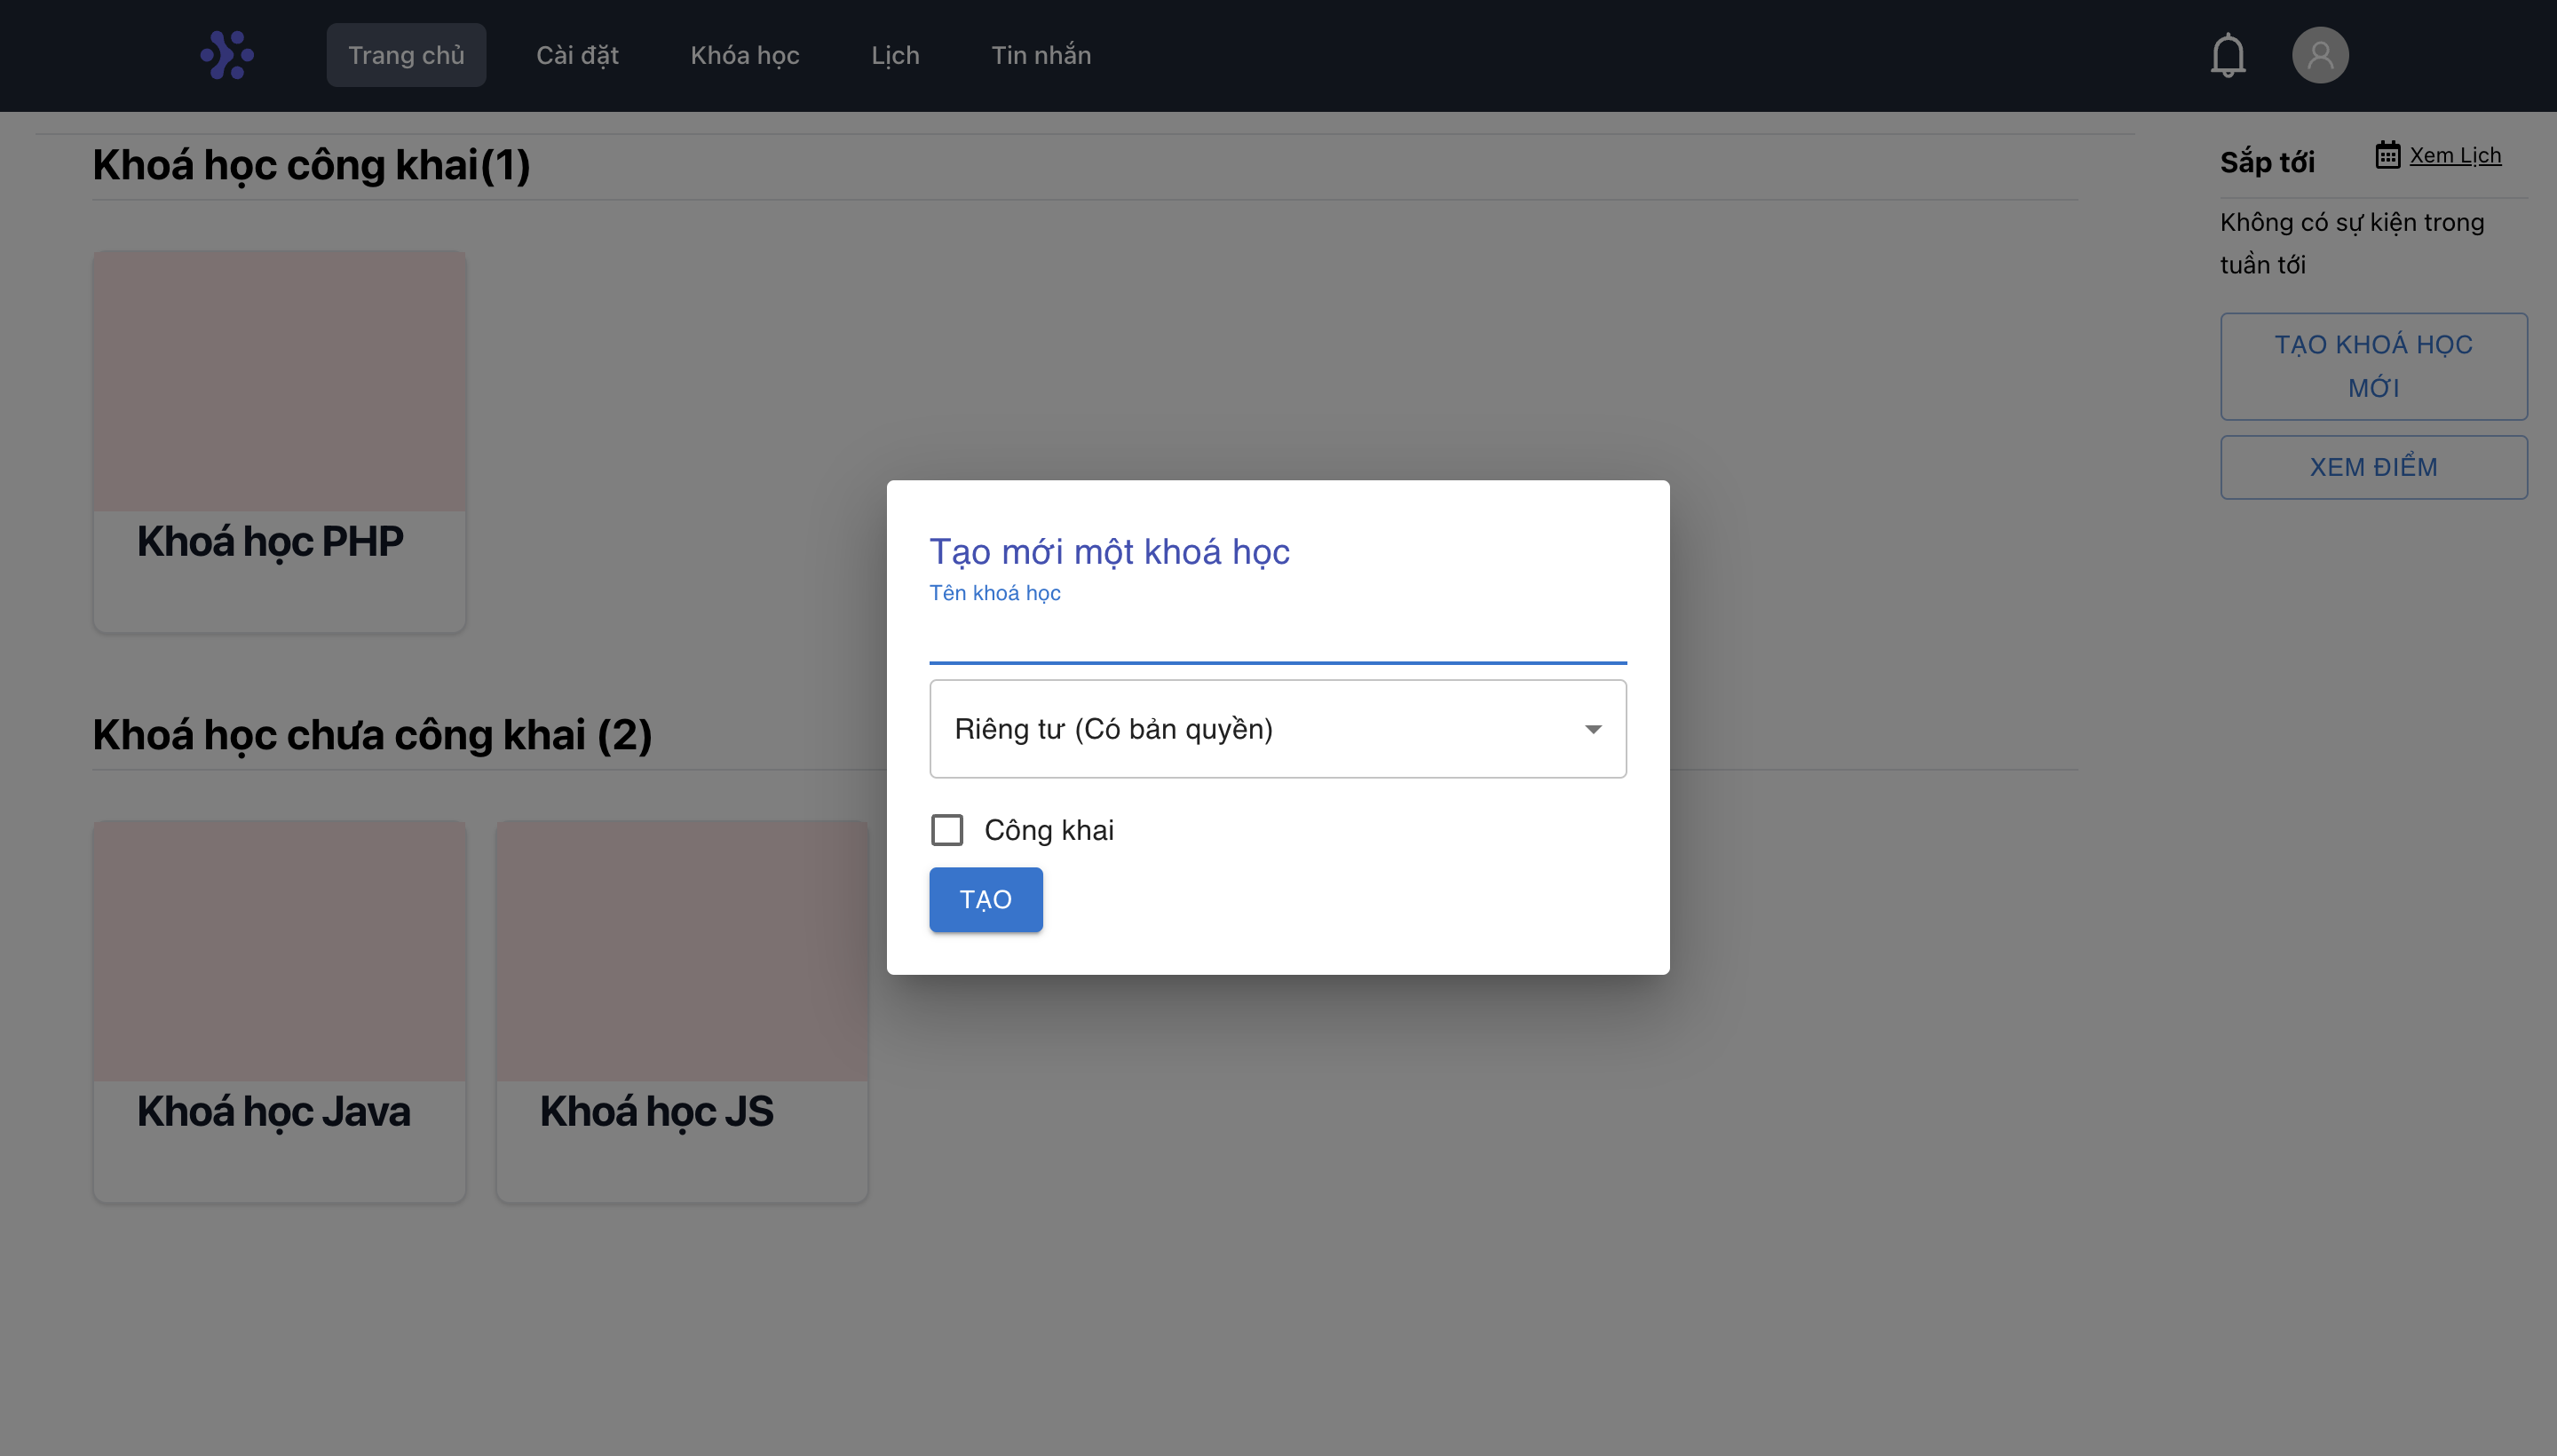
\includegraphics[width=300pt]{tao-khoa-hoc}
            \caption{Màn hình tạo khoá học của phần quản trị viên}
            \label{fig:tao-khoa-hoc}
        \end{figure}


        Phần danh sách bài tập và nhóm của phần quản trị viên được thể hiện ở hình:
        \begin{figure}[ht!]
            \centering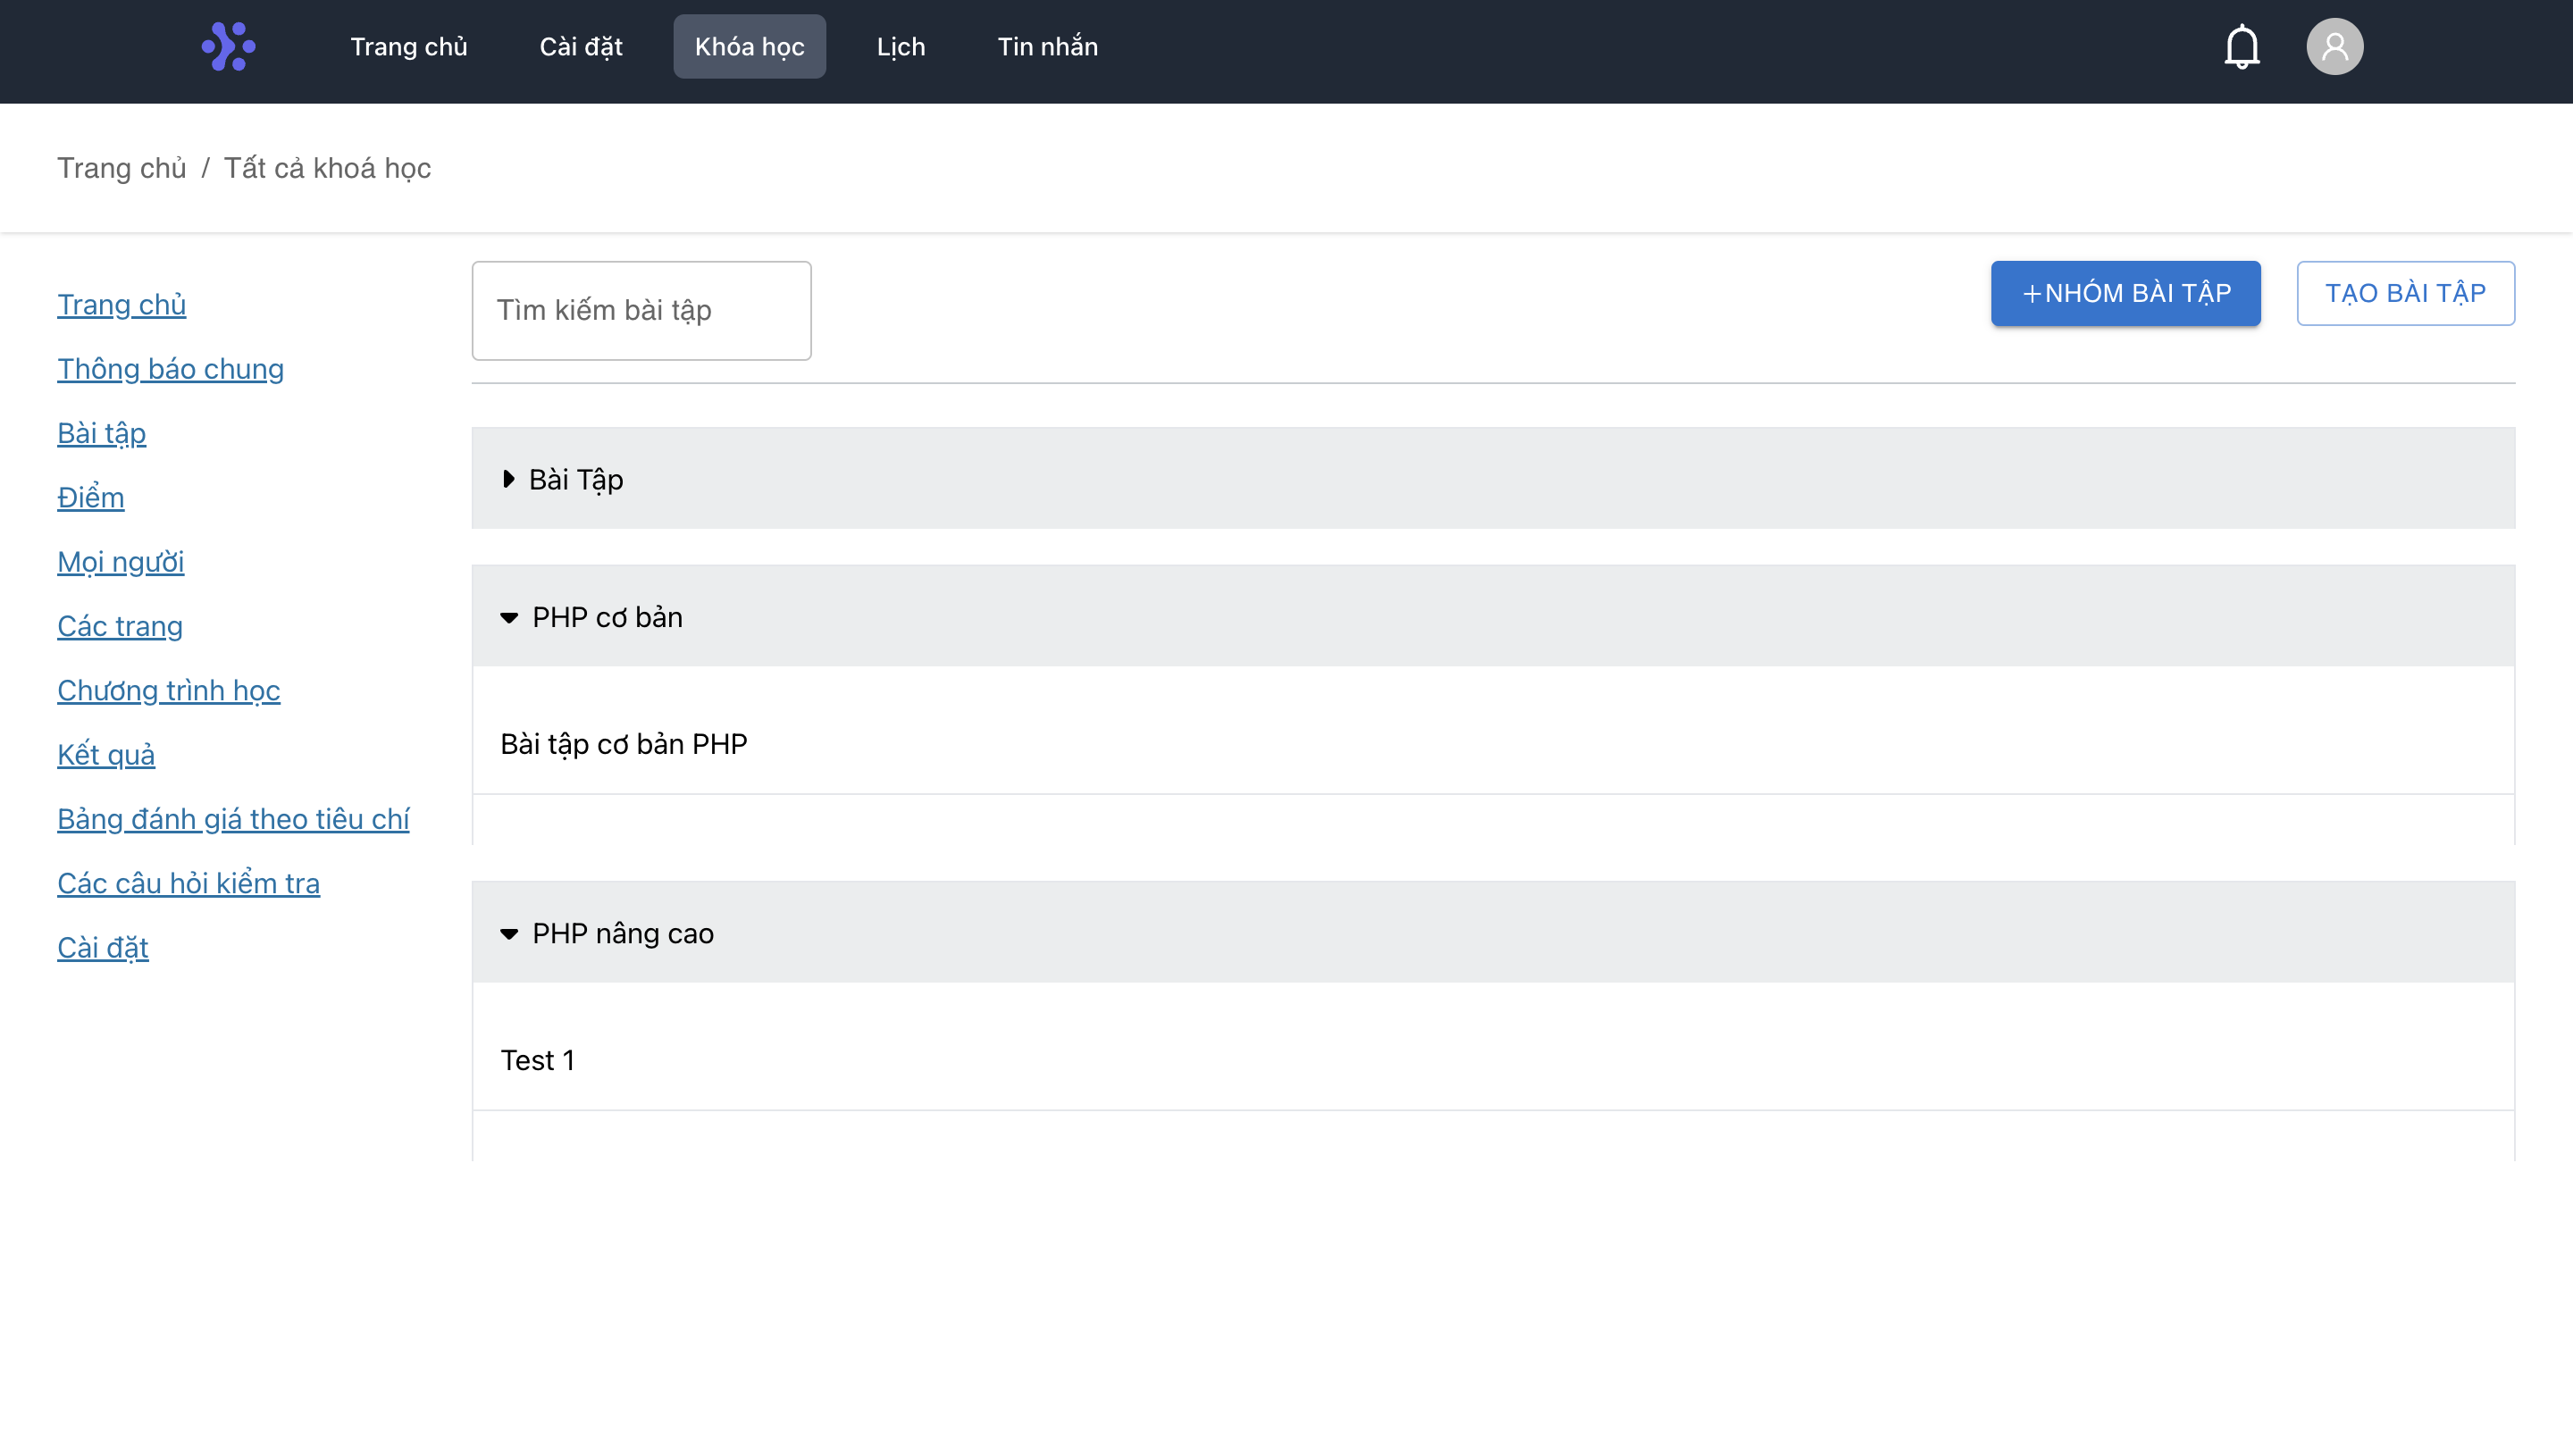
\includegraphics[width=300pt]{danh-sach-bai-tap}
            \caption{Màn hình danh sách bài tập của phần quản trị viên}
            \label{fig:danh-sach-bai-tap}
        \end{figure}

        Phần tạo nhóm của phần quản trị viên được thể hiện ở hình:
        \begin{figure}[ht!]
            \centering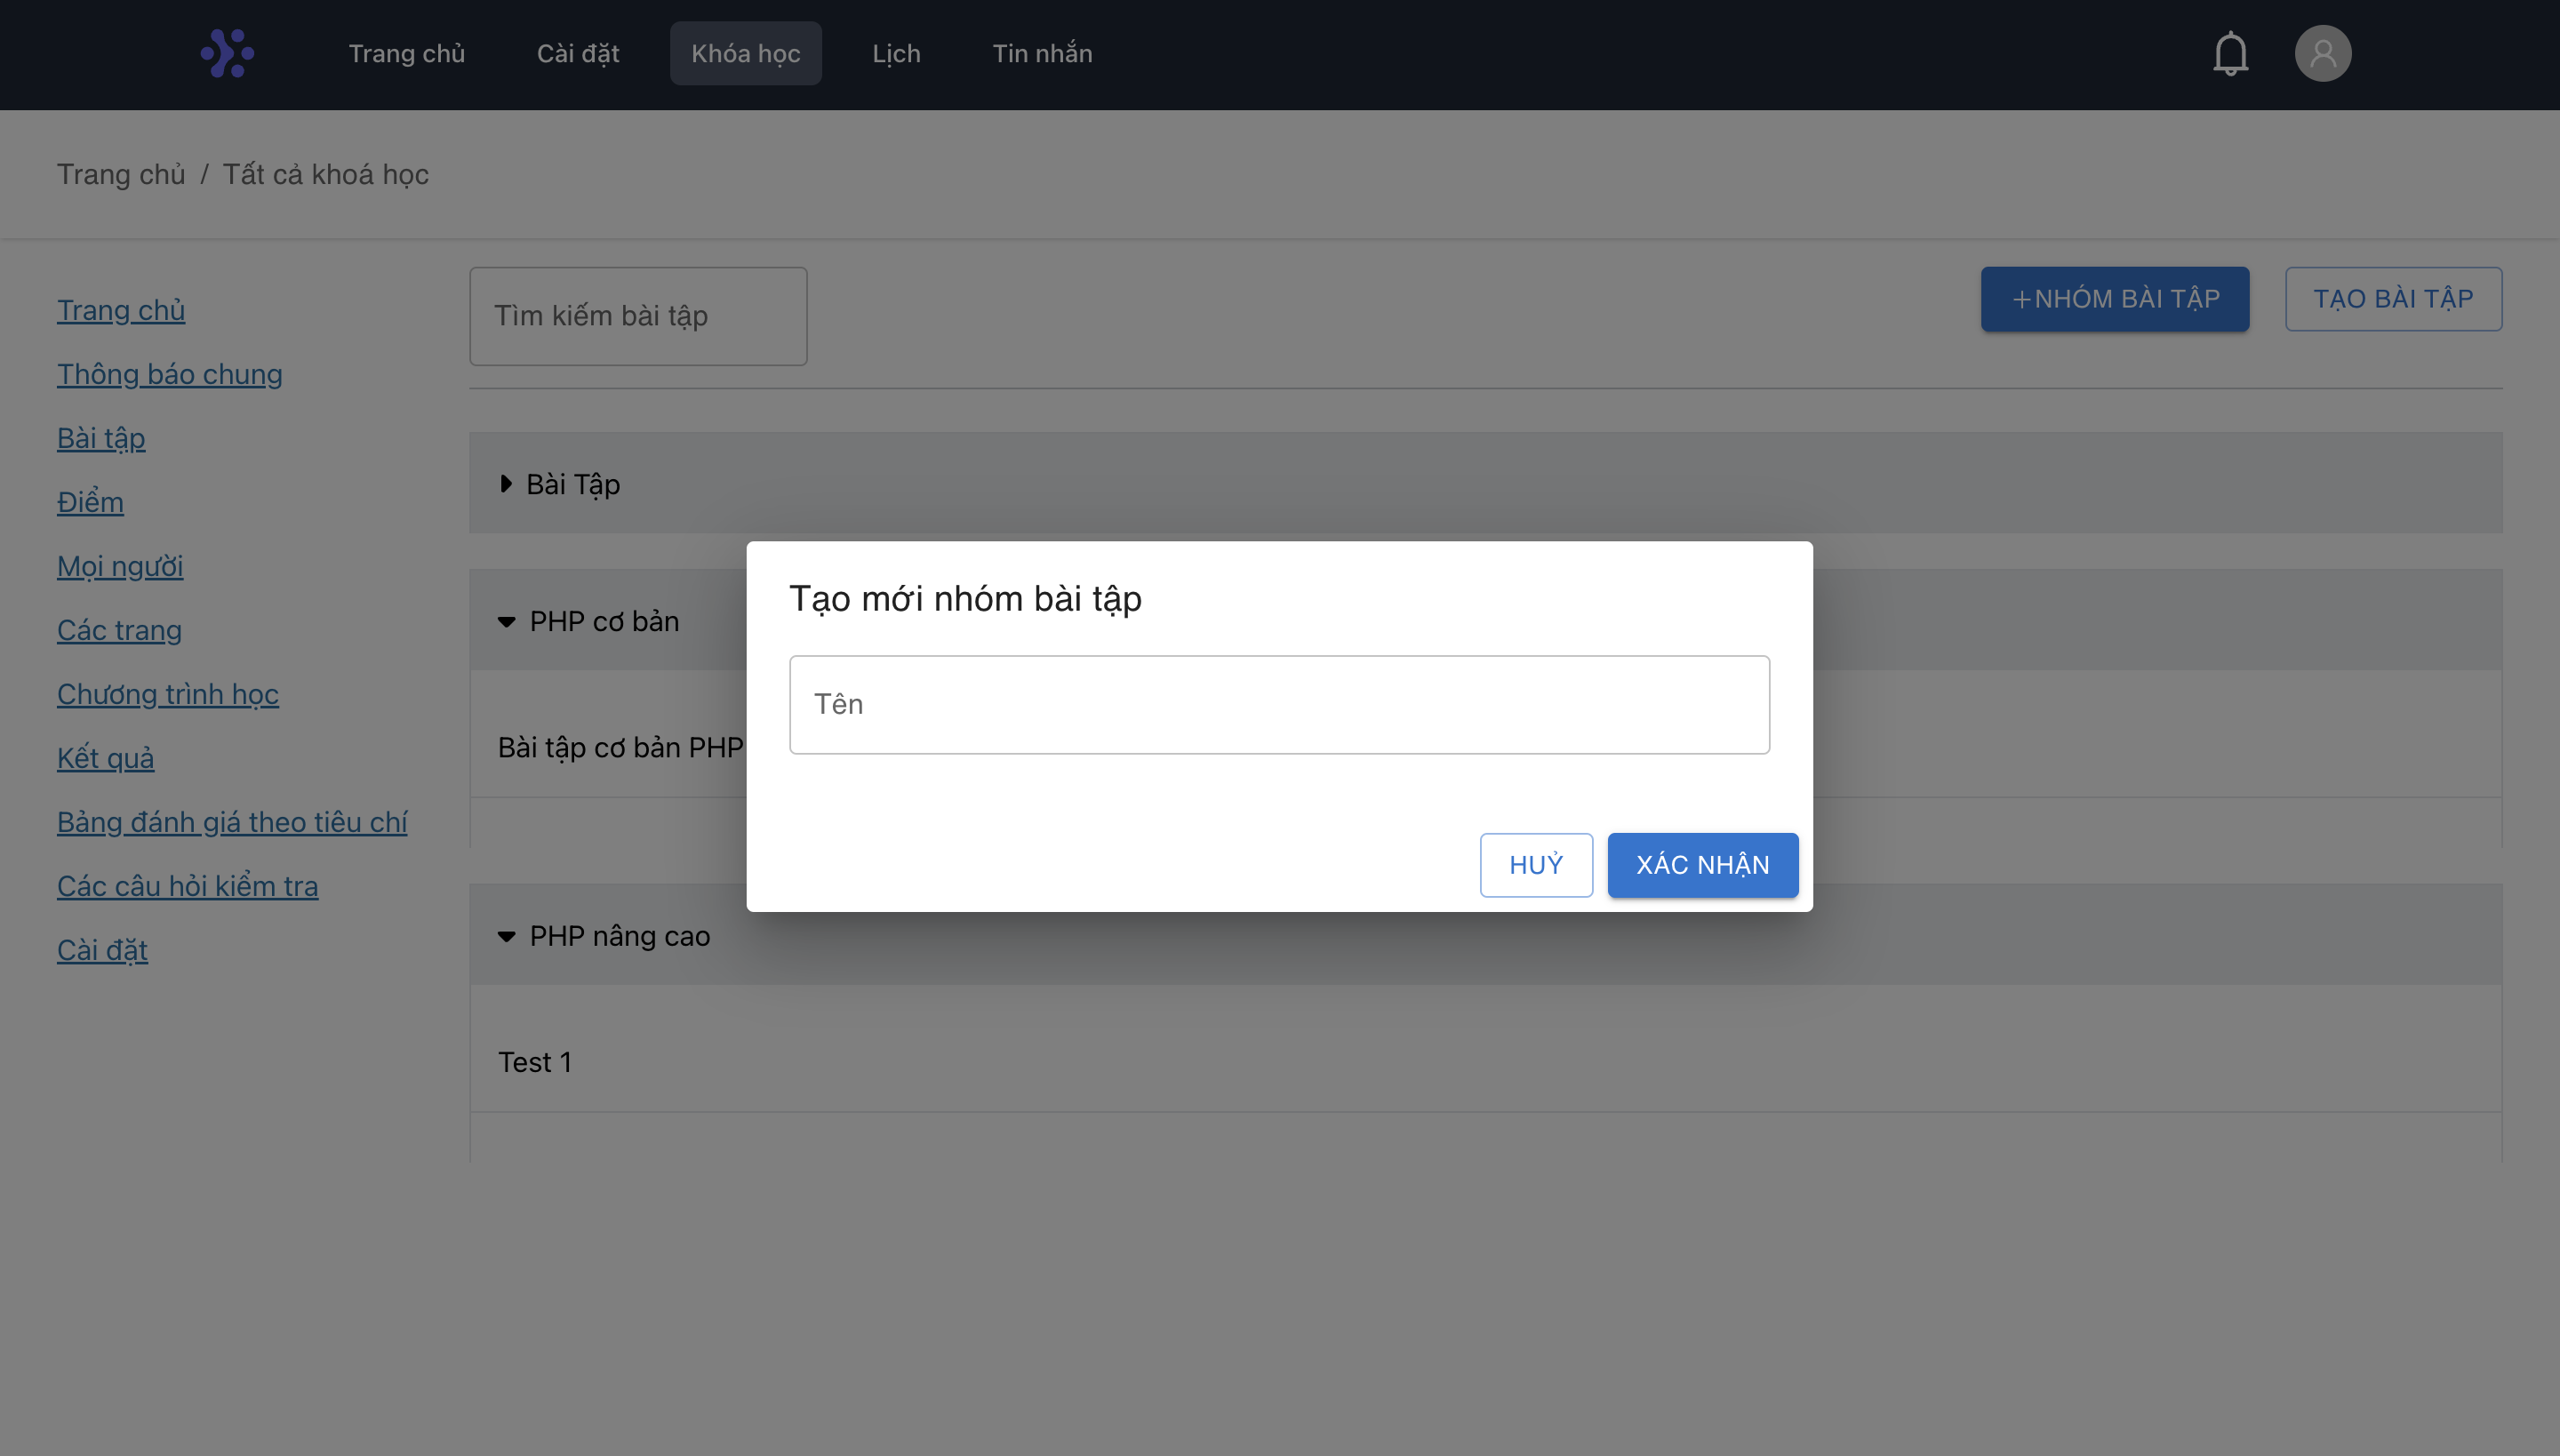
\includegraphics[width=300pt]{tao-nhom-bai-tap}
            \caption{Màn hình tạo nhóm của phần quản trị viên}
            \label{fig:tao-nhom-bai-tap}
        \end{figure}

        Phần tạo bài tập của phần quản trị viên được thể hiện ở hình:
        \begin{figure}[ht!]
            \centering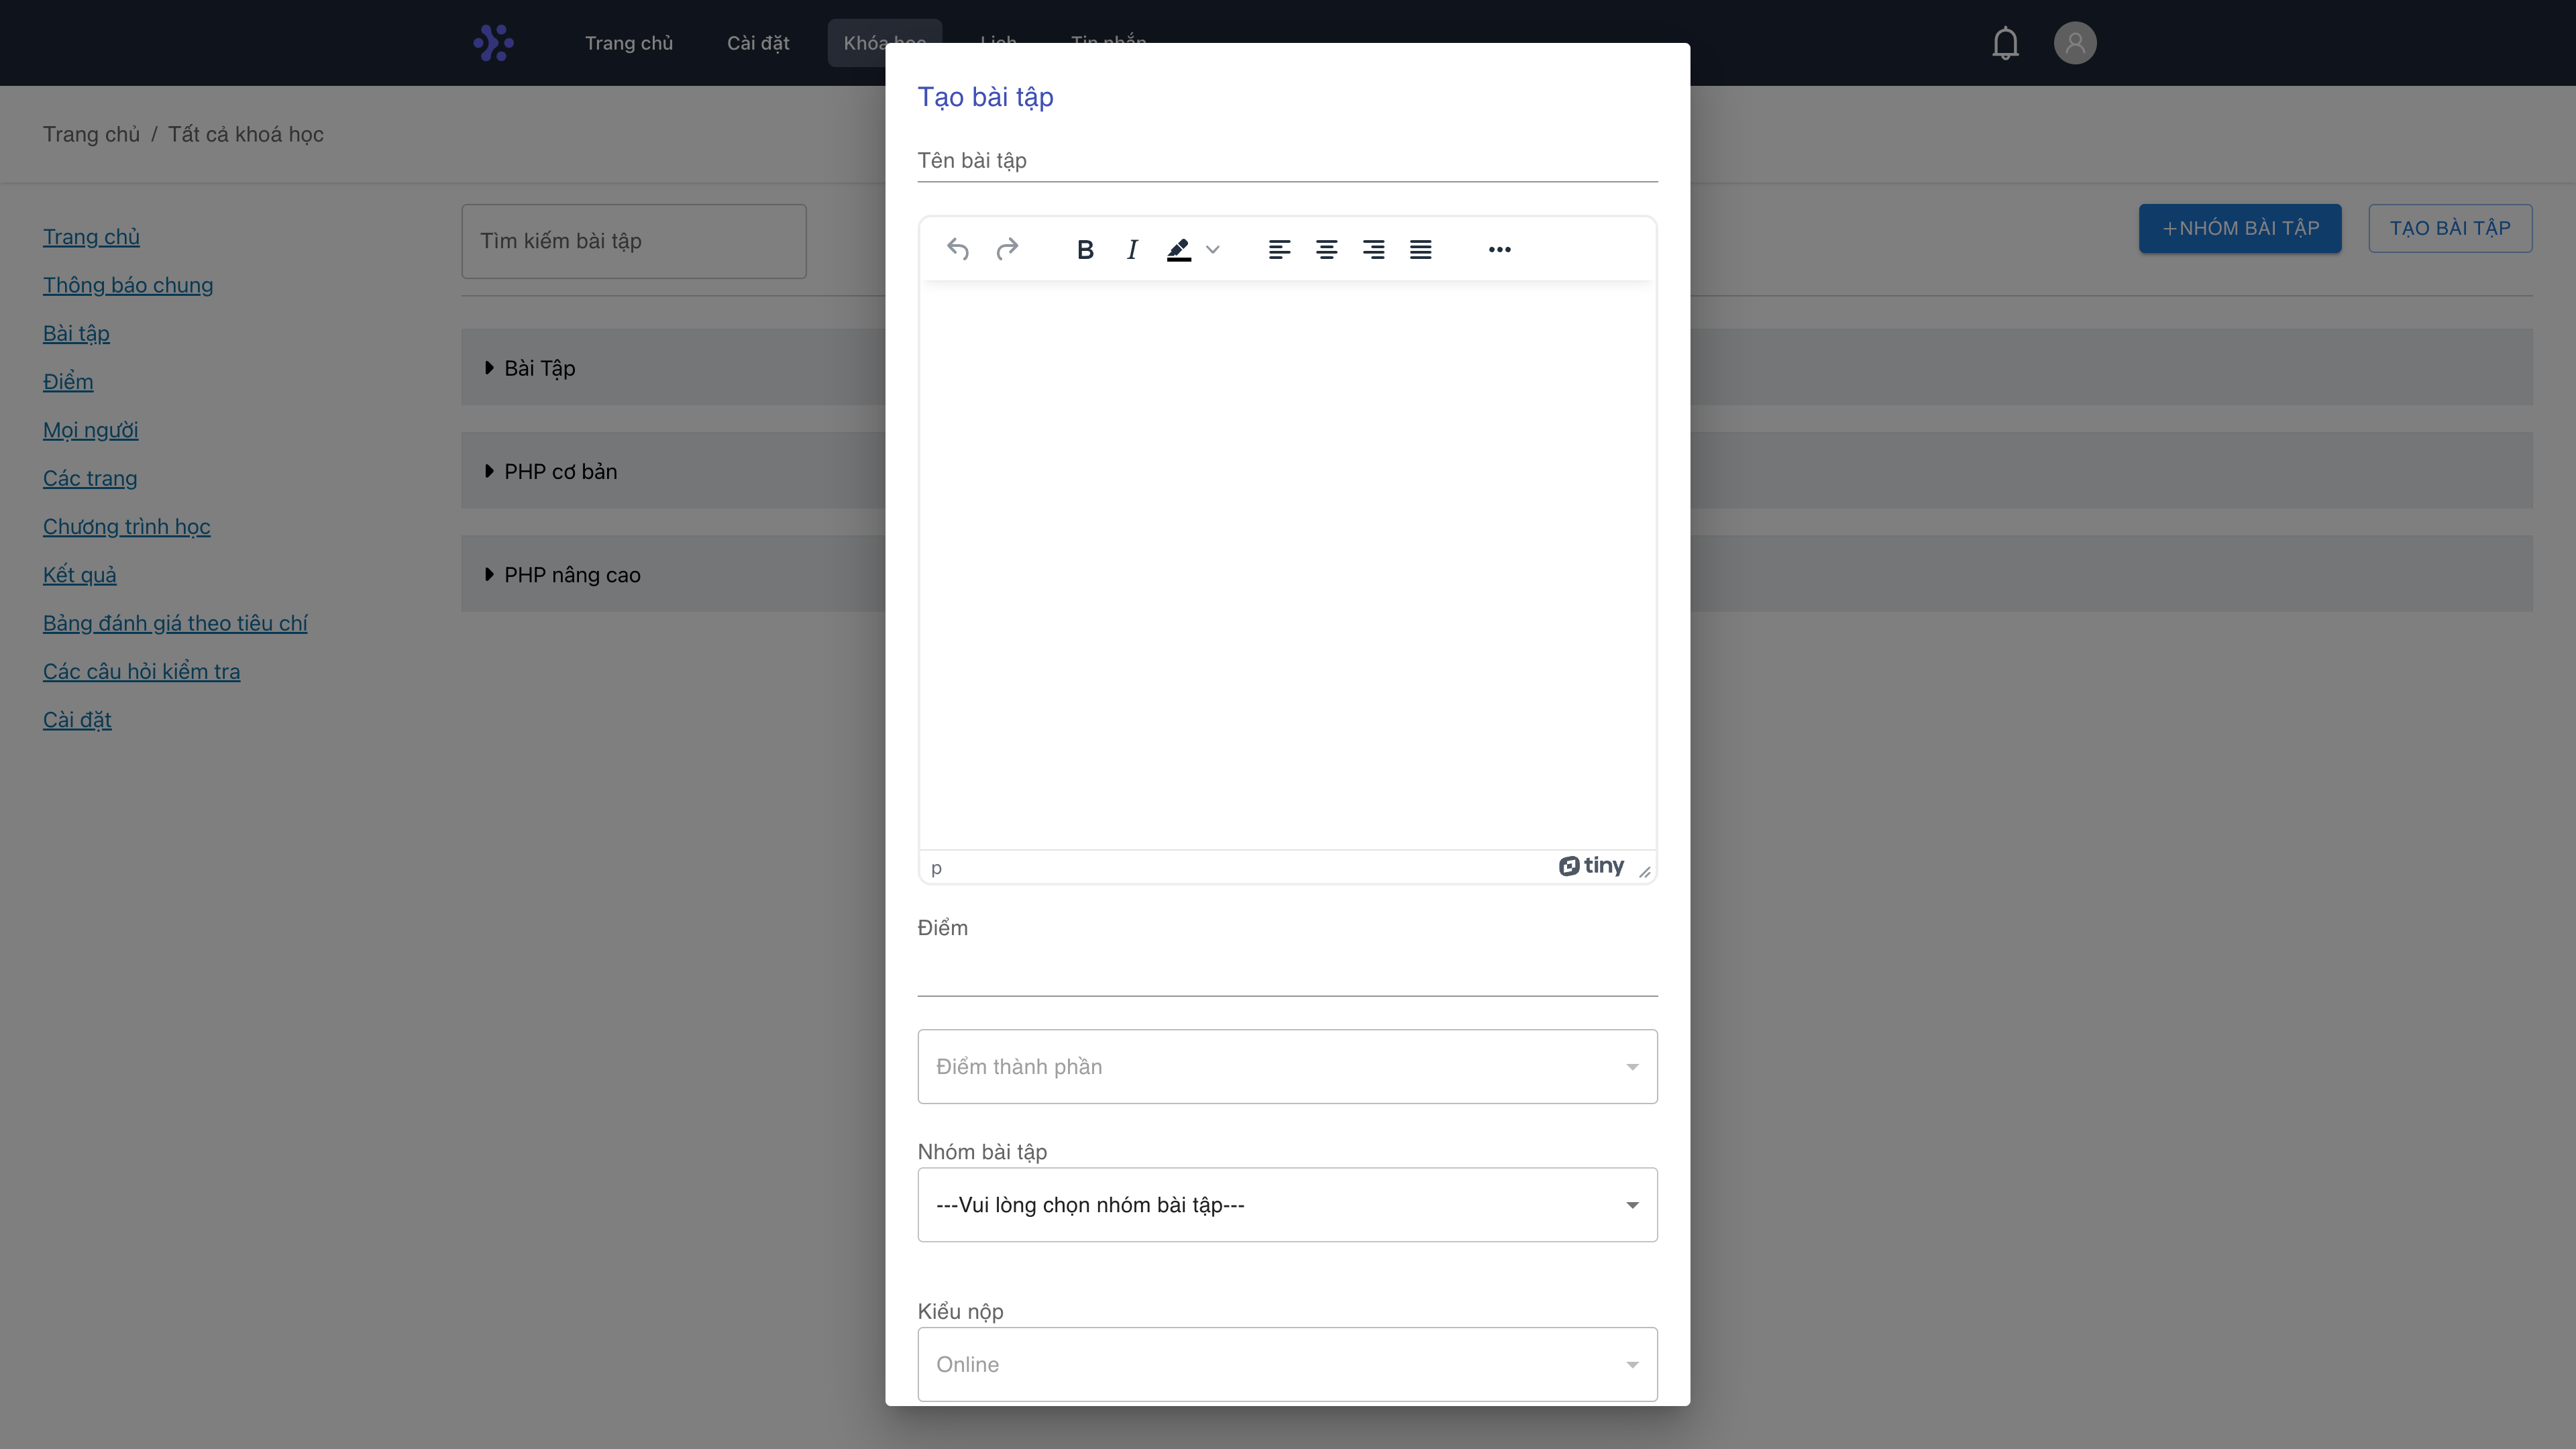
\includegraphics[width=300pt]{tao-bai-tap}
            \caption{Màn hình tạo bài tập của phần quản trị viên}
            \label{fig:tao-bai-tap}
        \end{figure}

        Phần chi tiết bài tập của phần quản trị viên được thể hiện ở hình:
        \begin{figure}[ht!]
            \centering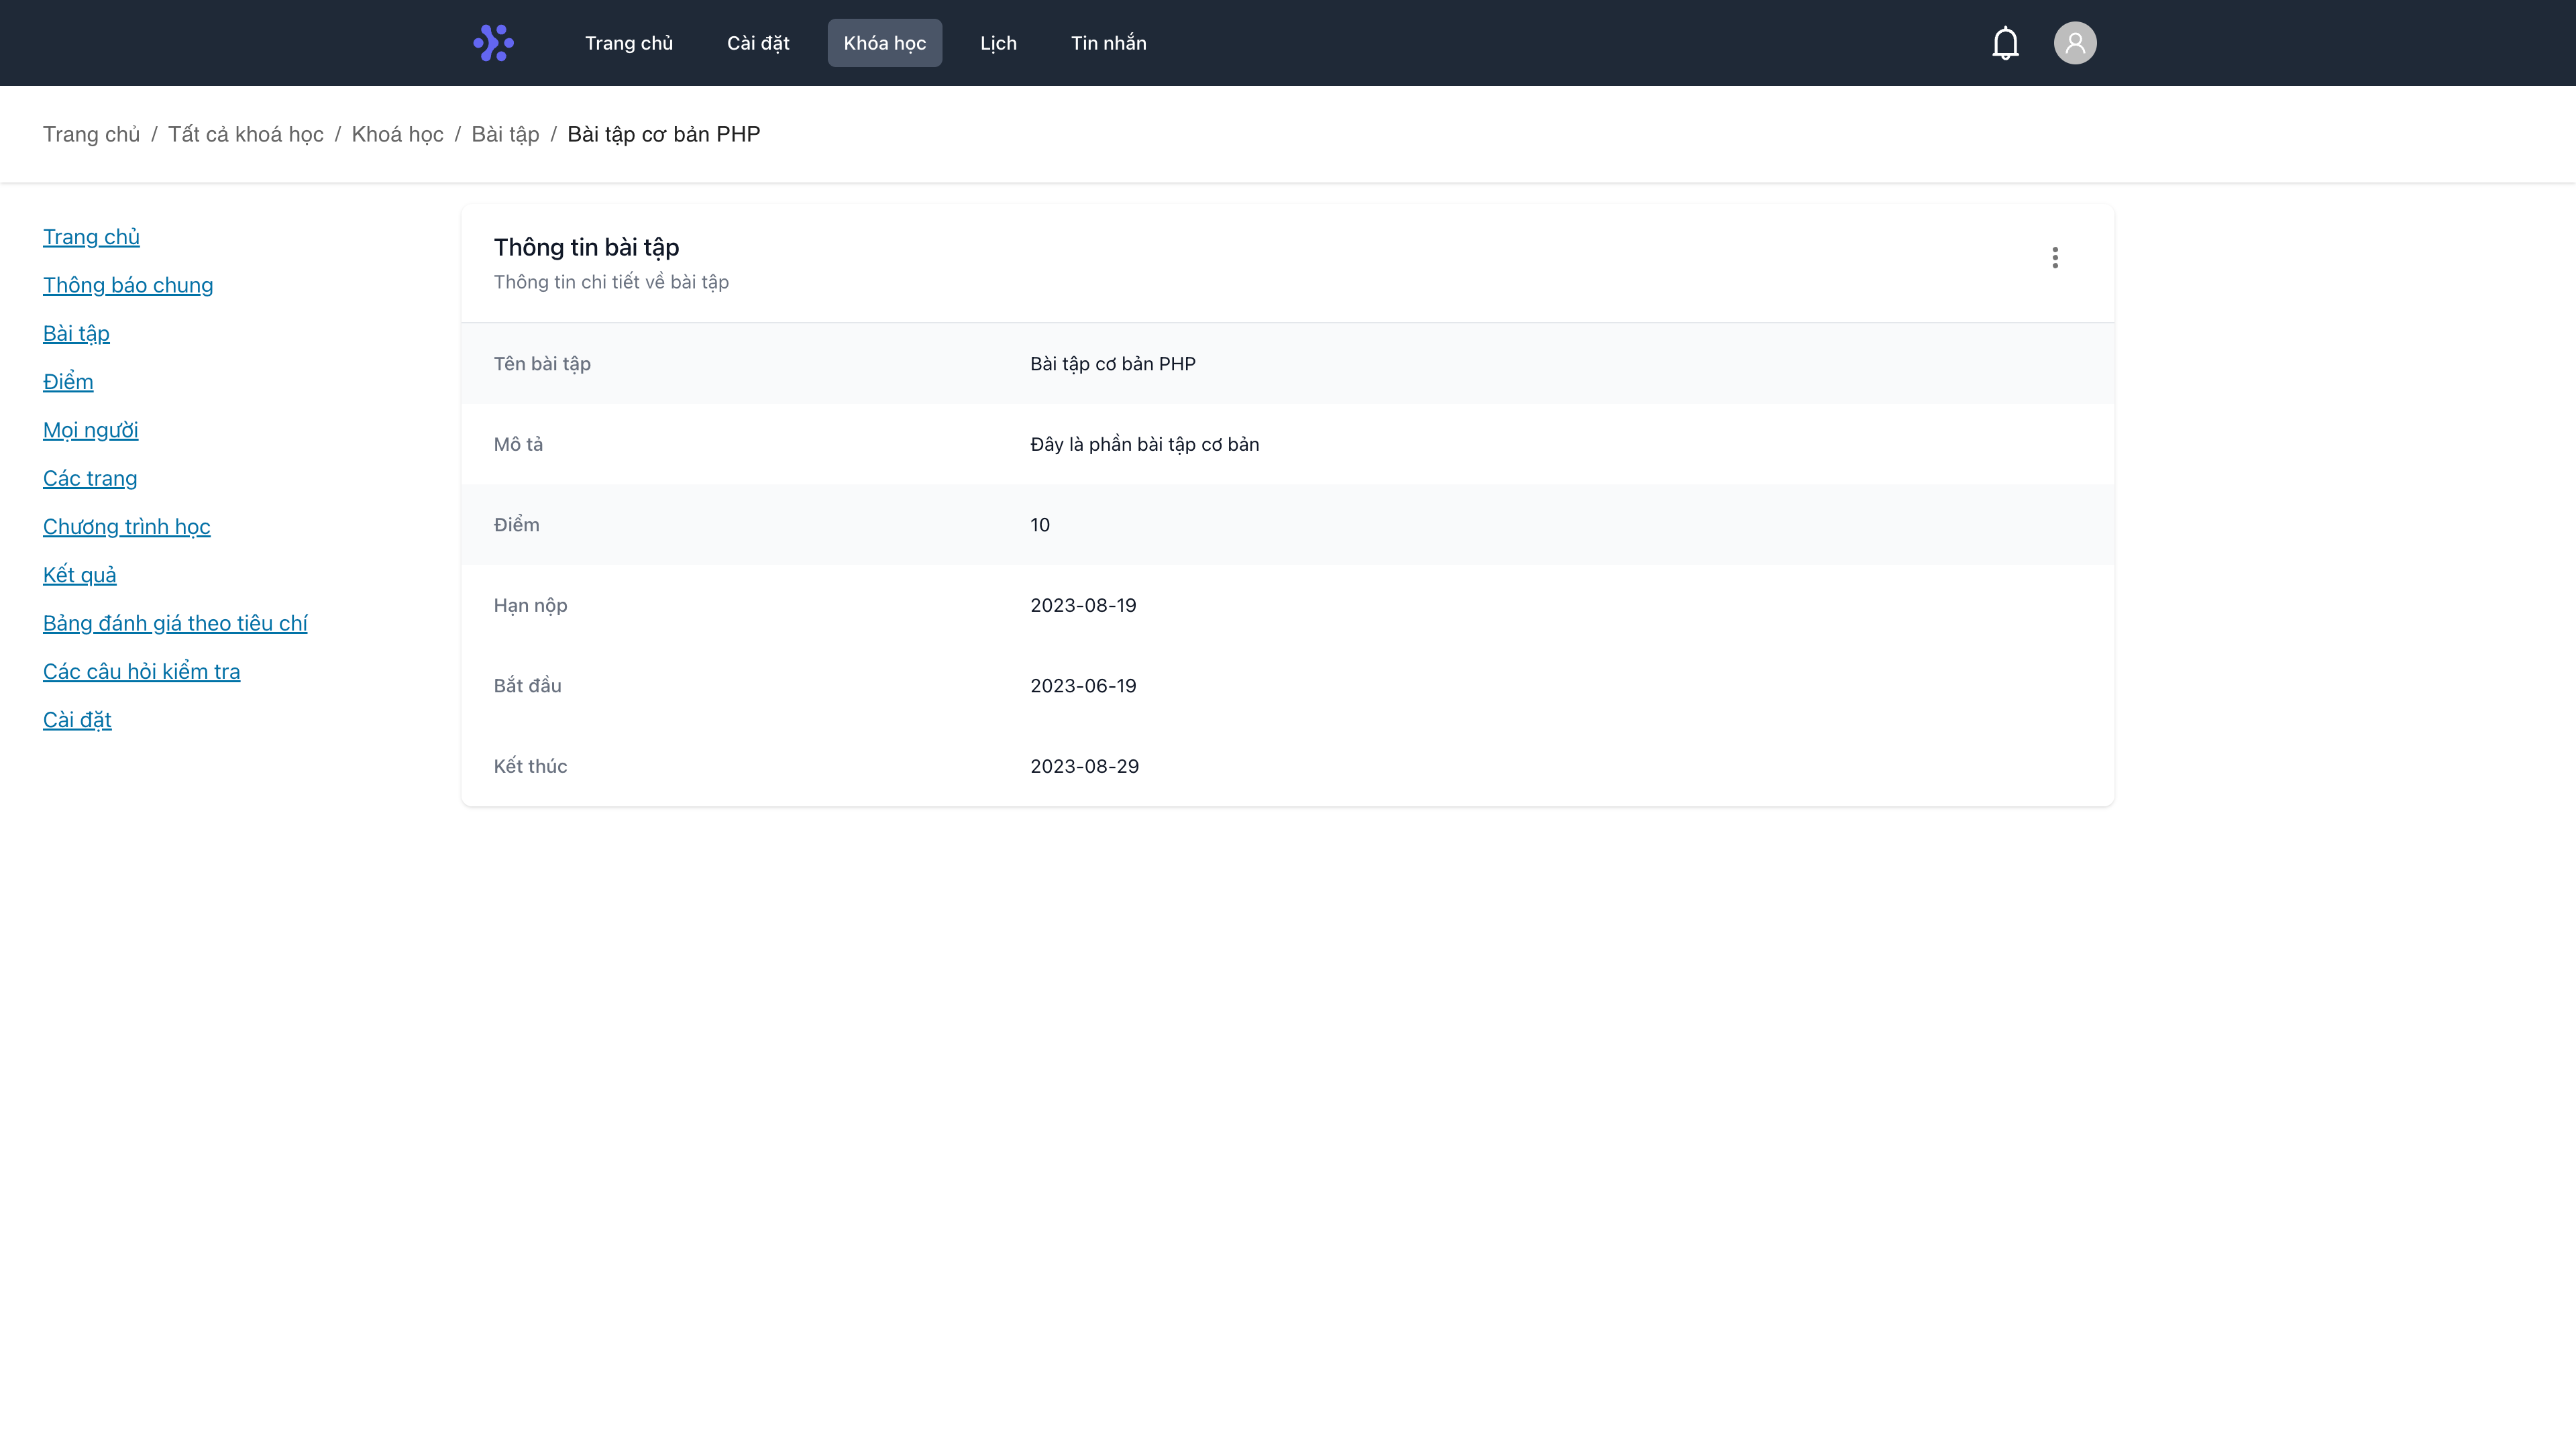
\includegraphics[width=300pt]{chi-tiet-bai-tap}
            \caption{Màn hình chi tiết bài tập của phần quản trị viên}
            \label{fig:chi-tiet-bai-tap}
        \end{figure}

        Phần chỉnh sửa bài tập của phần quản trị viên được thể hiện ở hình:
        \begin{figure}[ht!]
            \centering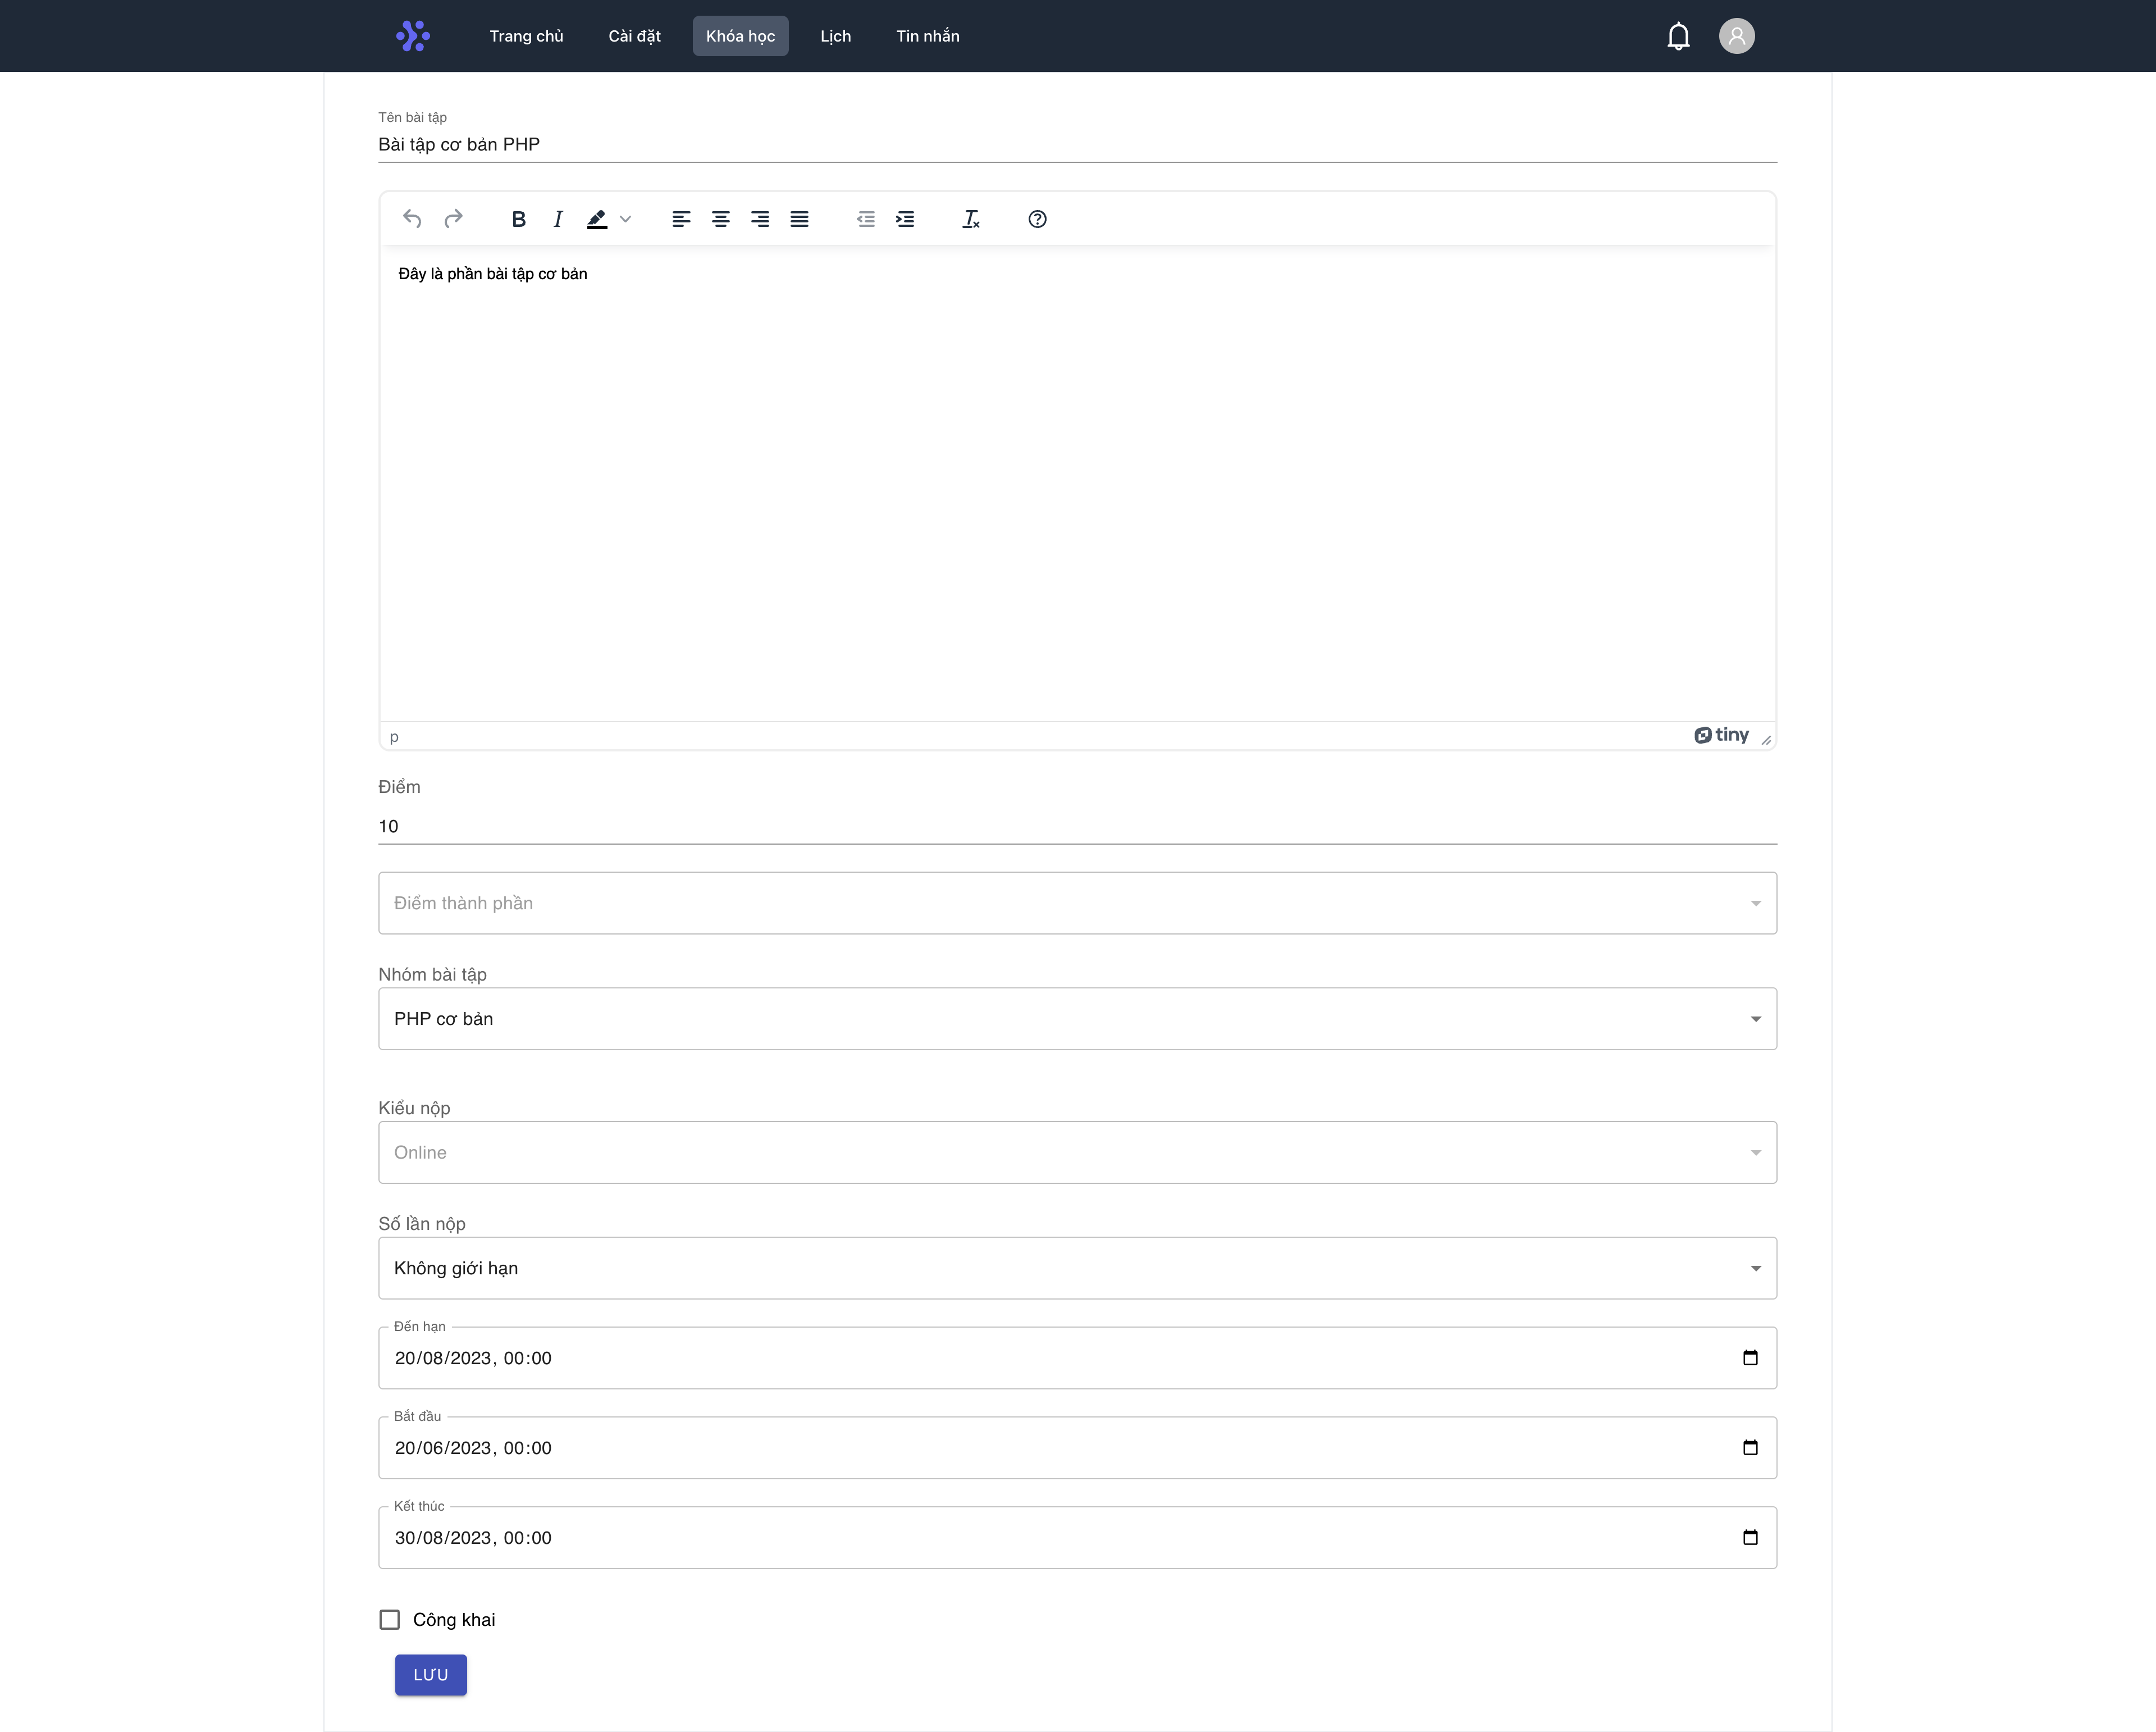
\includegraphics[width=300pt]{chinh-sua-bai-tap}
            \caption{Màn hình chỉnh sửa bài tập của phần quản trị viên}
            \label{fig:chinh-sua-bai-tap}
        \end{figure}

        Phần câu hỏi kiểm tra của phần quản trị viên được thể hiện ở hình:
        \begin{figure}[ht!]
            \centering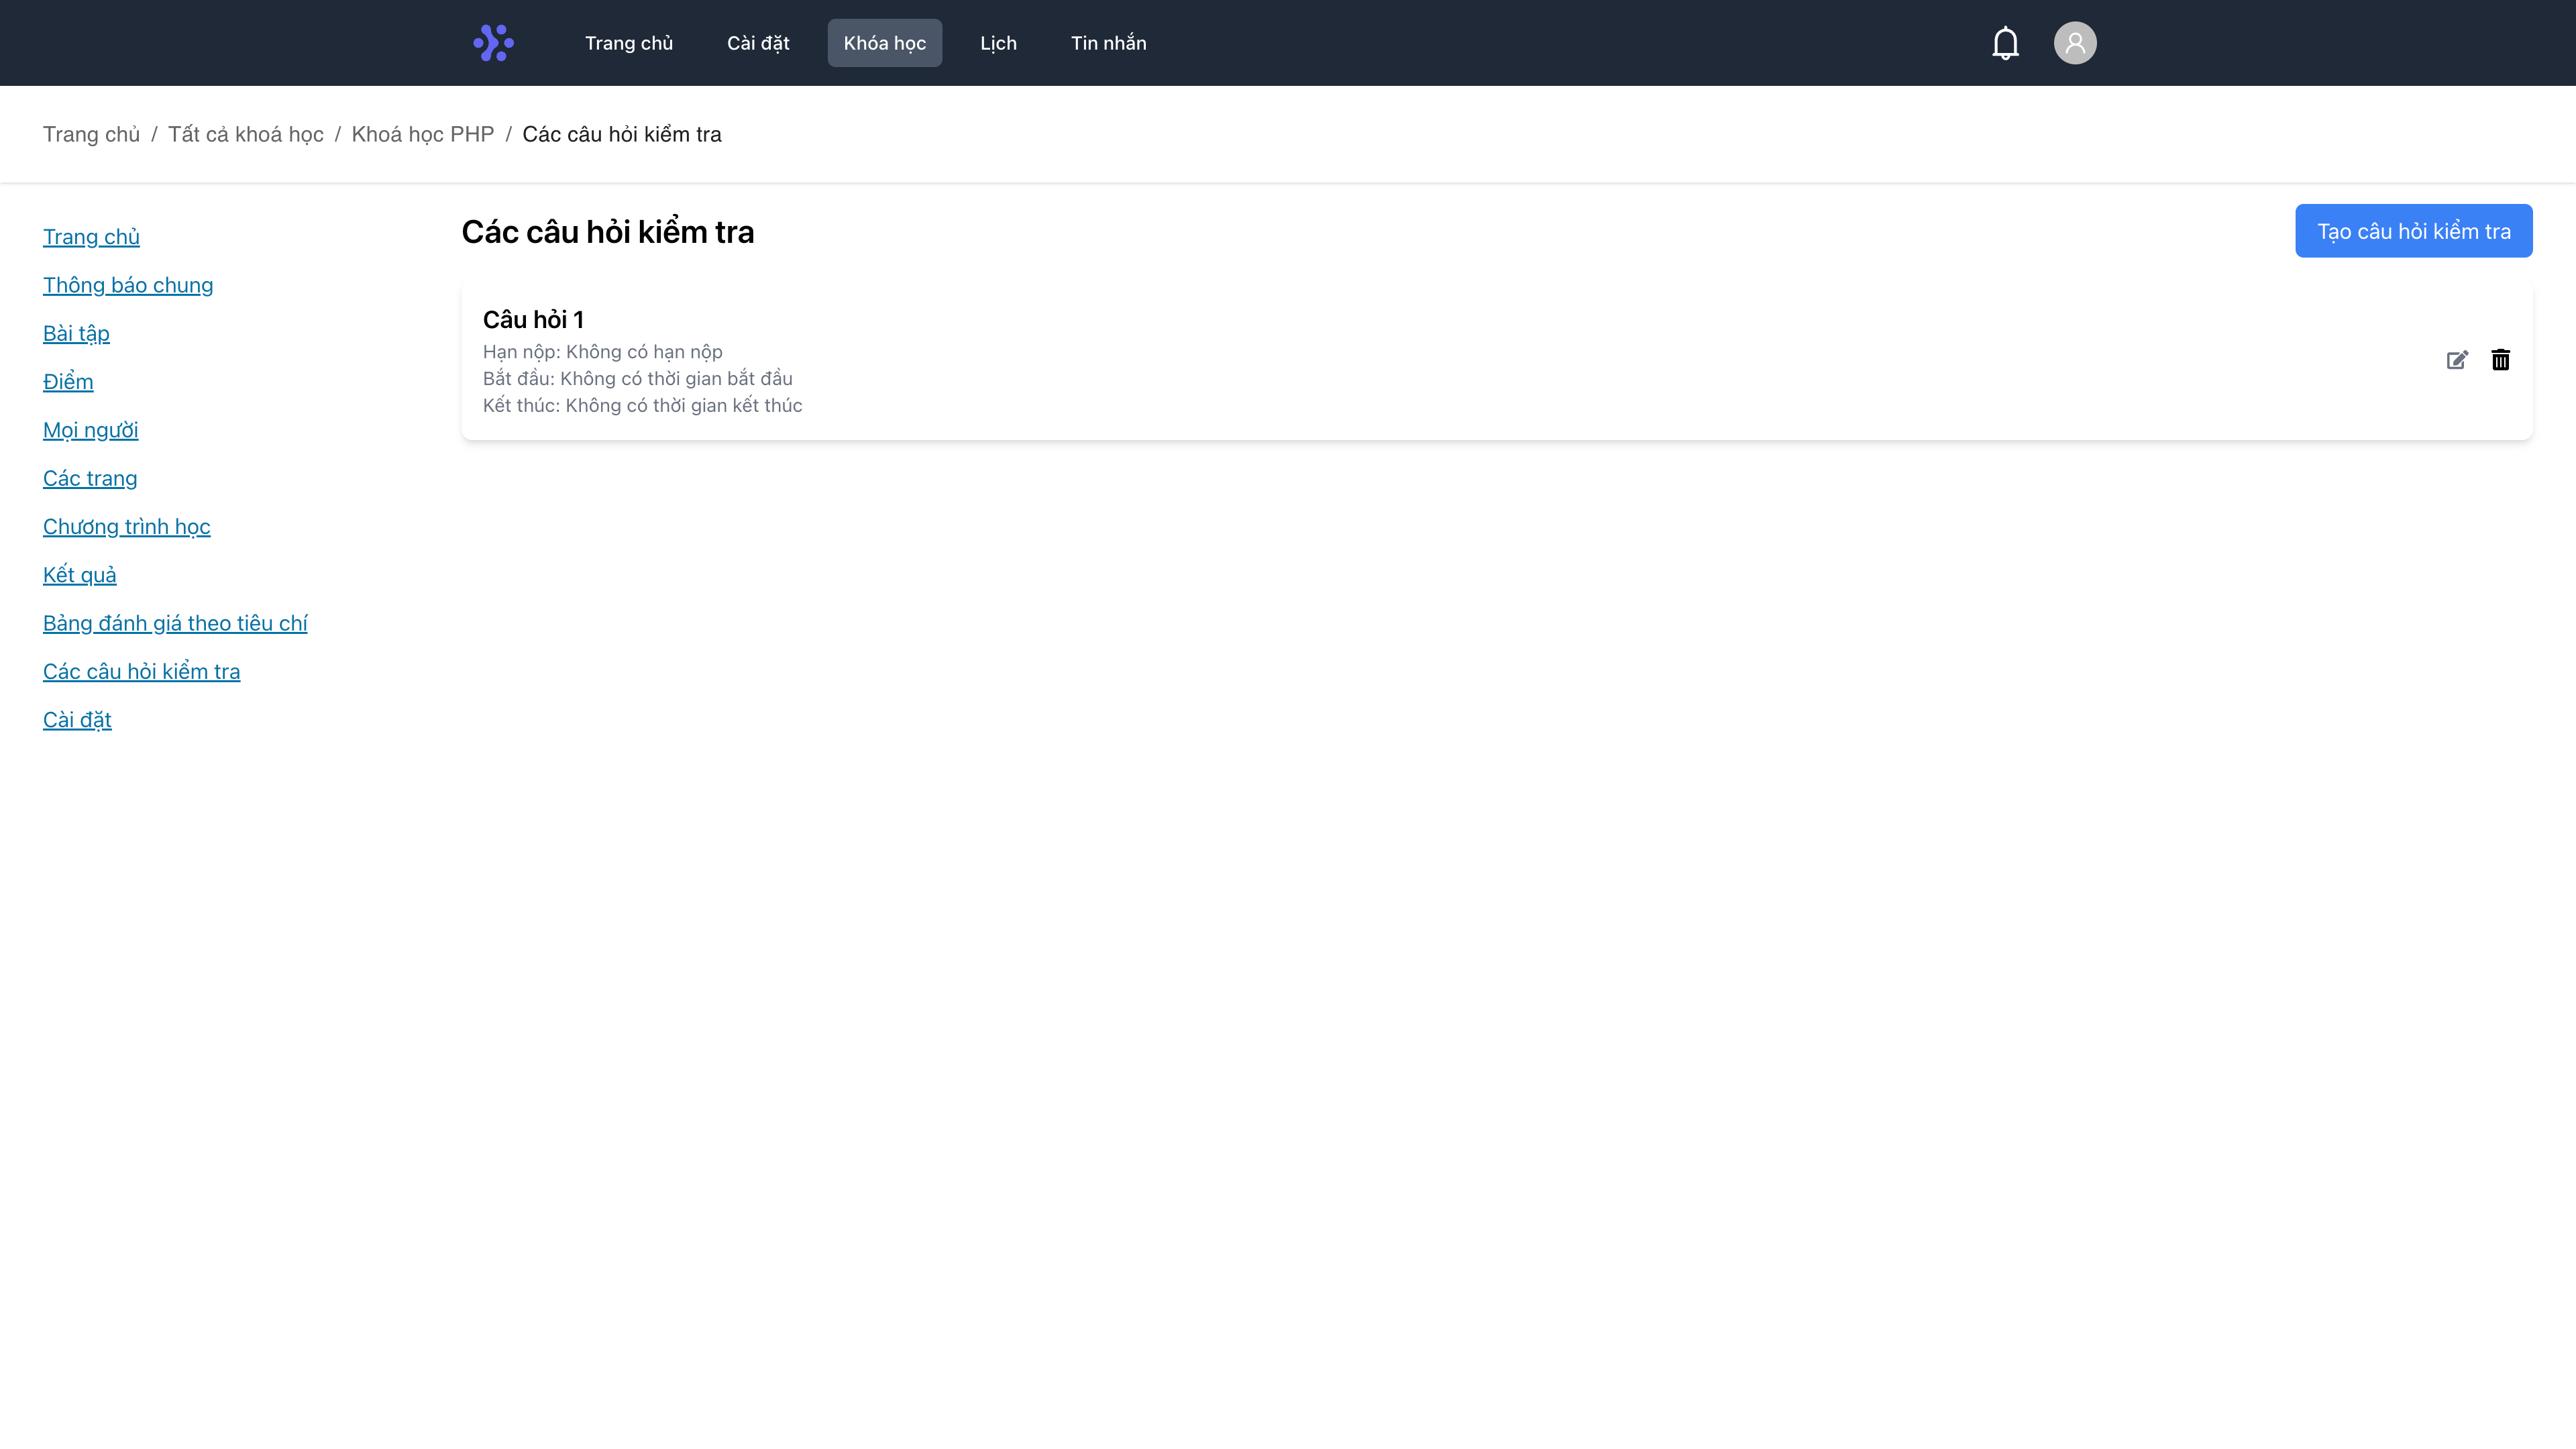
\includegraphics[width=300pt]{cau-hoi-kiem-tra}
            \caption{Màn hình câu hỏi kiểm tra của phần quản trị viên}
            \label{fig:cau-hoi-kiem-tra}
        \end{figure}

        Phần tạo câu hỏi kiểm tra của phần quản trị viên được thể hiện ở hình:
        \begin{figure}[ht!]
            \centering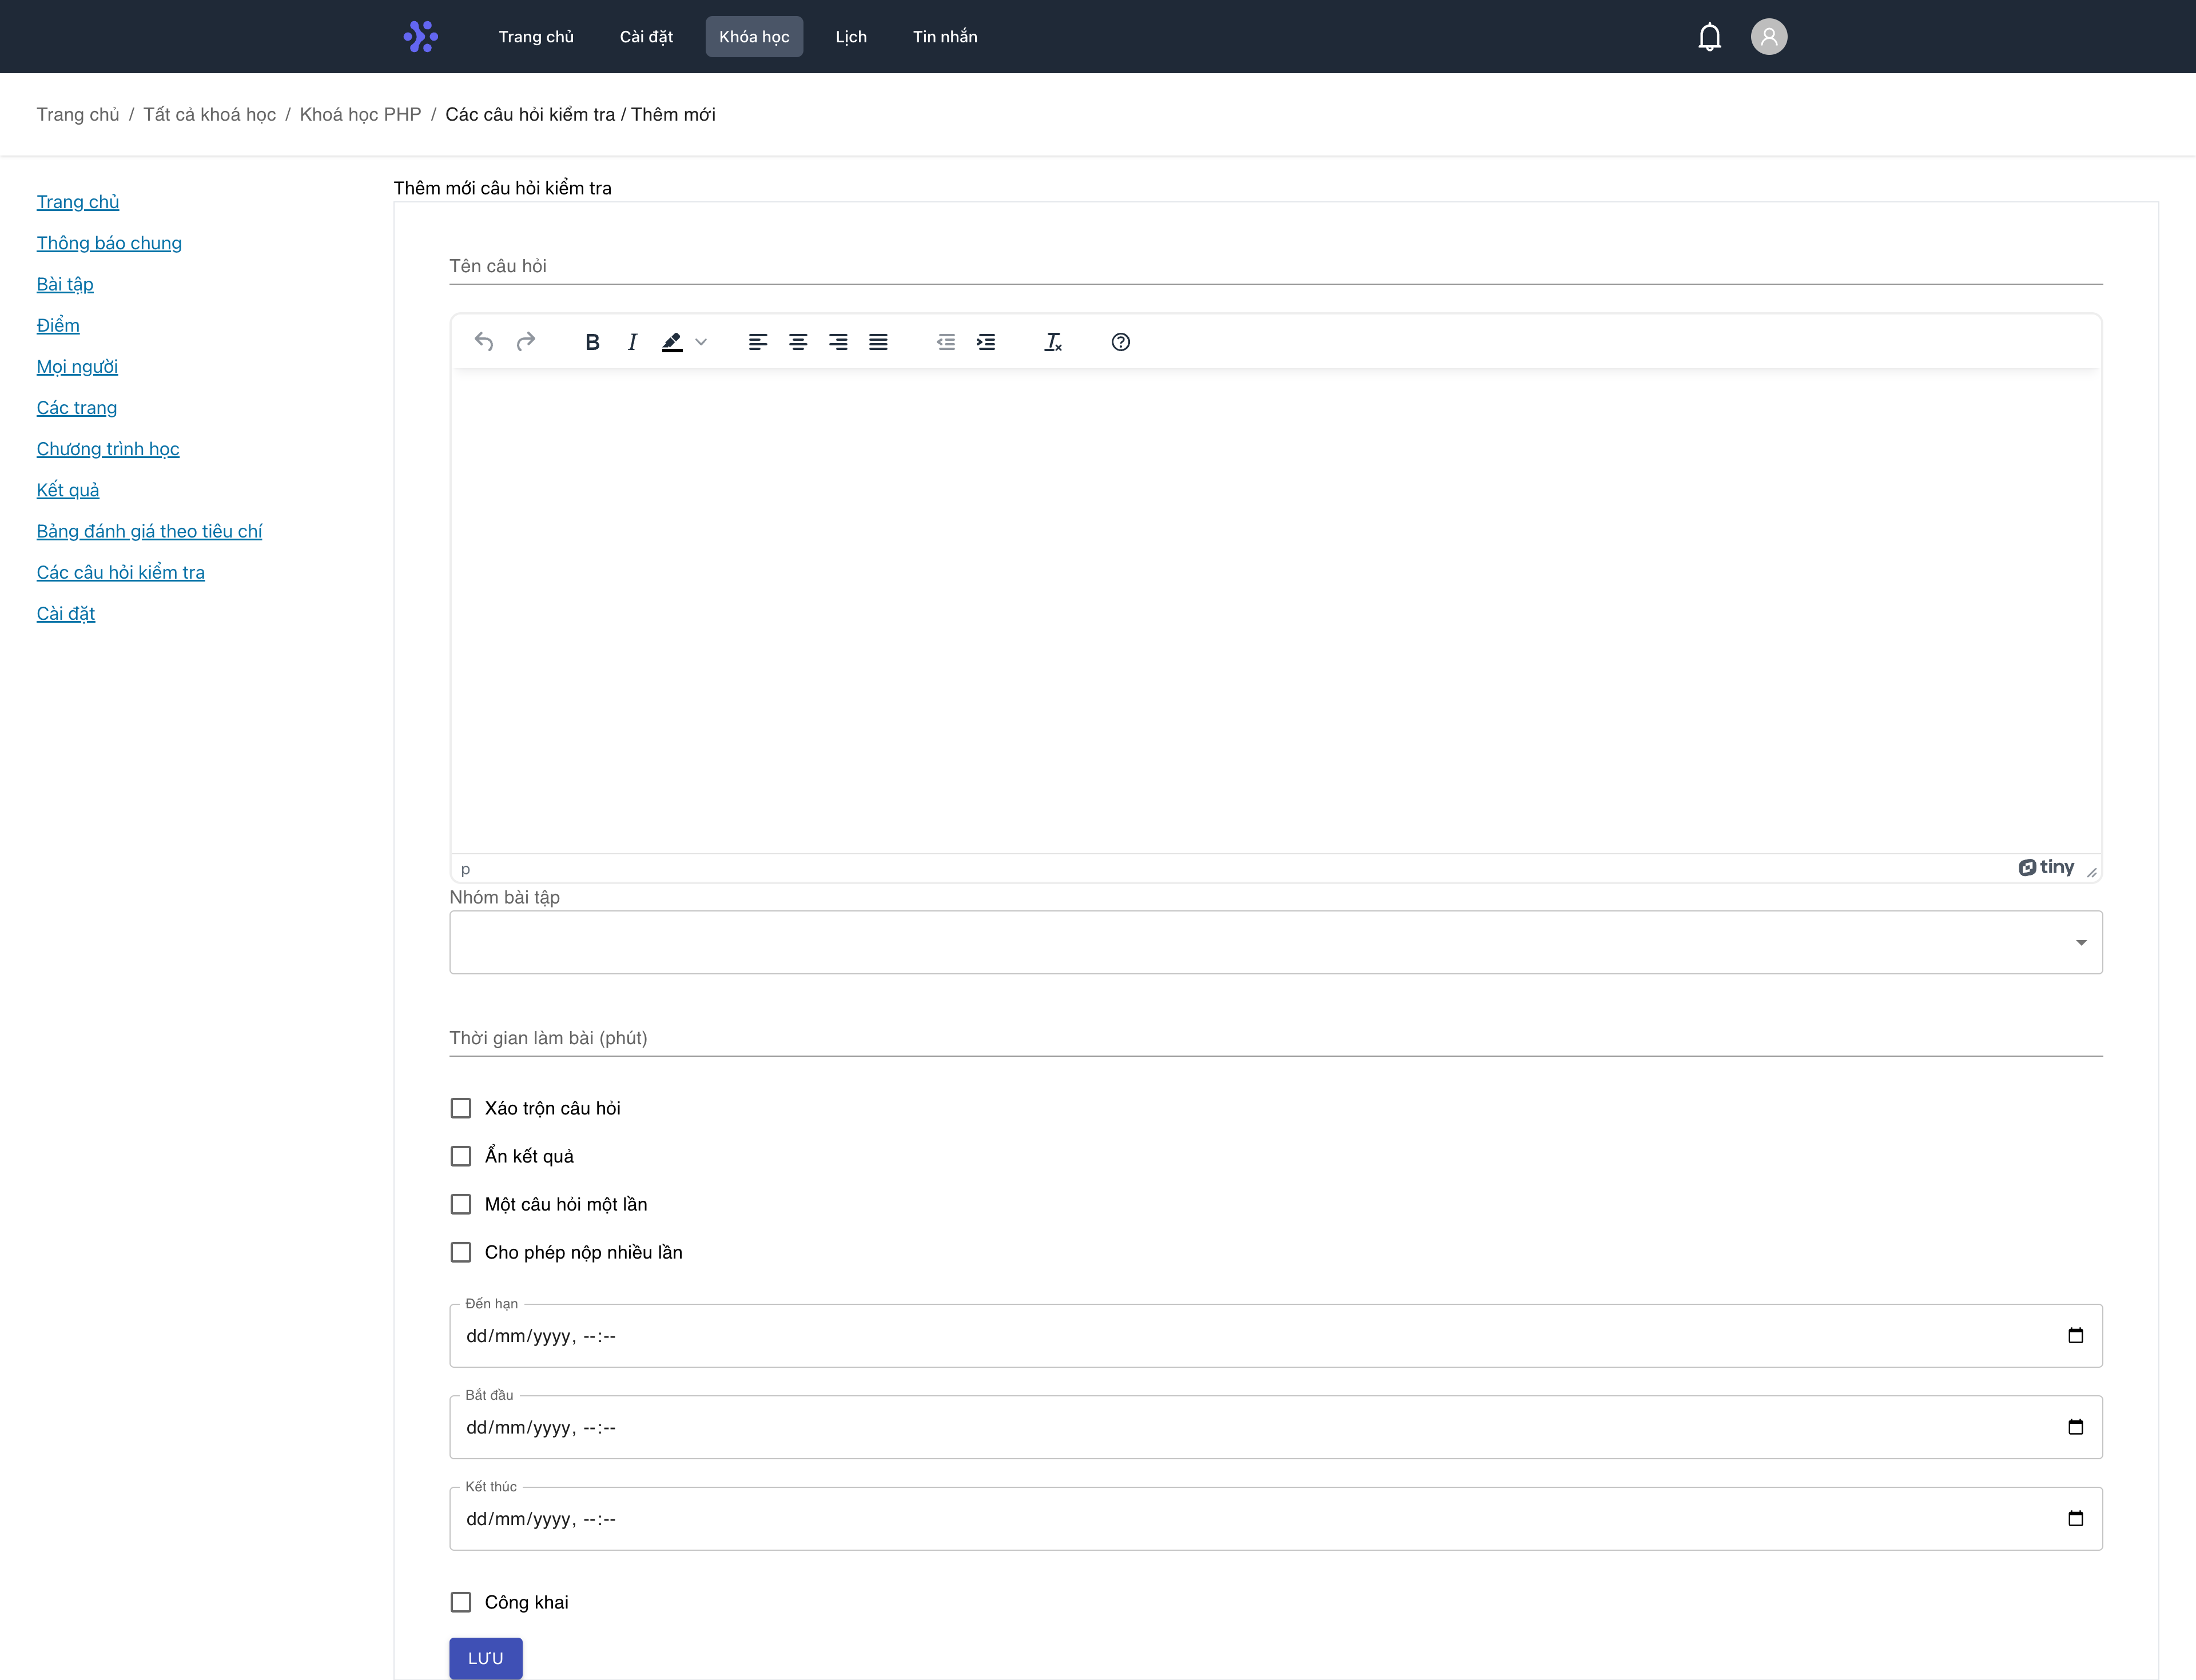
\includegraphics[width=300pt]{tao-cau-hoi-kiem-tra}
            \caption{Màn hình tạo câu hỏi kiểm tra của phần quản trị viên}
            \label{fig:tao-cau-hoi-kiem-tra}
        \end{figure}

        Phần chỉnh sửa câu hỏi kiểm tra của phần quản trị viên được thể hiện ở hình:
        \begin{figure}[ht!]
            \centering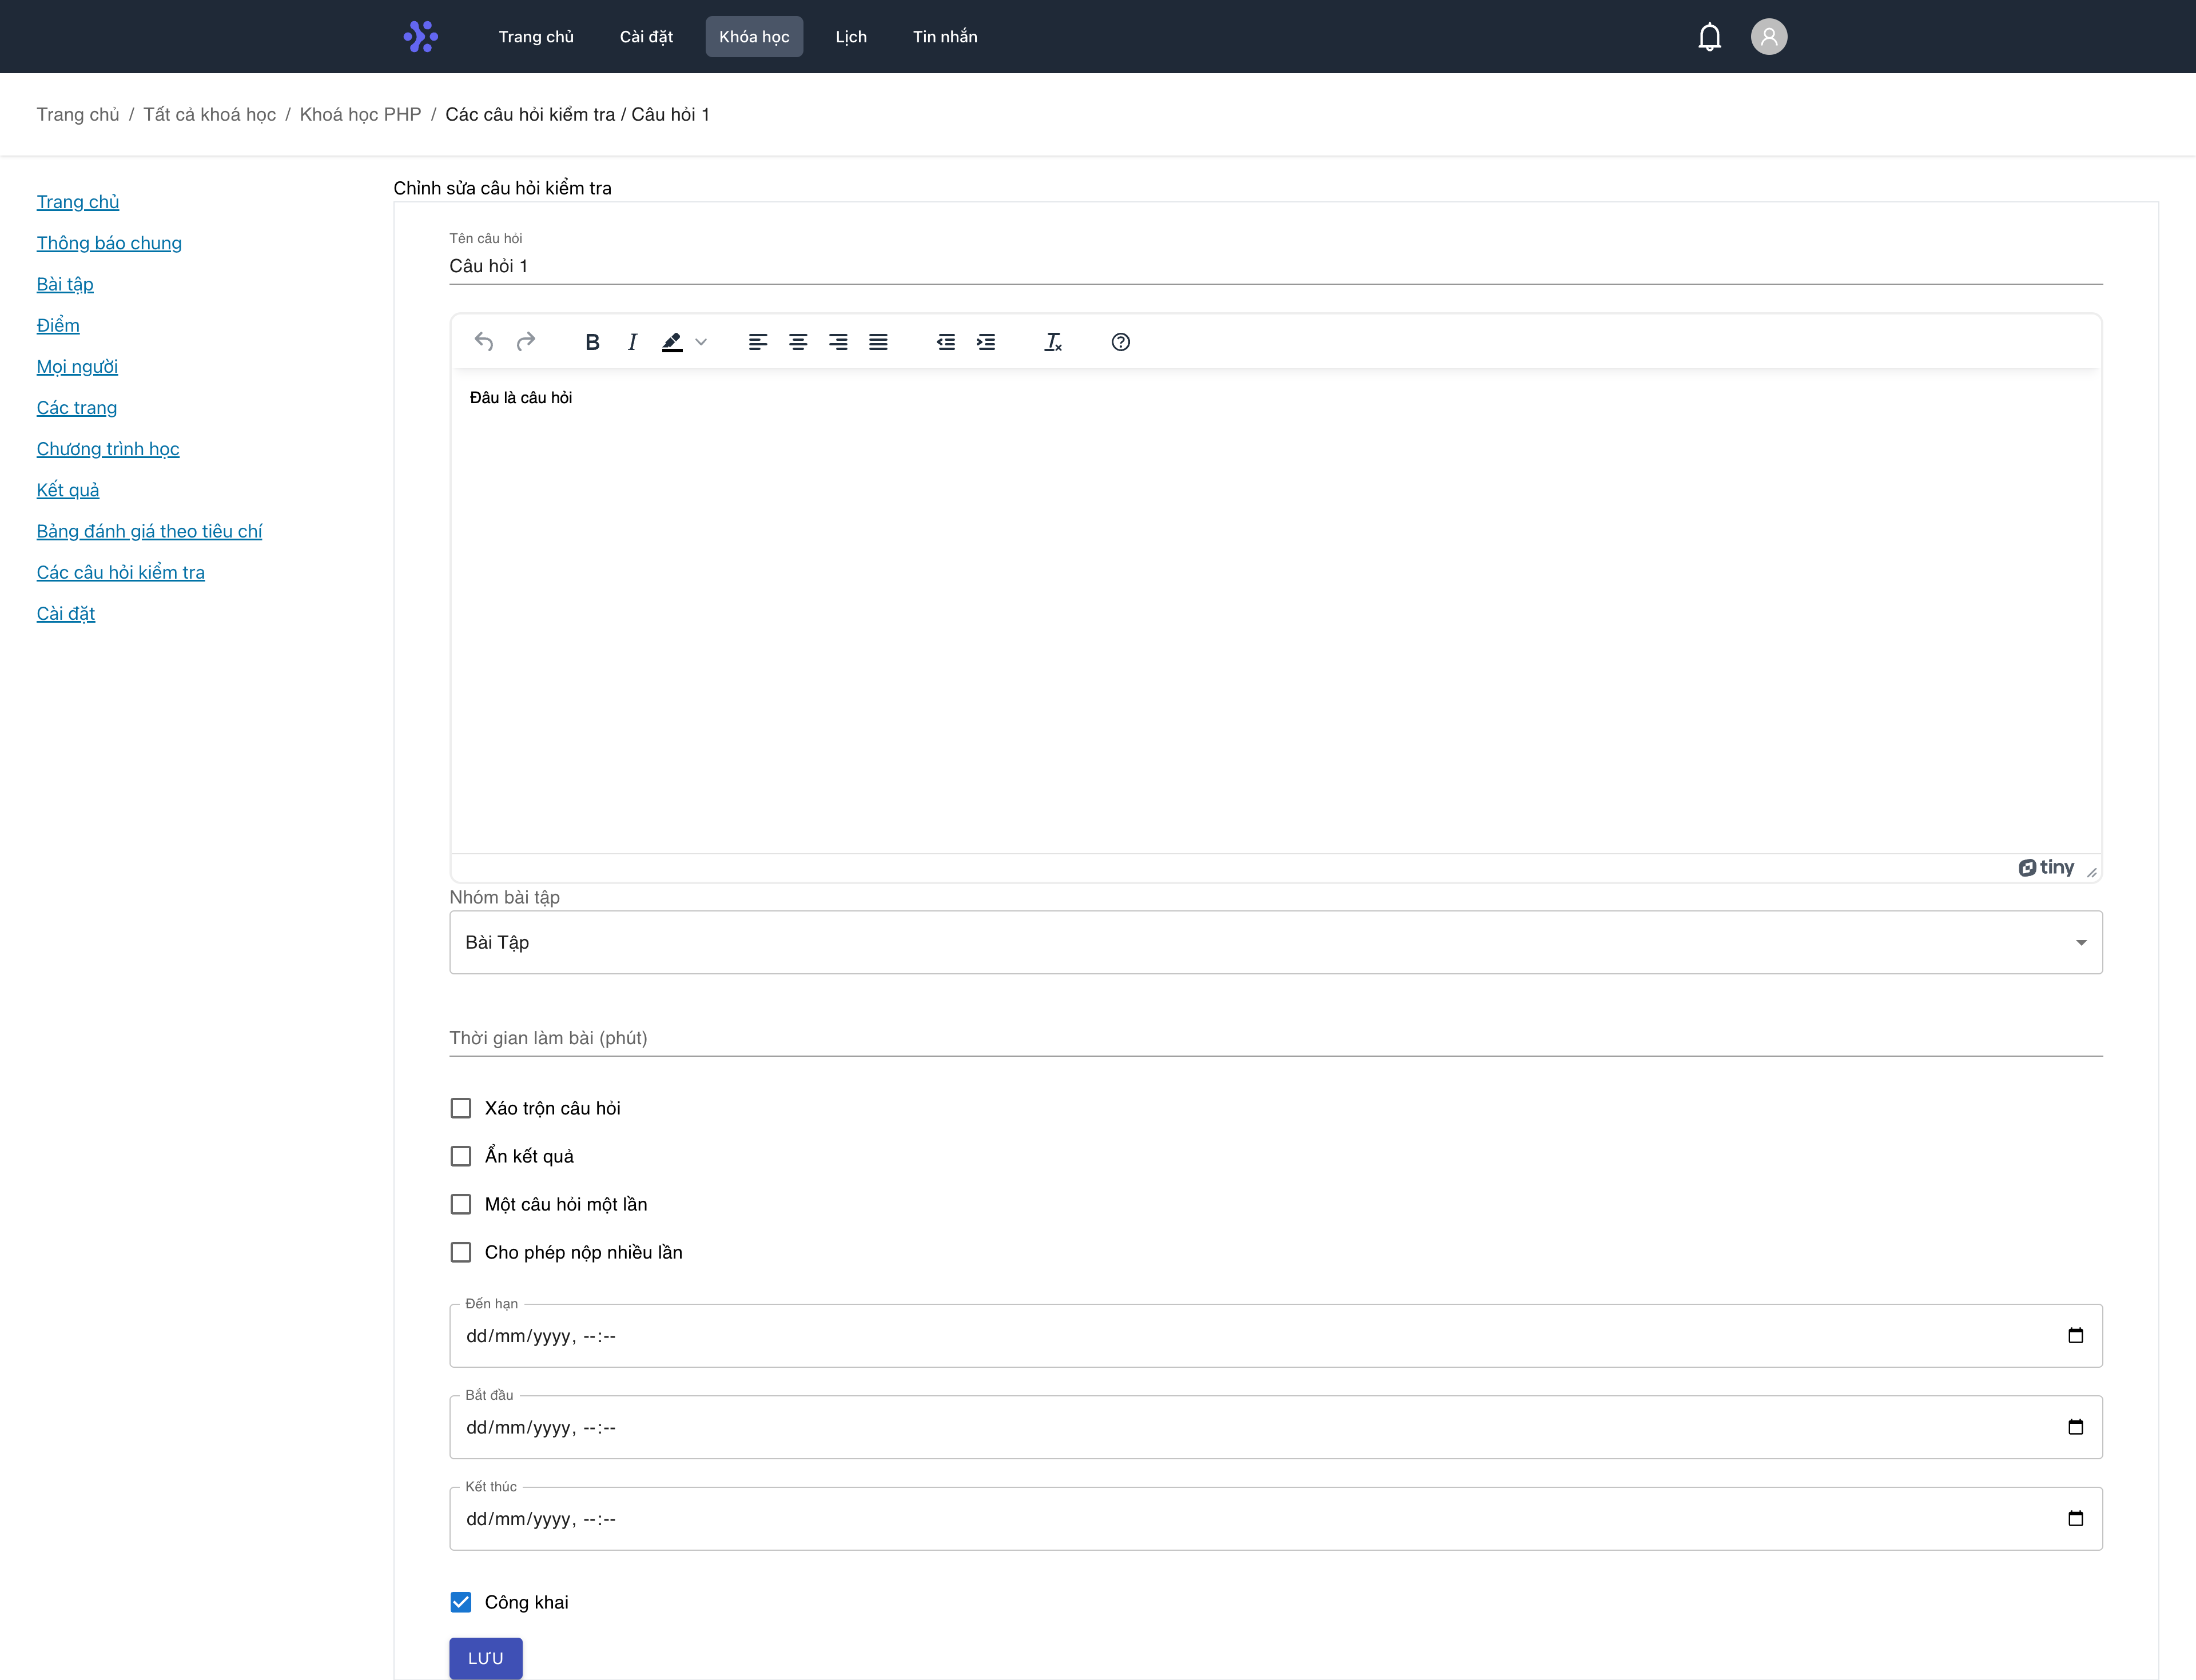
\includegraphics[width=300pt]{chinh-sua-cau-hoi-kiem-tra}
            \caption{Màn hình chỉnh sửa câu hỏi kiểm tra của phần quản trị viên}
            \label{fig:chinh-sua-cau-hoi-kiem-tra}
        \end{figure}

        Phần tạo câu hỏi trong câu hỏi kiểm tra của phần quản trị viên được thể hiện ở hình:
        \begin{figure}[ht!]
            \centering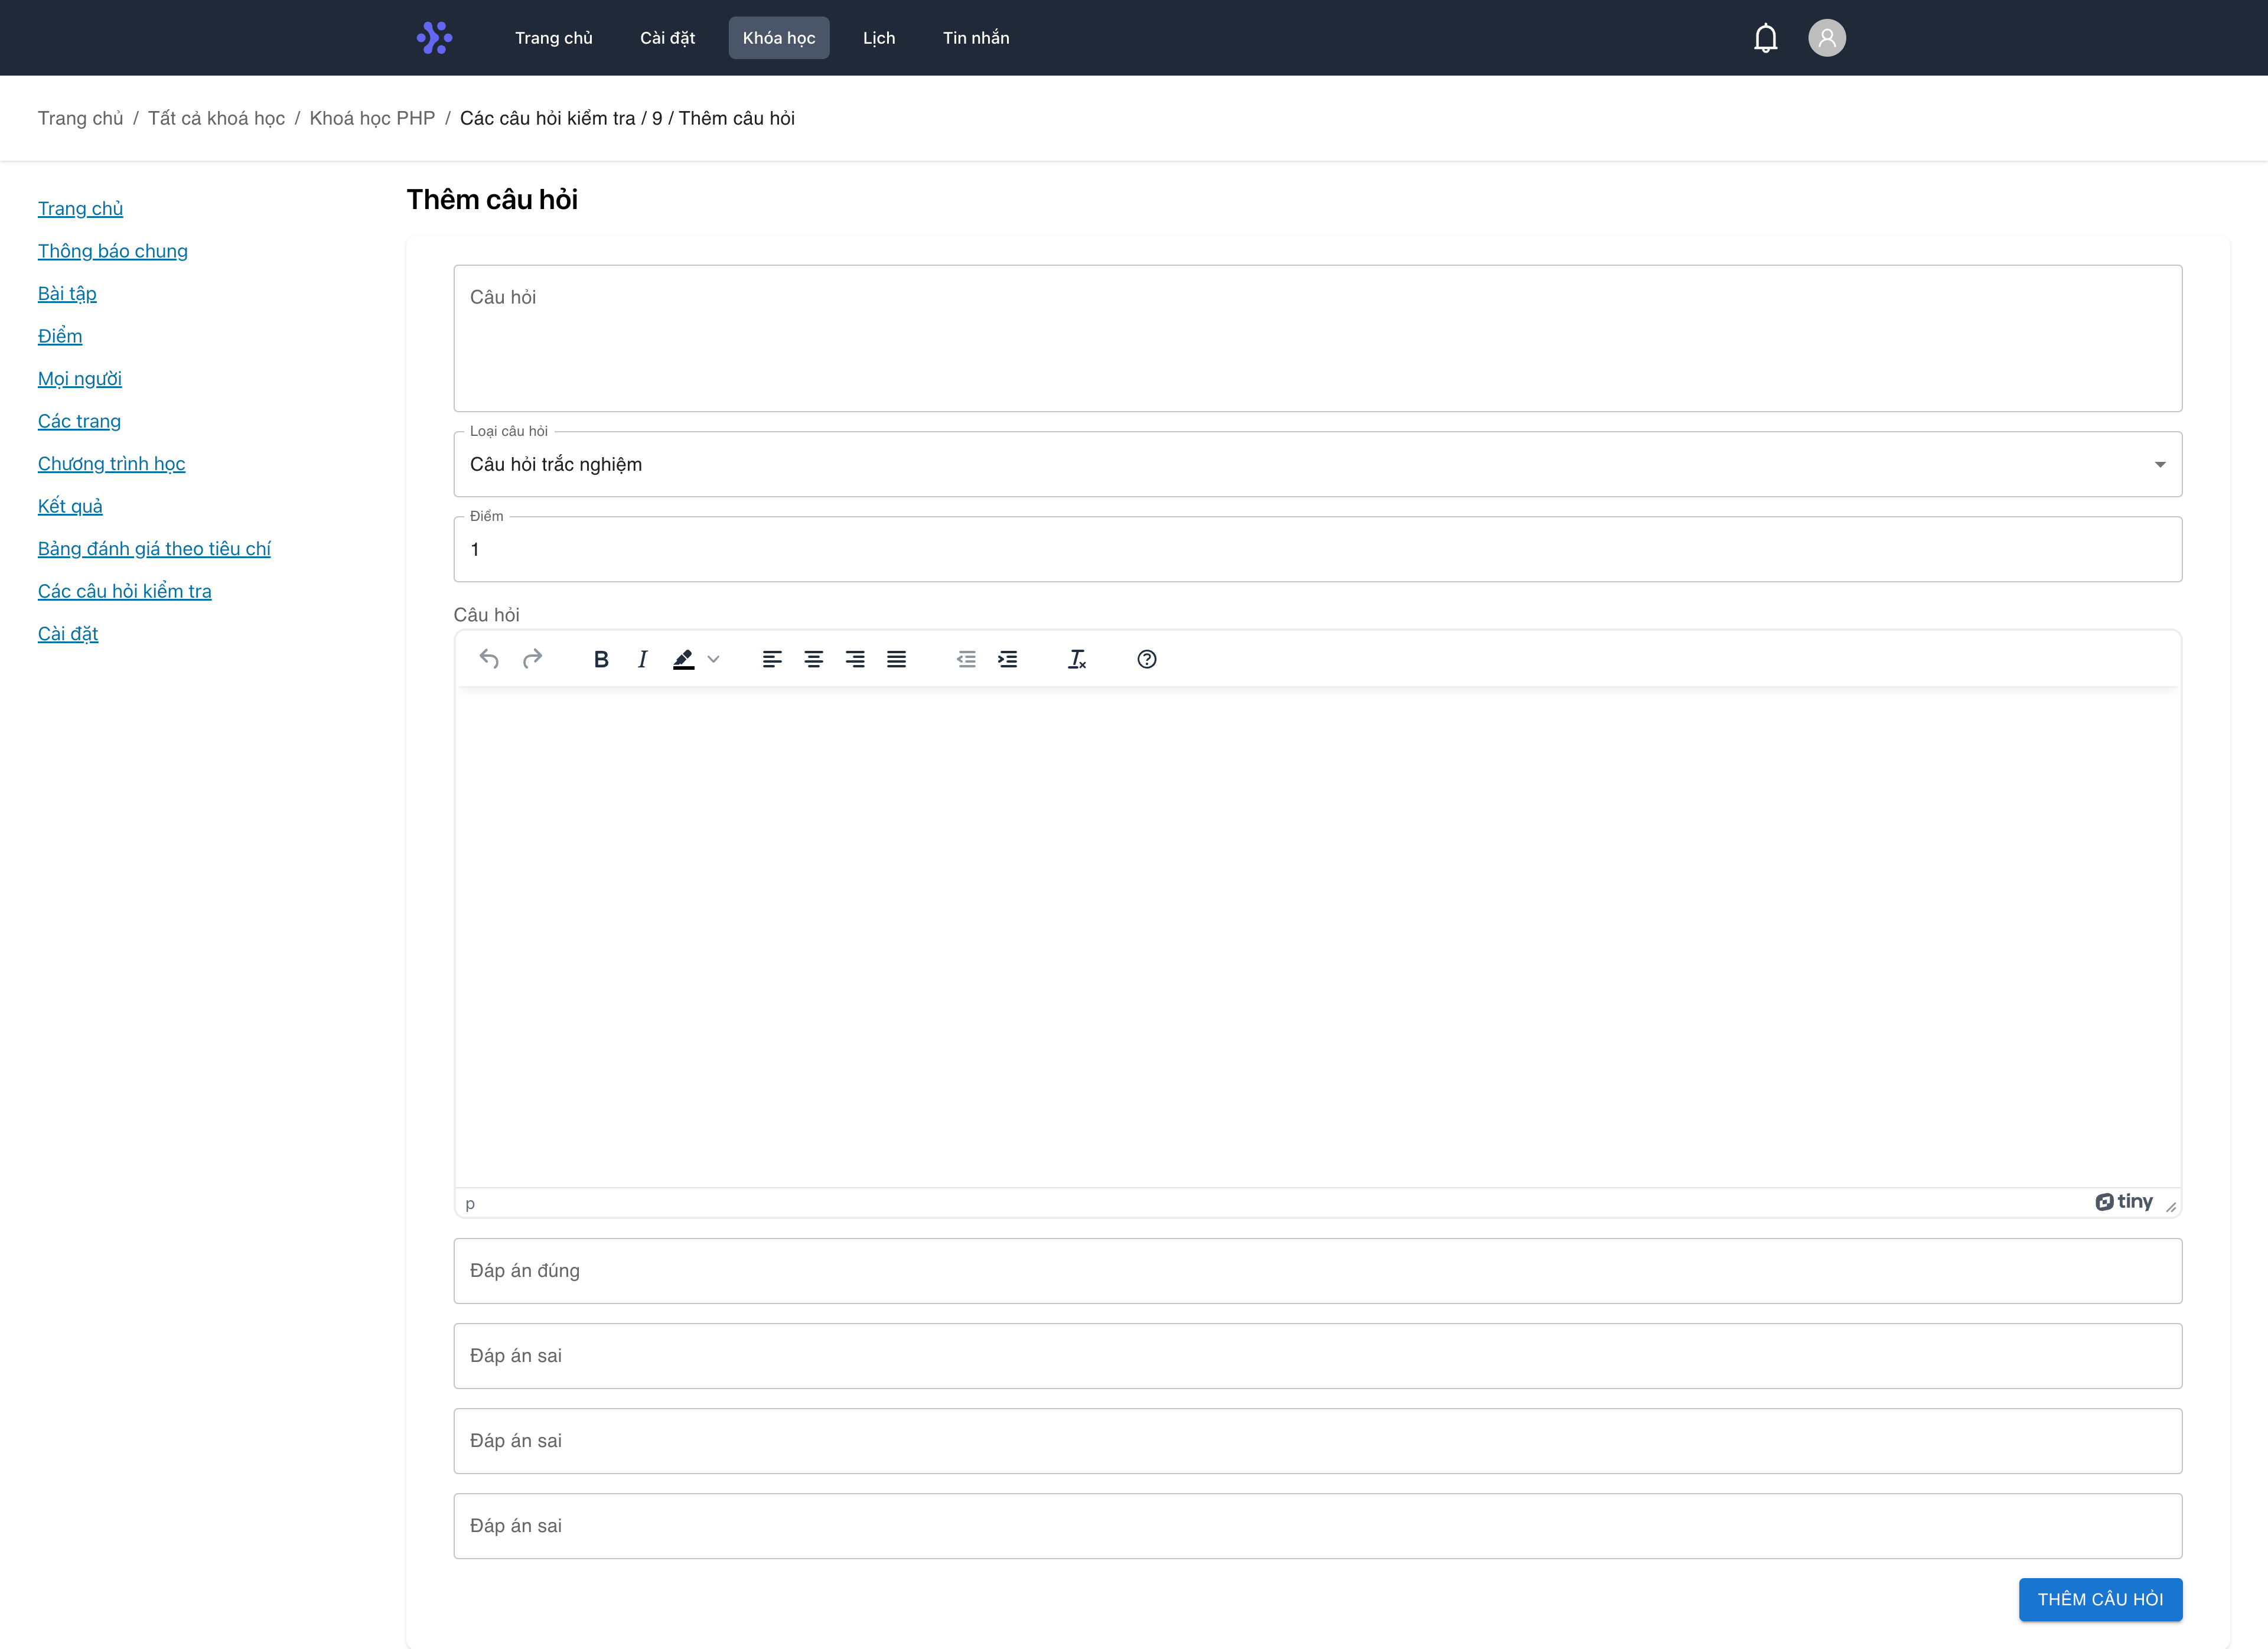
\includegraphics[width=300pt]{tao-cau-hoi-trong-cau-hoi-kiem-tra}
            \caption{Màn hình tạo câu hỏi trong câu hỏi kiểm tra của phần quản trị viên}
            \label{fig:tao-cau-hoi-trong-cau-hoi-kiem-tra}
        \end{figure}

        Phần chỉnh sửa câu hỏi trong câu hỏi kiểm tra của phần quản trị viên được thể hiện ở hình:
        \begin{figure}[ht!]
            \centering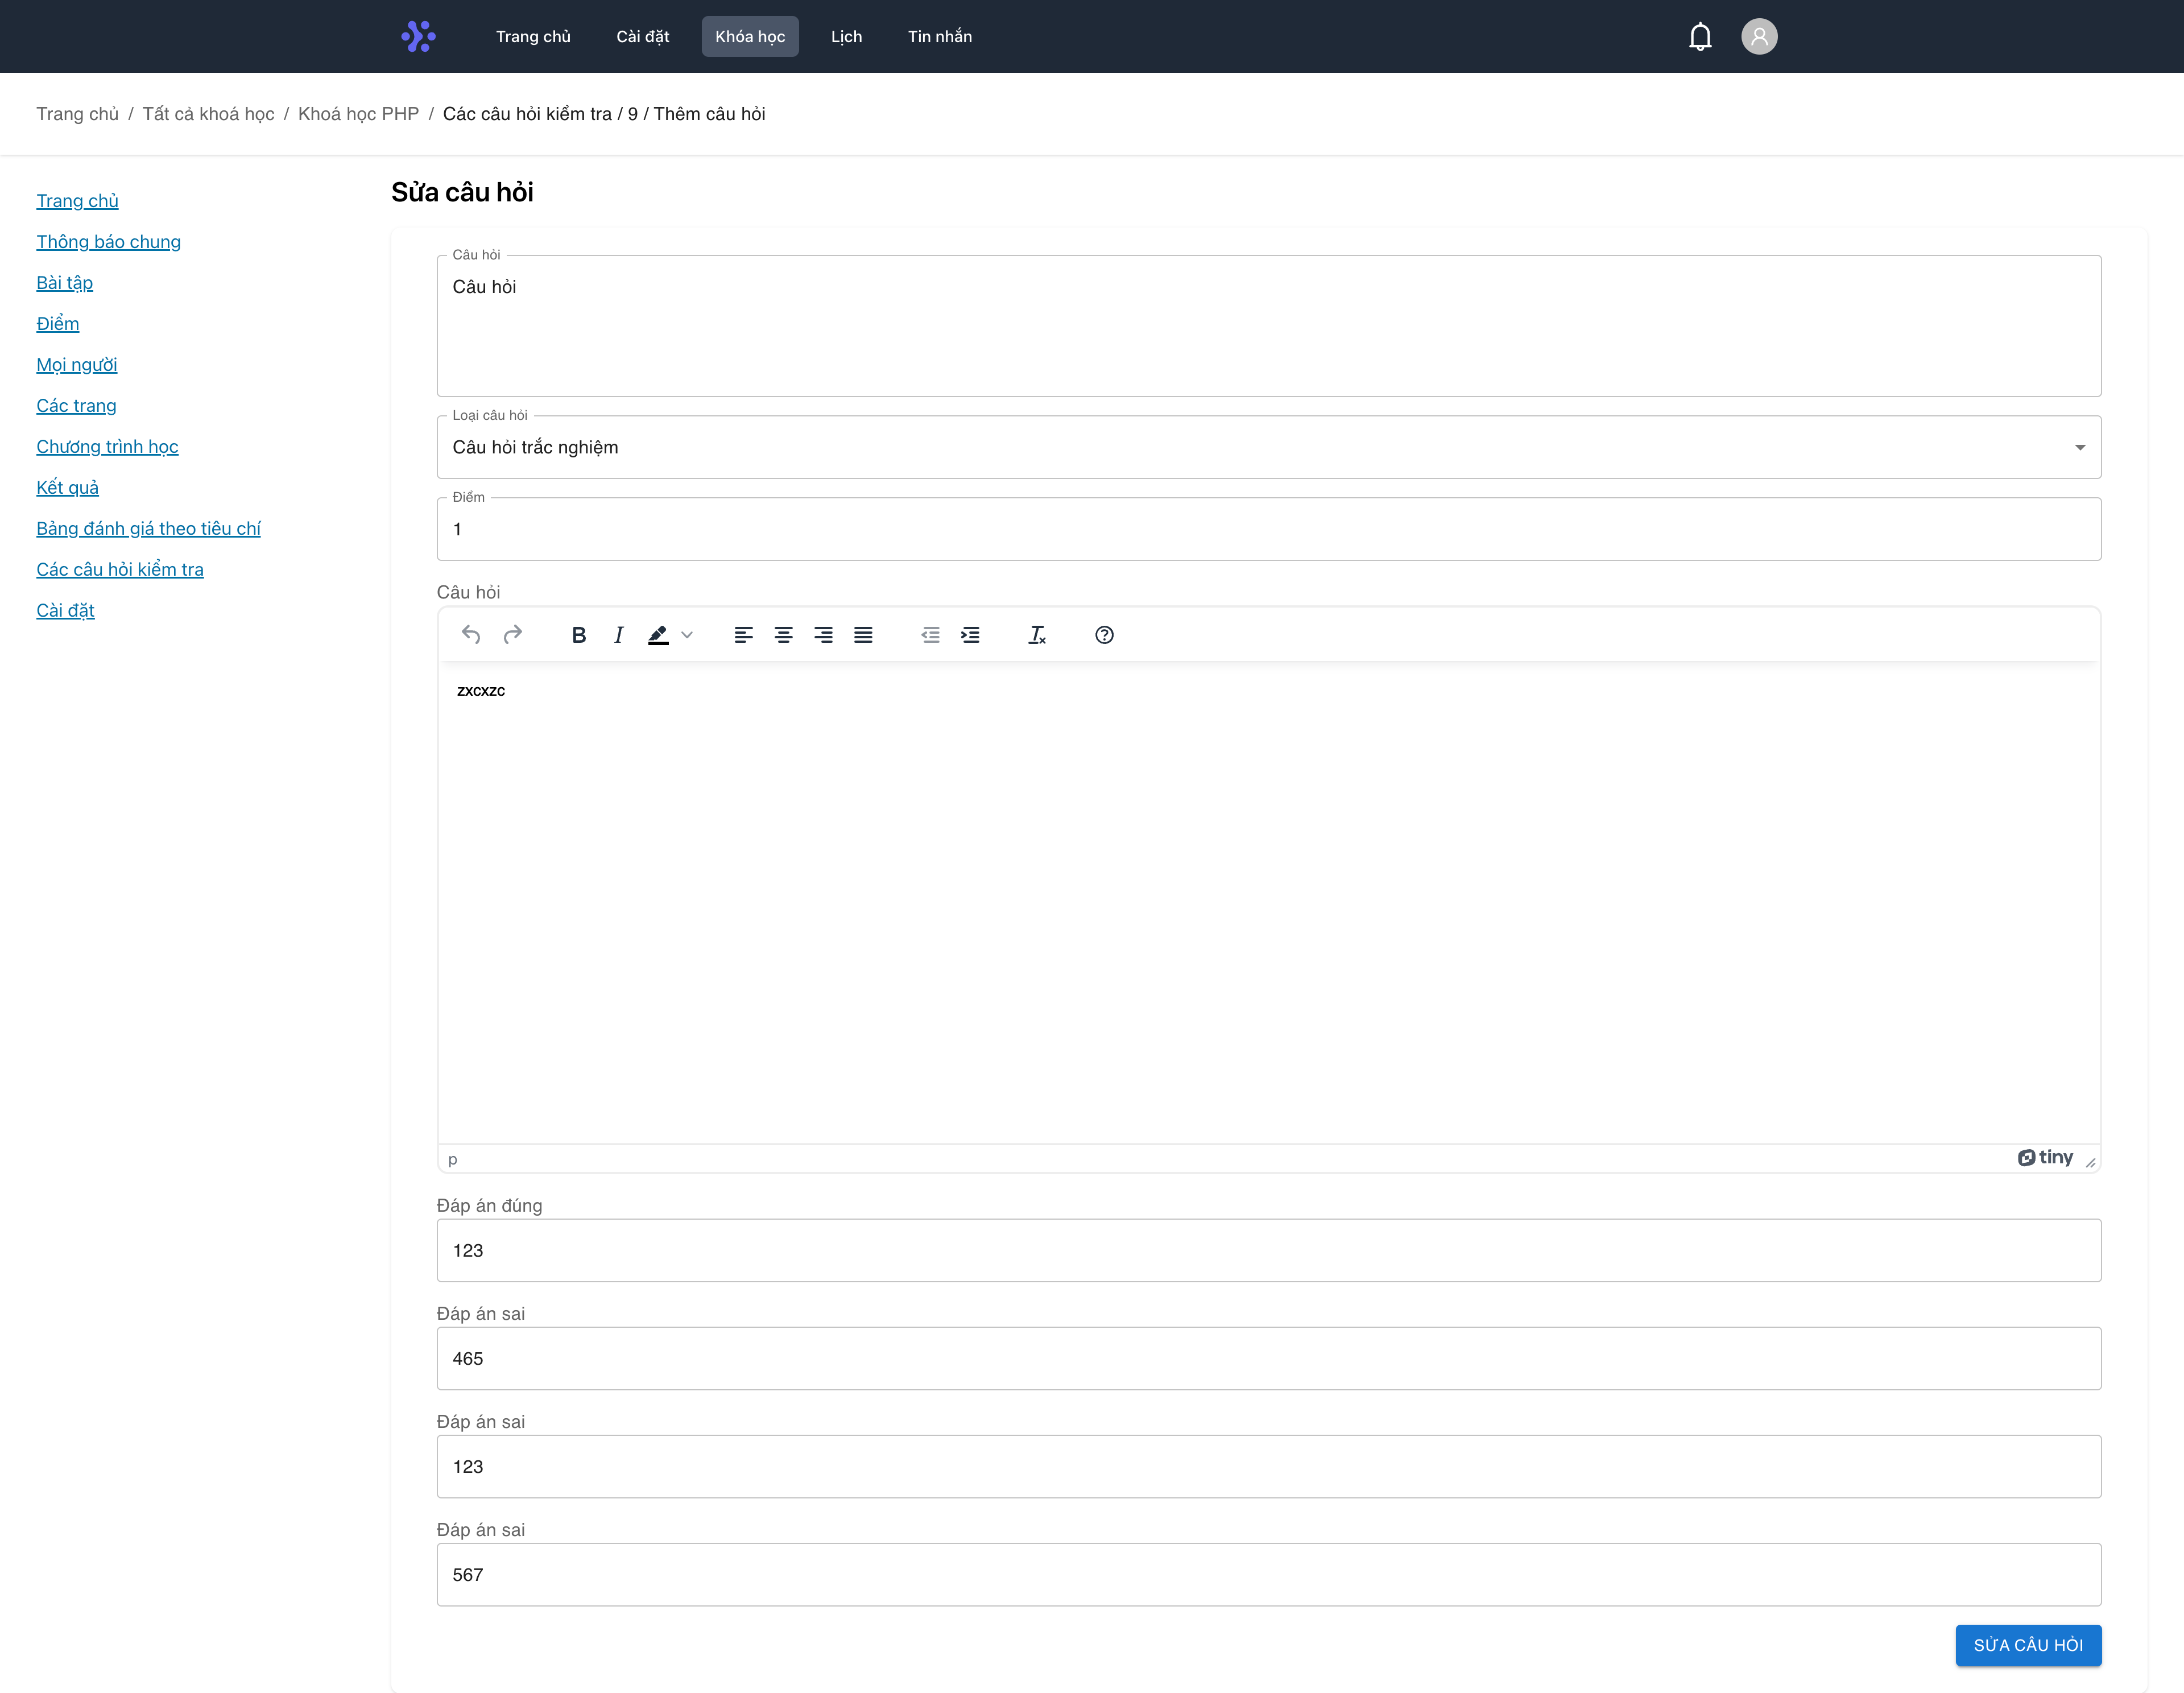
\includegraphics[width=300pt]{chinh-sua-cau-hoi-trong-cau-hoi-kiem-tra}
            \caption{Màn hình chỉnh sửa câu hỏi trong câu hỏi kiểm tra của phần quản trị viên}
            \label{fig:chinh-sua-cau-hoi-trong-cau-hoi-kiem-tra}
        \end{figure}

        Phần lịch sử của phần quản trị viên được thể hiện ở hình:
        \begin{figure}[ht!]
            \centering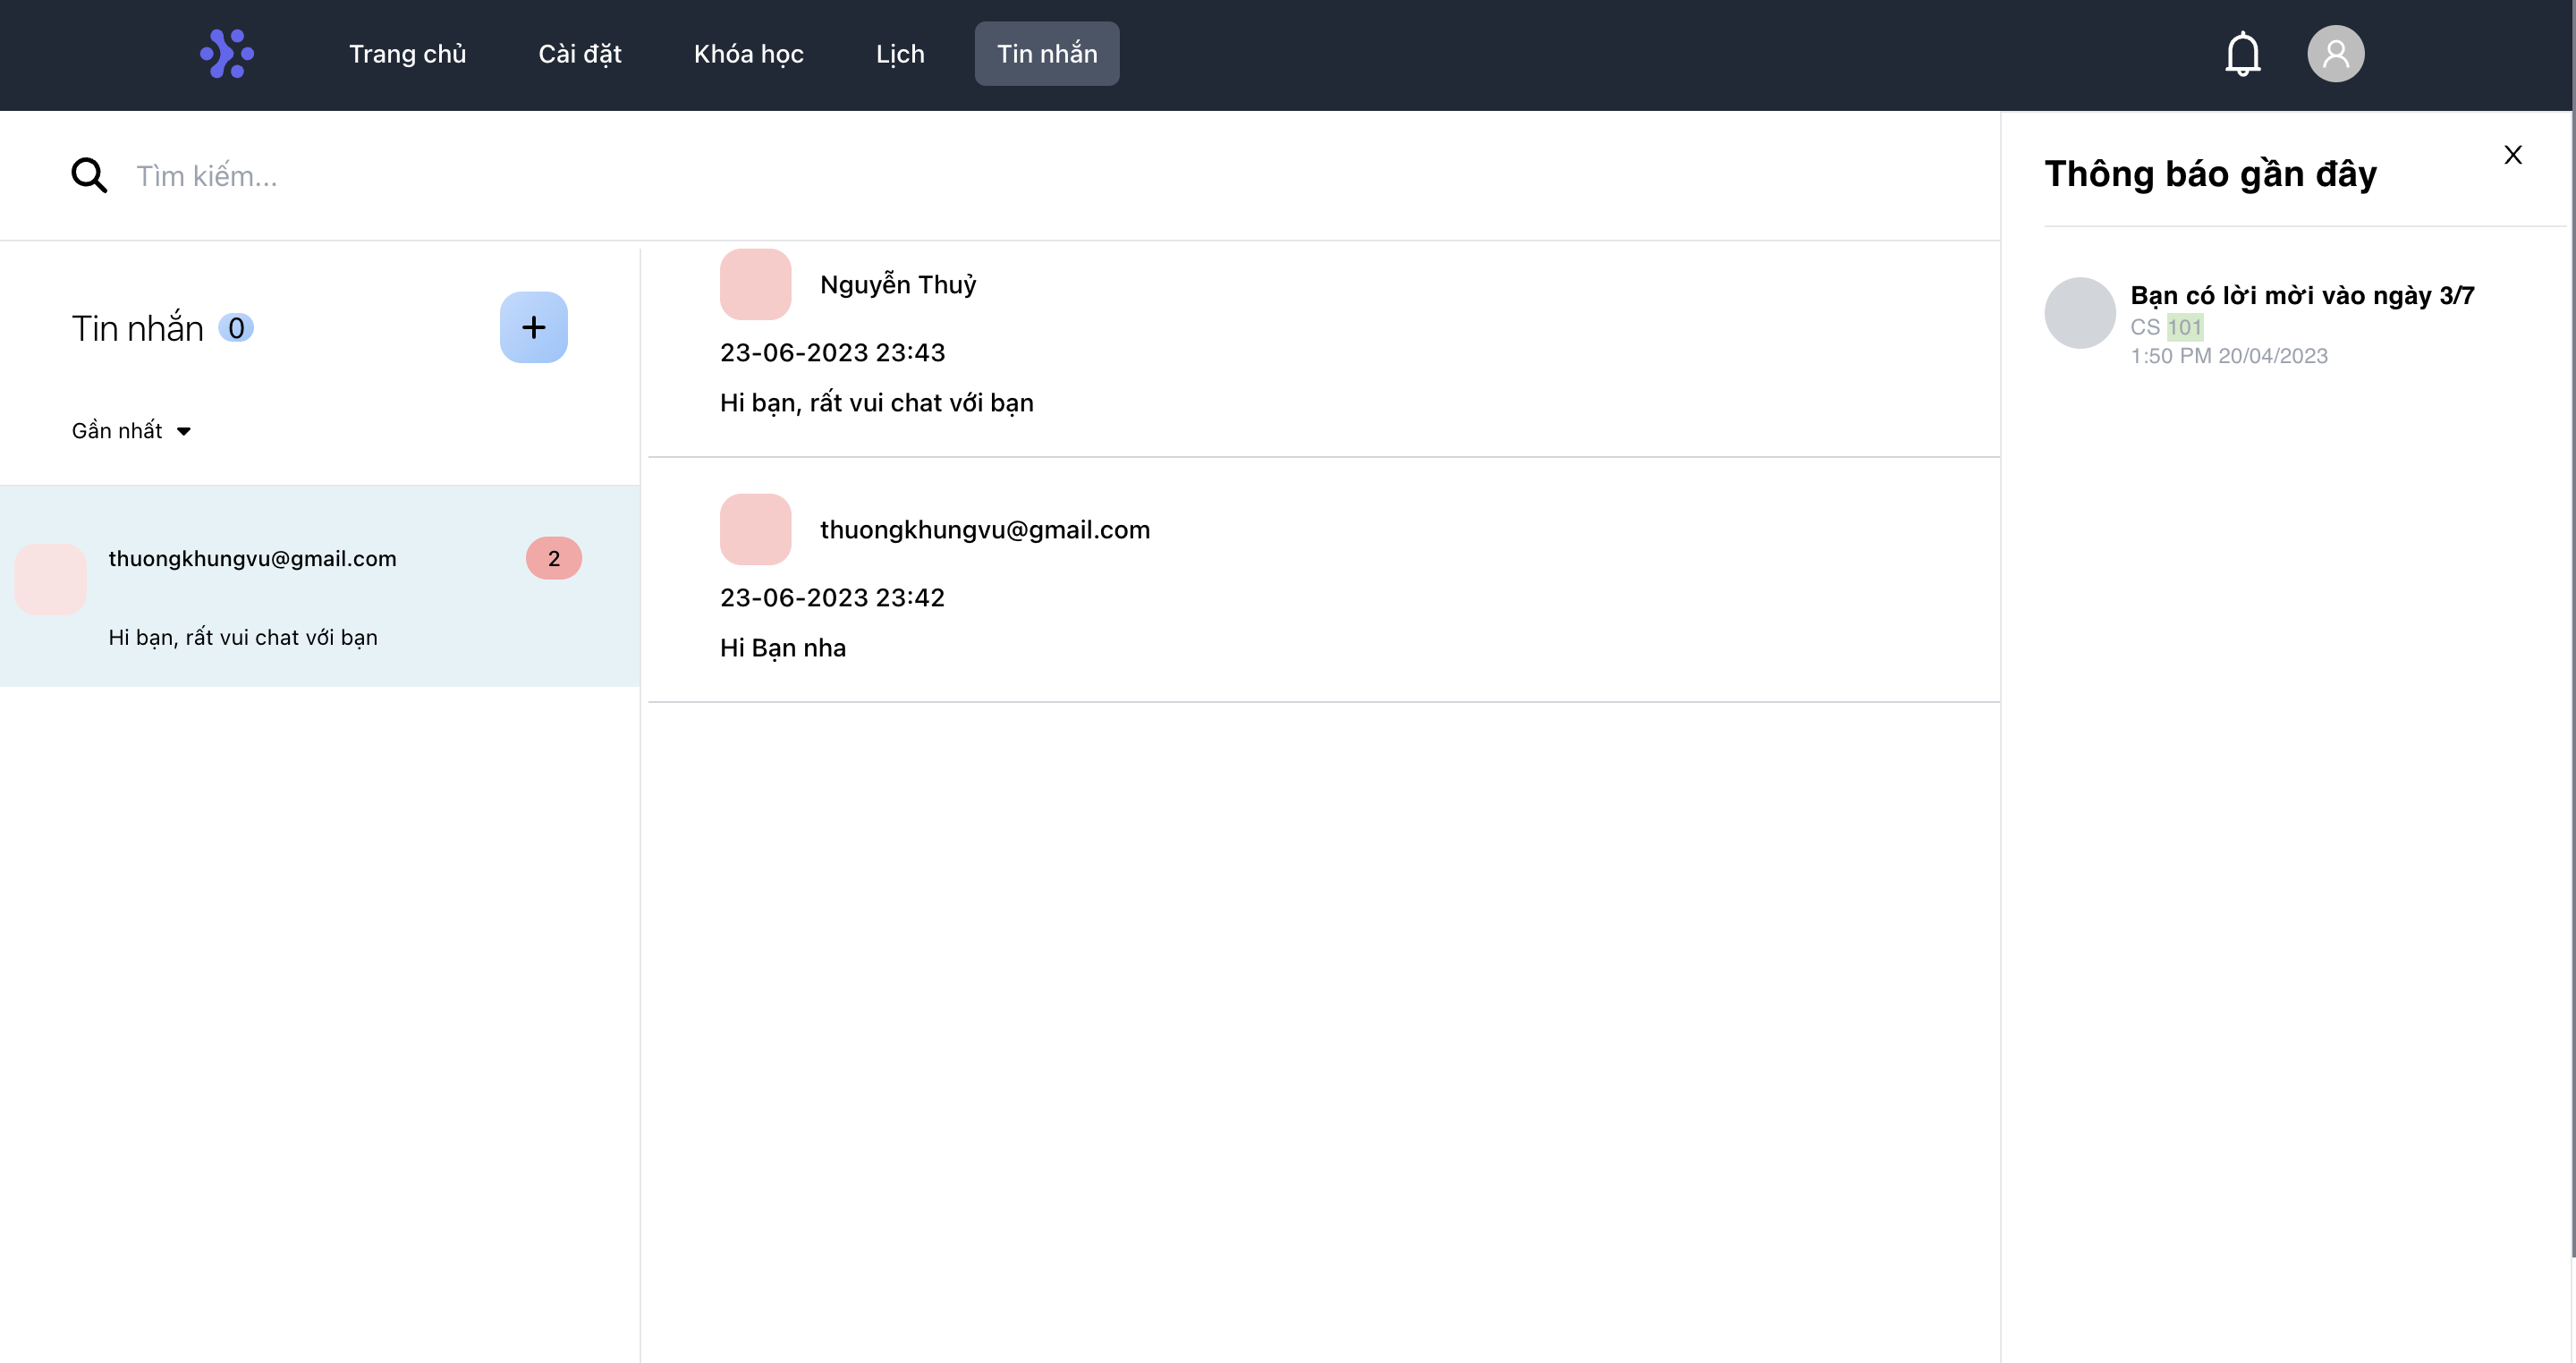
\includegraphics[width=300pt]{lich-su}
            \caption{Màn hình lịch sử của phần quản trị viên}
            \label{fig:lich-su}
        \end{figure}

        Phần sự kiện của phần quản trị viên được thể hiện ở hình:
        \begin{figure}[ht!]
            \centering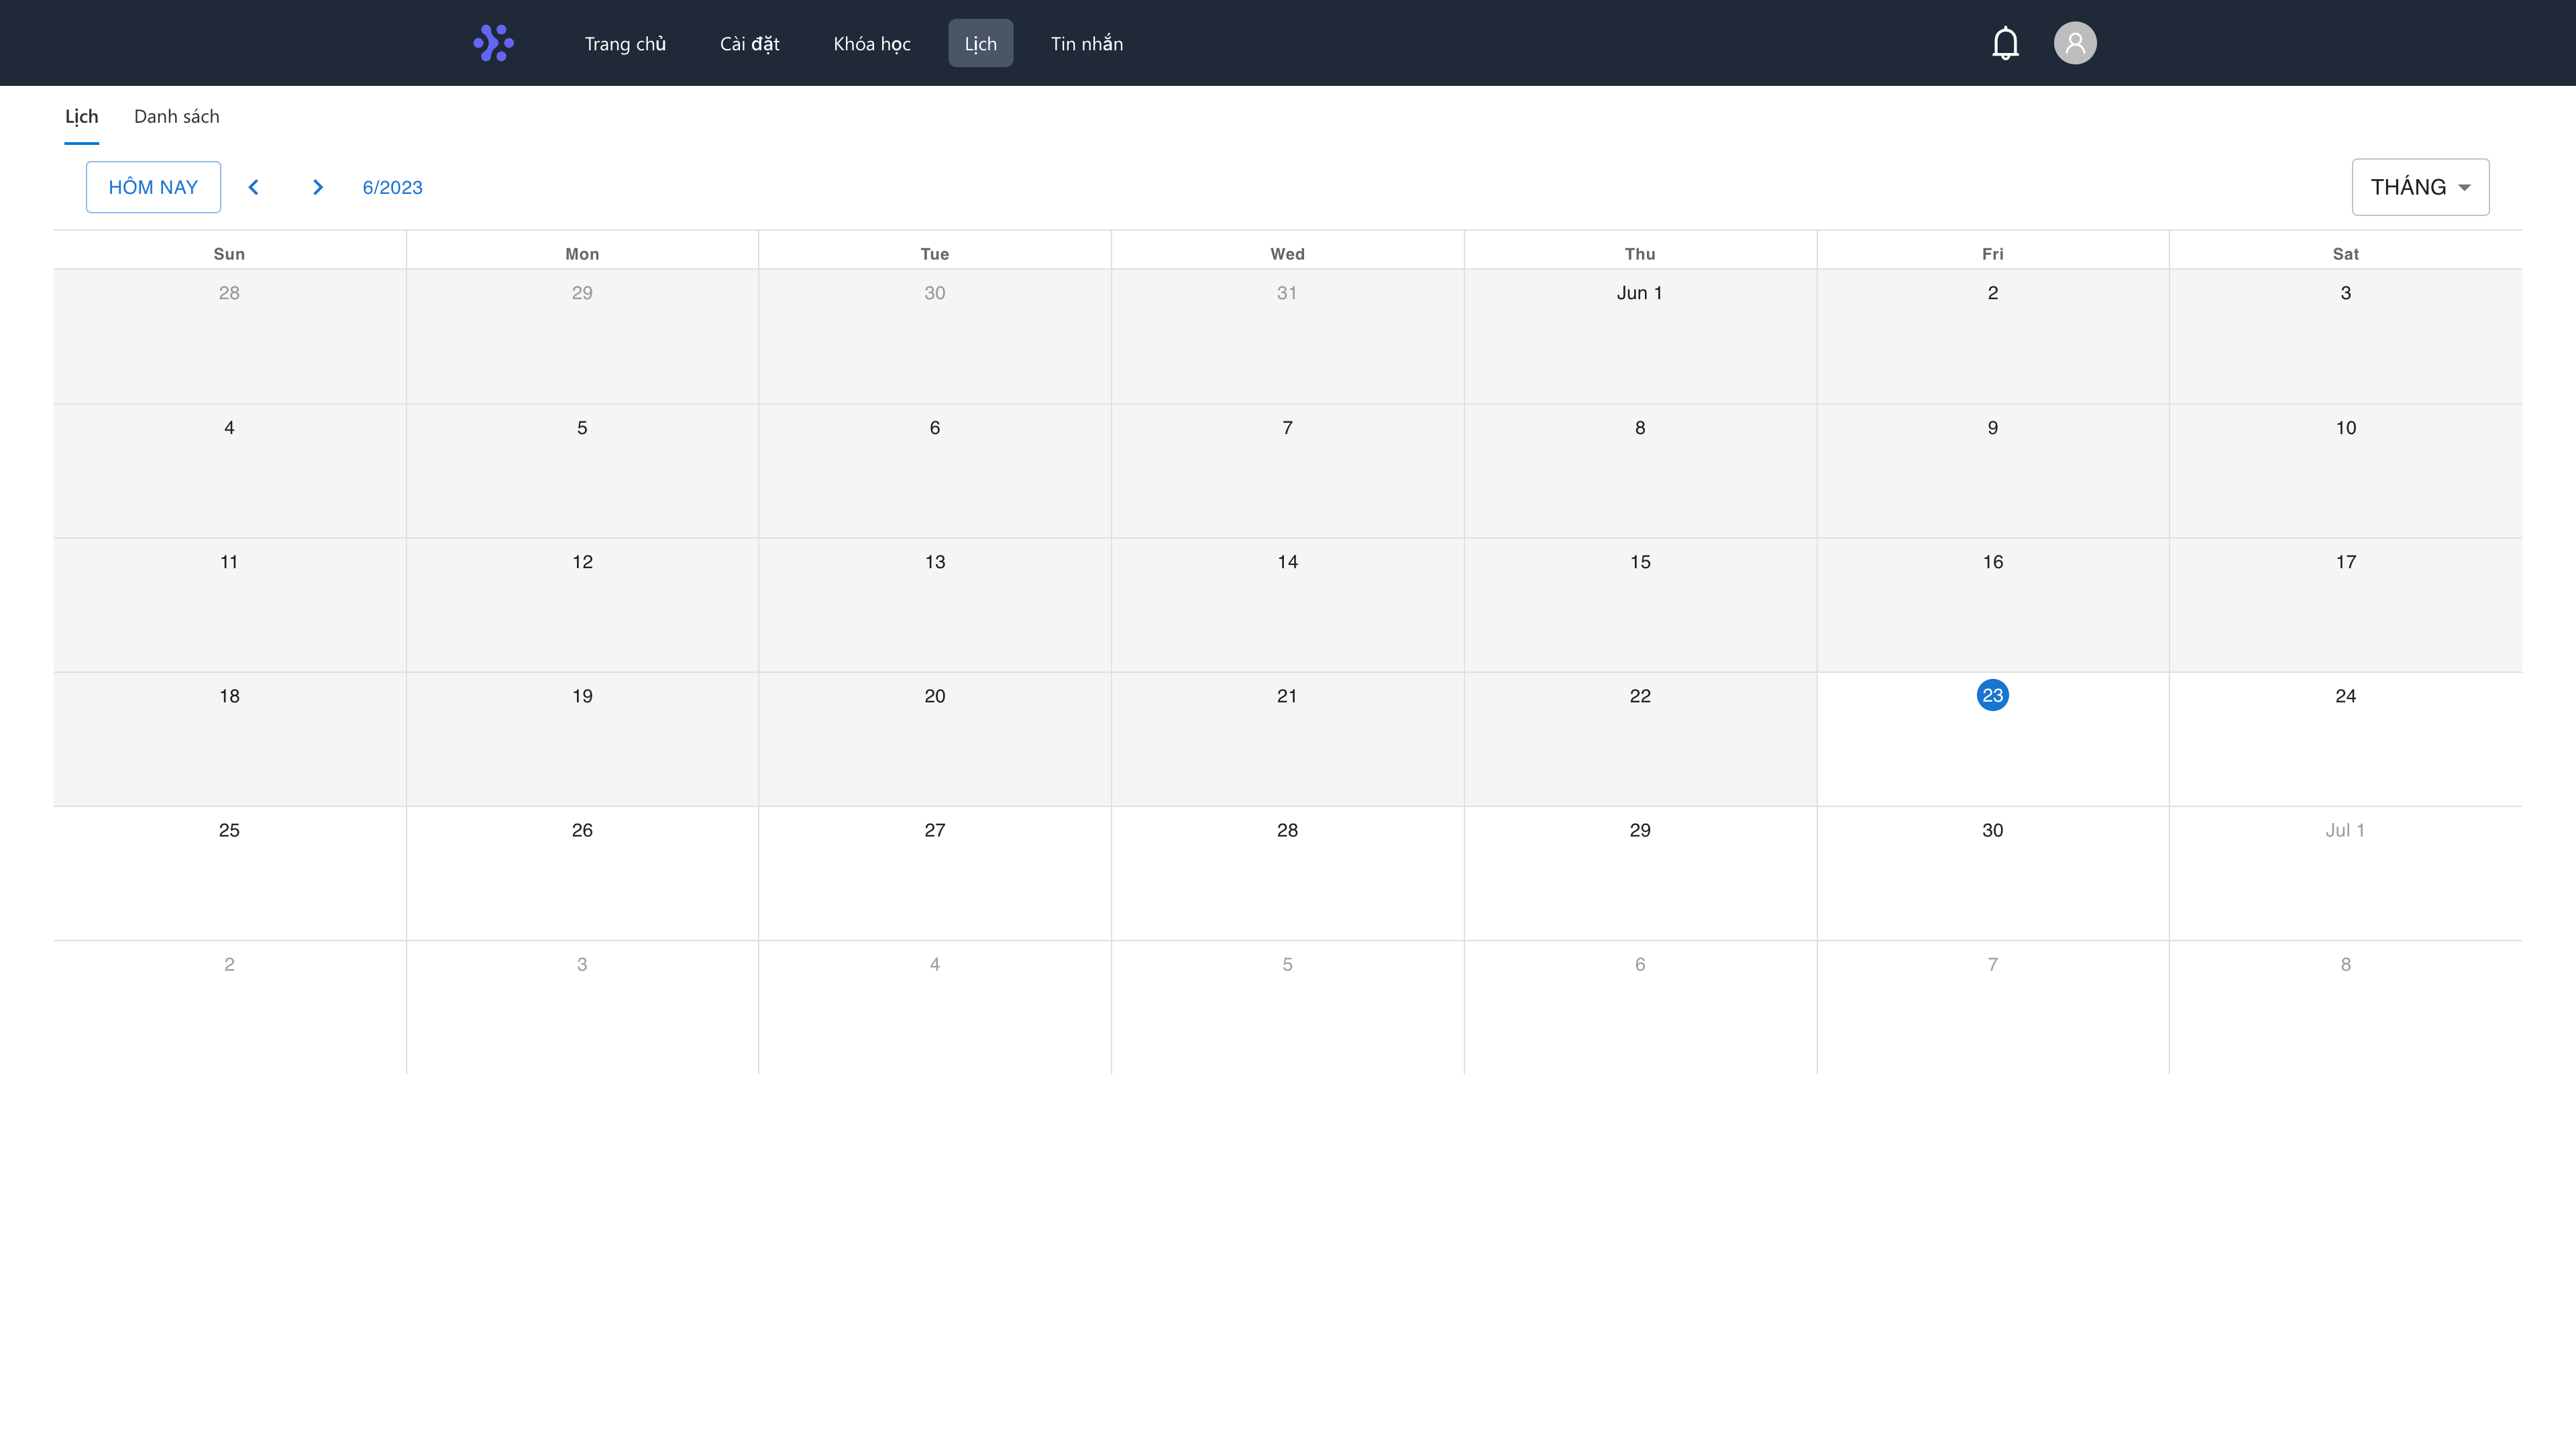
\includegraphics[width=300pt]{su-kien}
            \caption{Màn hình sự kiện của phần quản trị viên}
            \label{fig:su-kien}
        \end{figure}

        Phần danh sách sự kiện của phần quản trị viên được thể hiện ở hình:
        \begin{figure}[ht!]
            \centering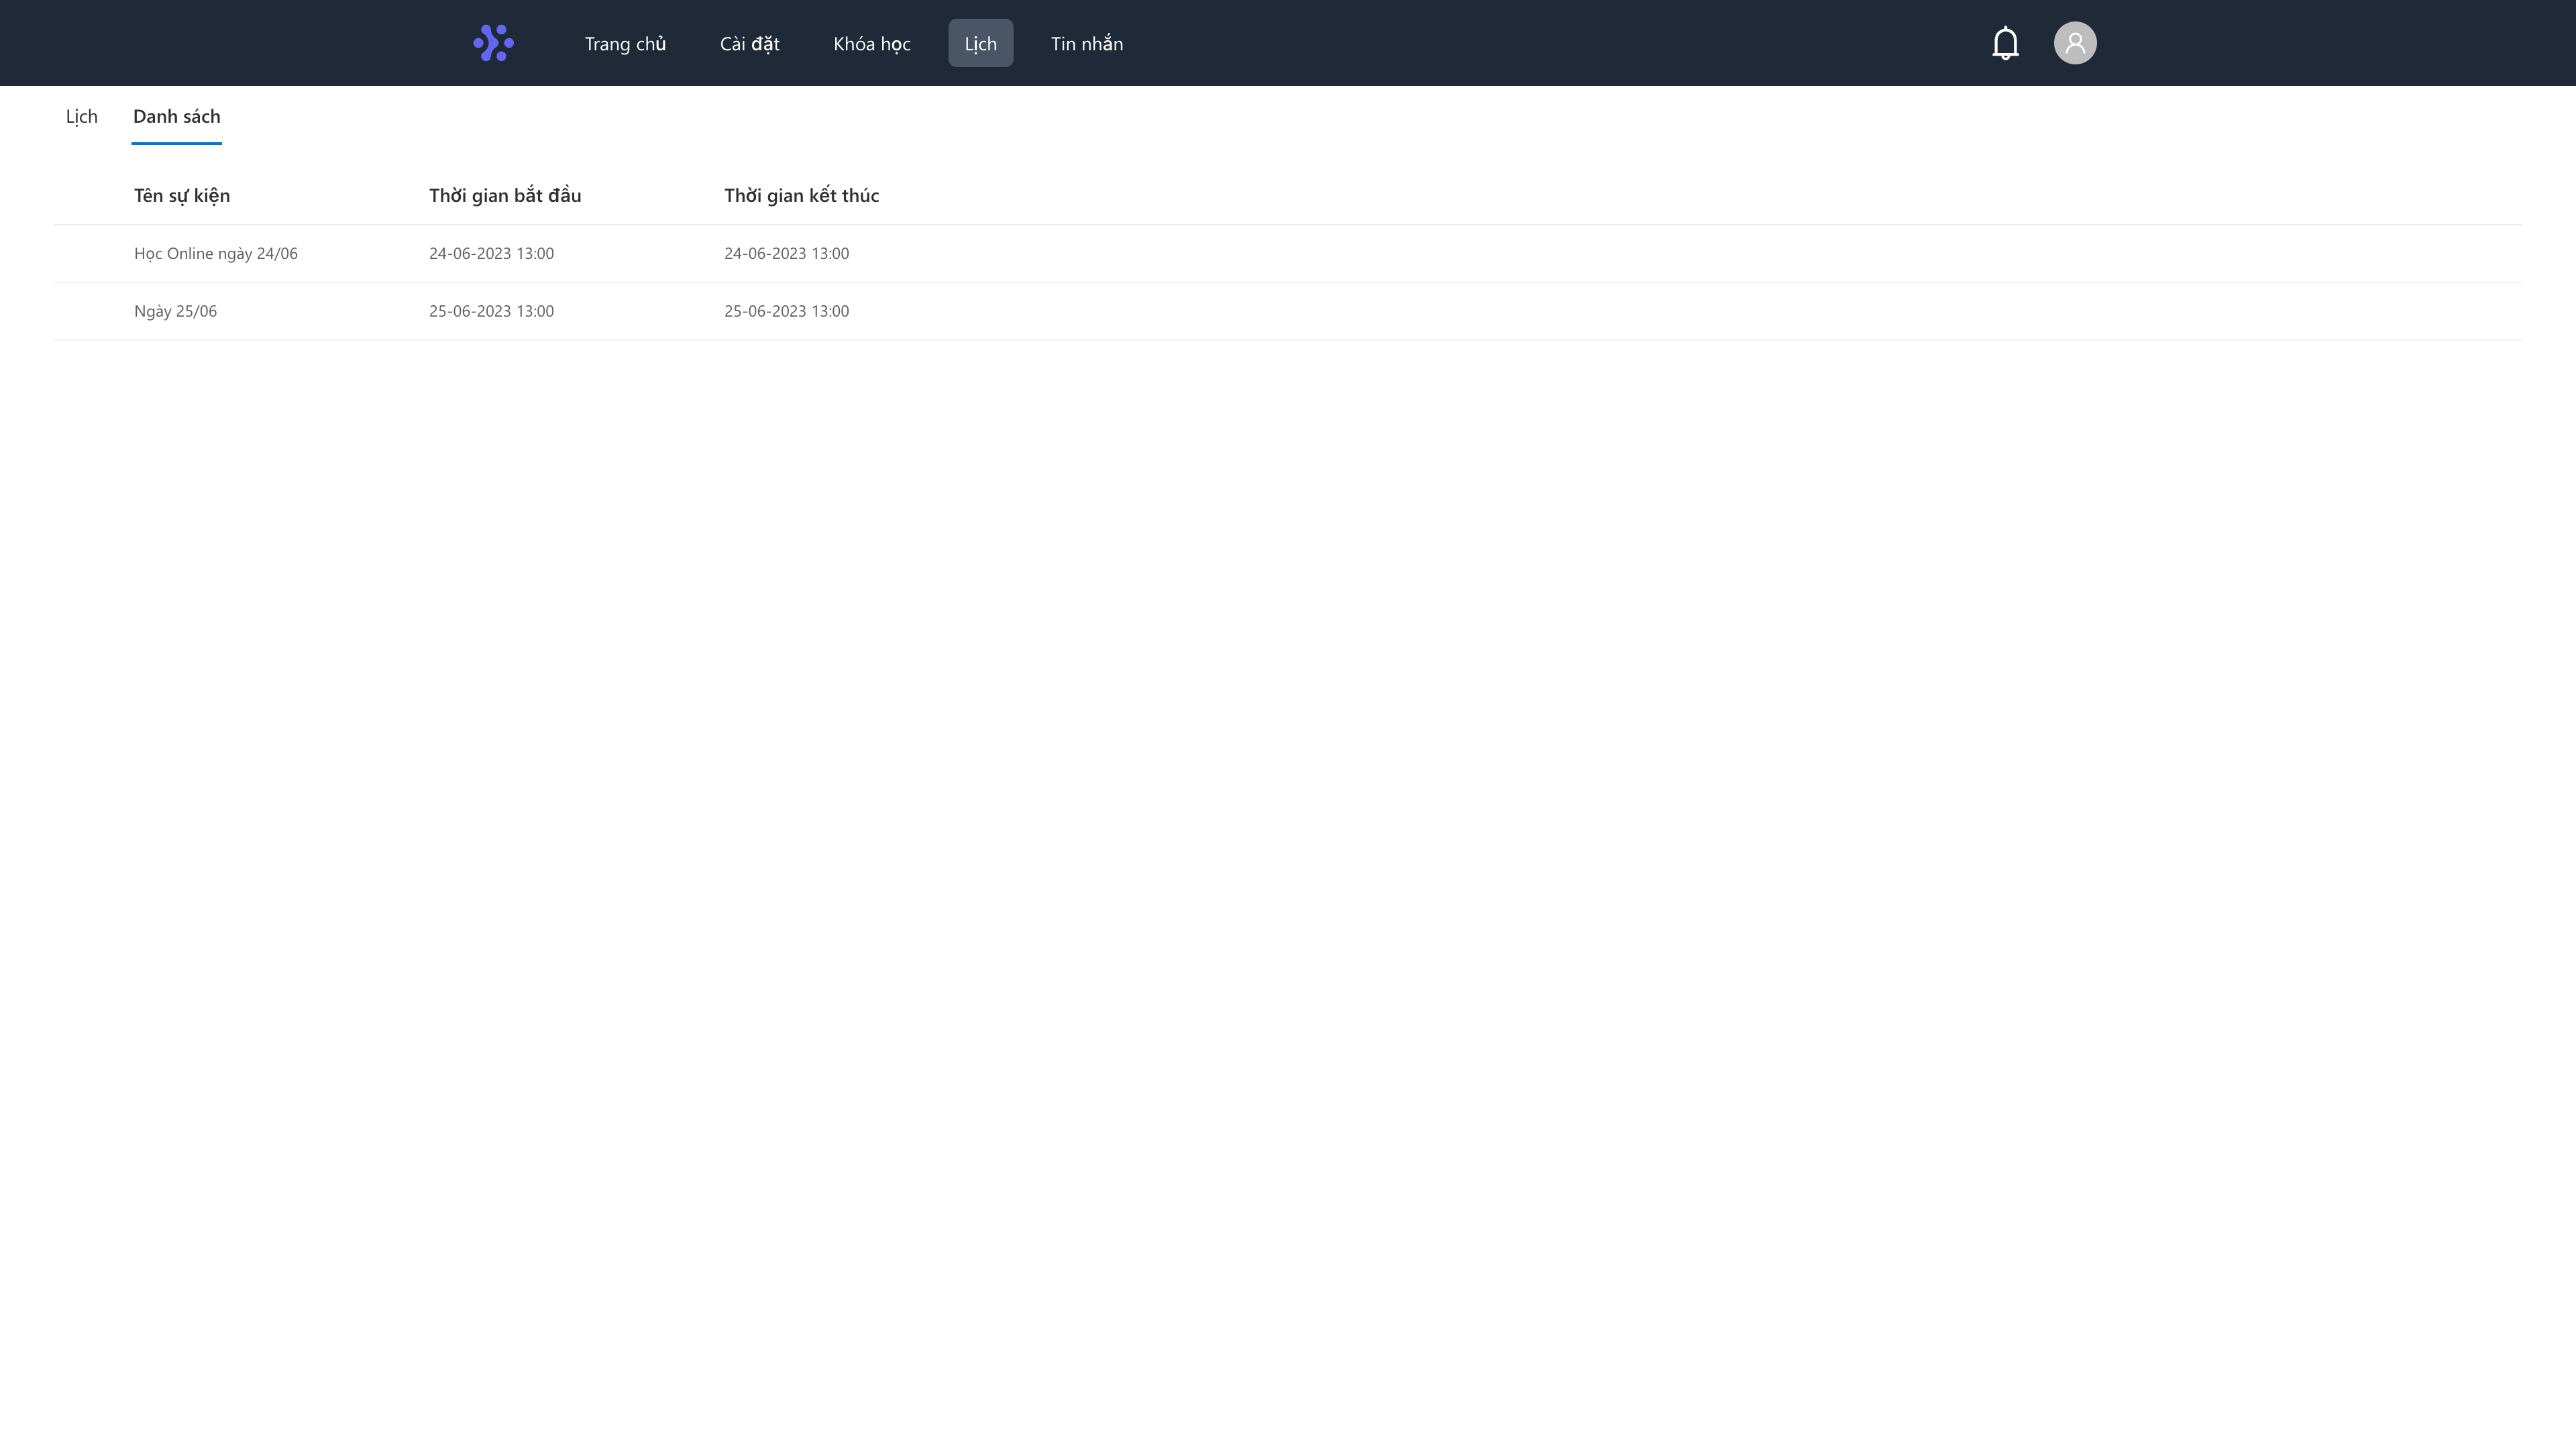
\includegraphics[width=300pt]{danh-sach-su-kien}
            \caption{Màn hình danh sách sự kiện của phần quản trị viên}
            \label{fig:danh-sach-su-kien}
        \end{figure}

        Phần tạo sự kiện của phần quản trị viên được thể hiện ở hình:
        \begin{figure}[ht!]
            \centering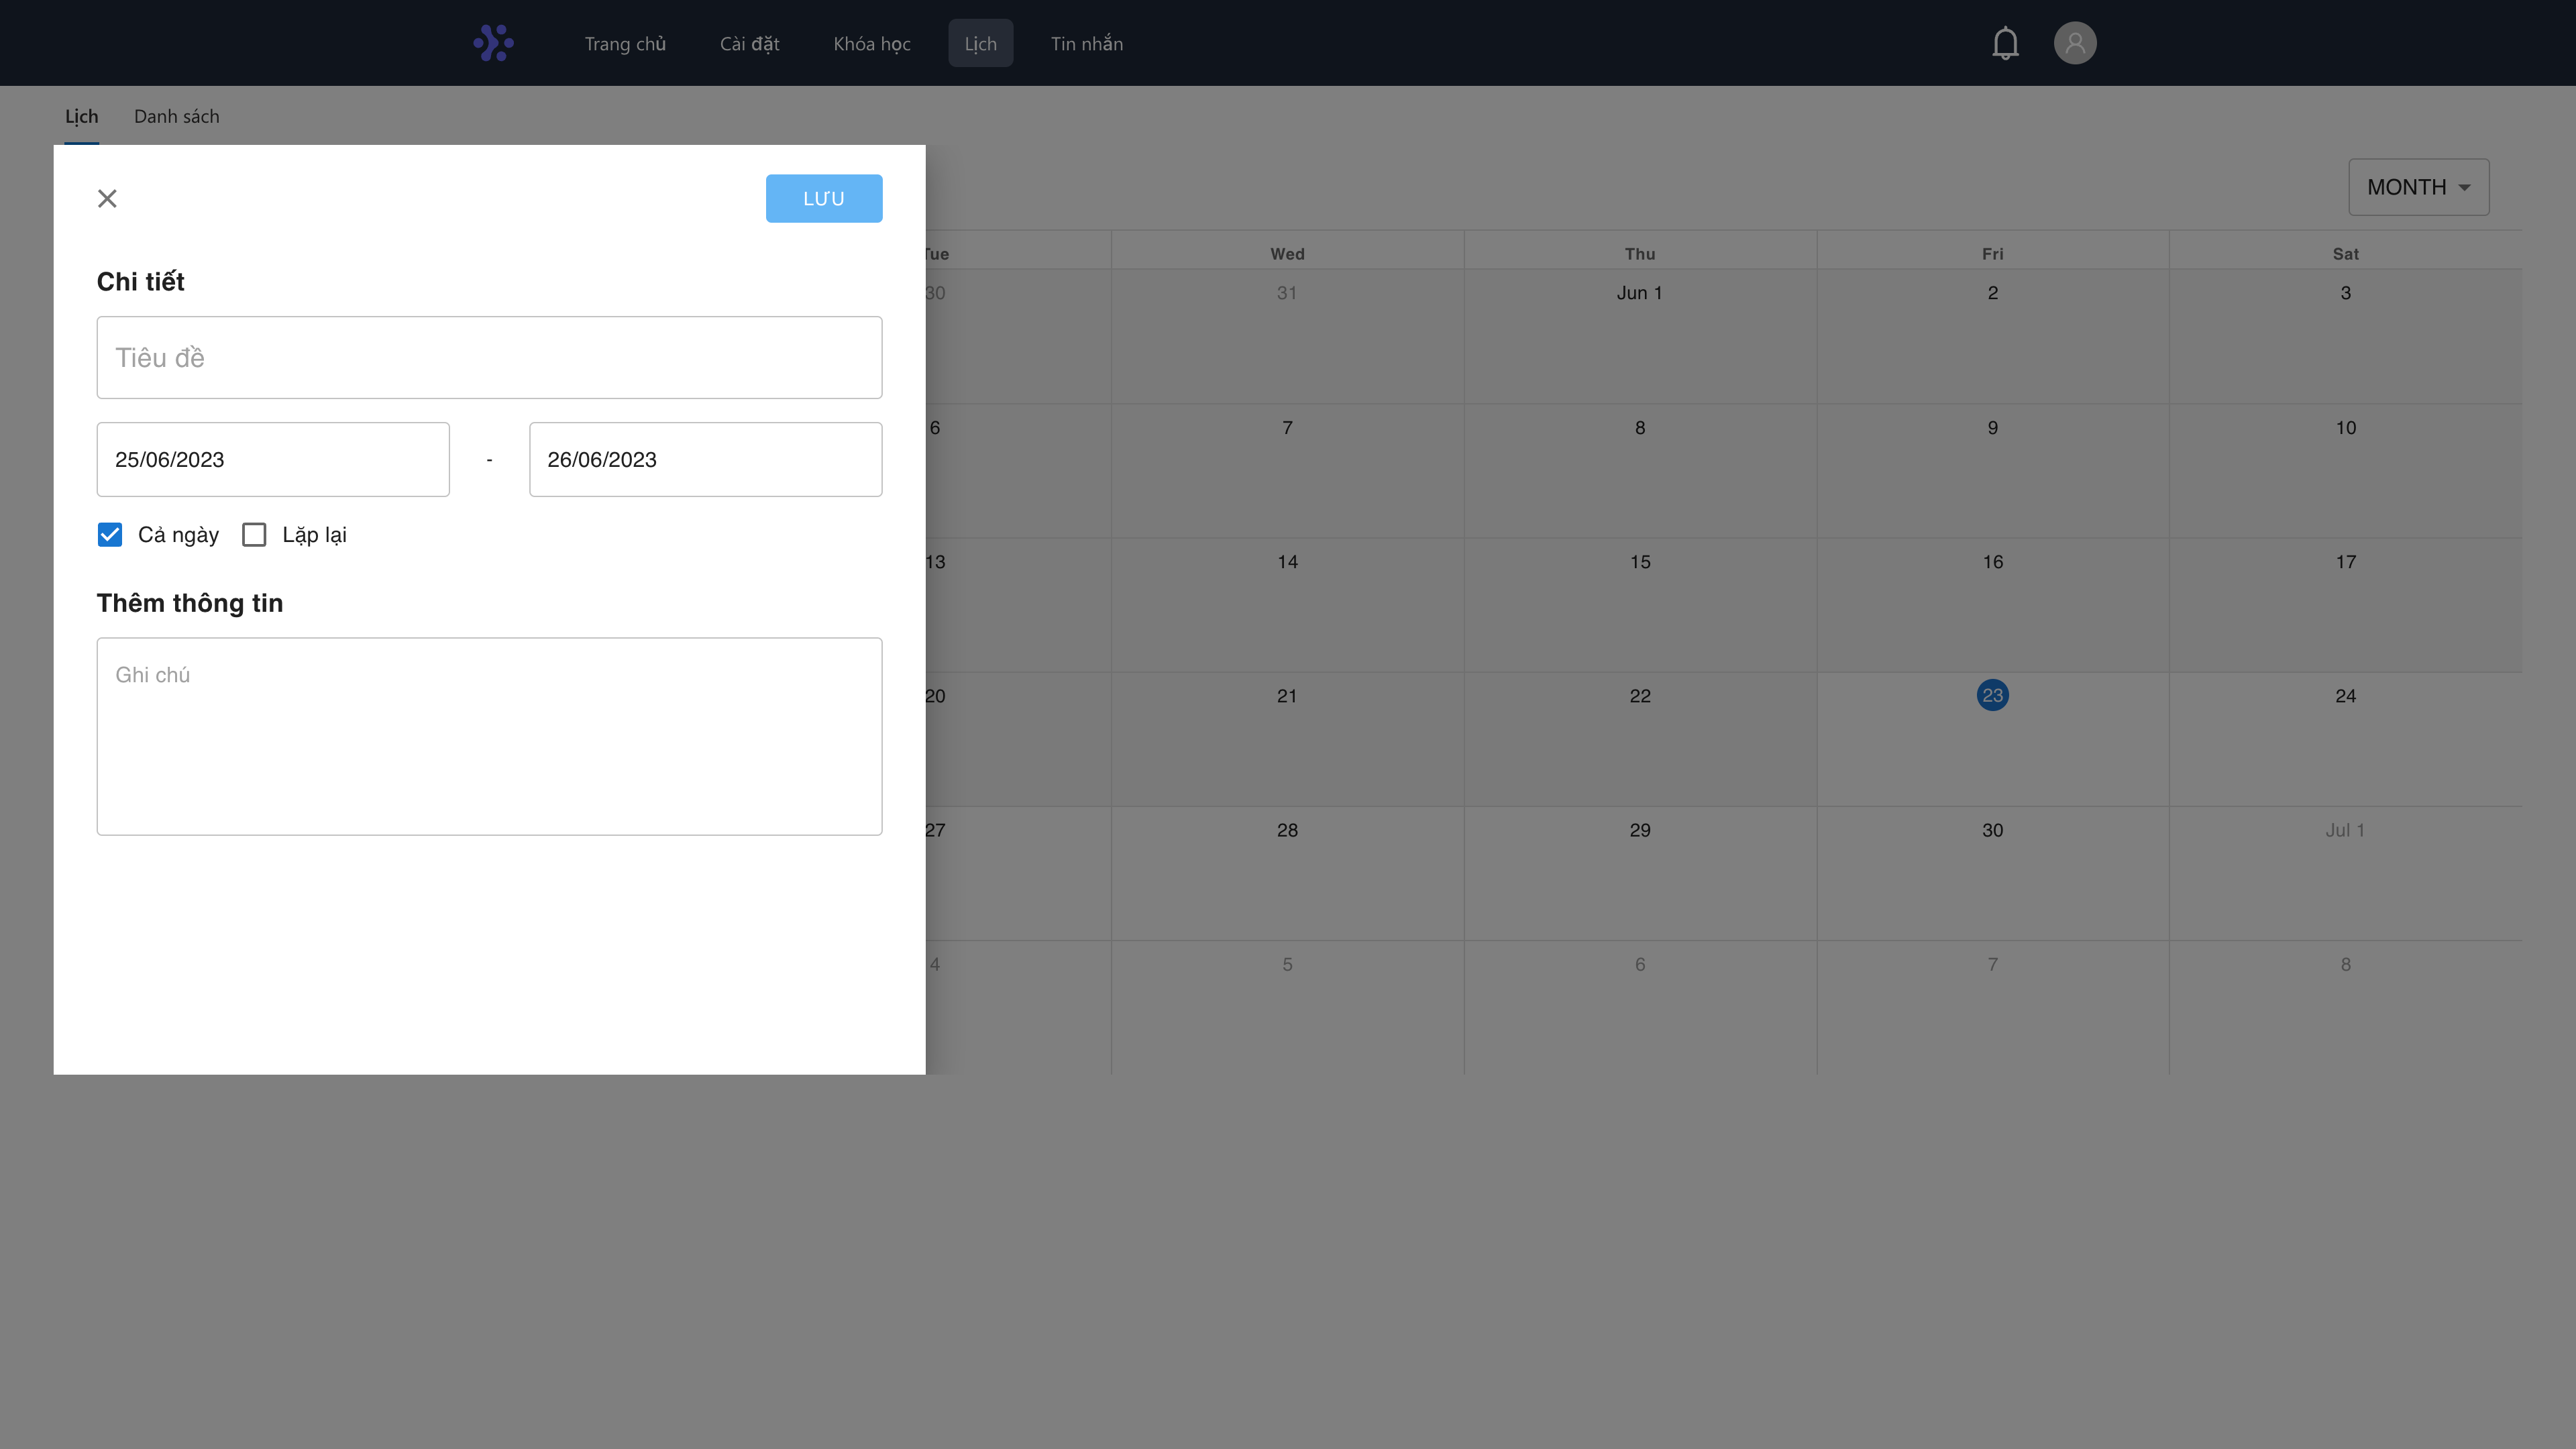
\includegraphics[width=300pt]{tao-su-kien}
            \caption{Màn hình tạo sự kiện của phần quản trị viên}
            \label{fig:tao-su-kien}
        \end{figure}


        Phần tin nhắn của phần quản trị viên được thể hiện ở hình:
        \begin{figure}[ht!]
            \centering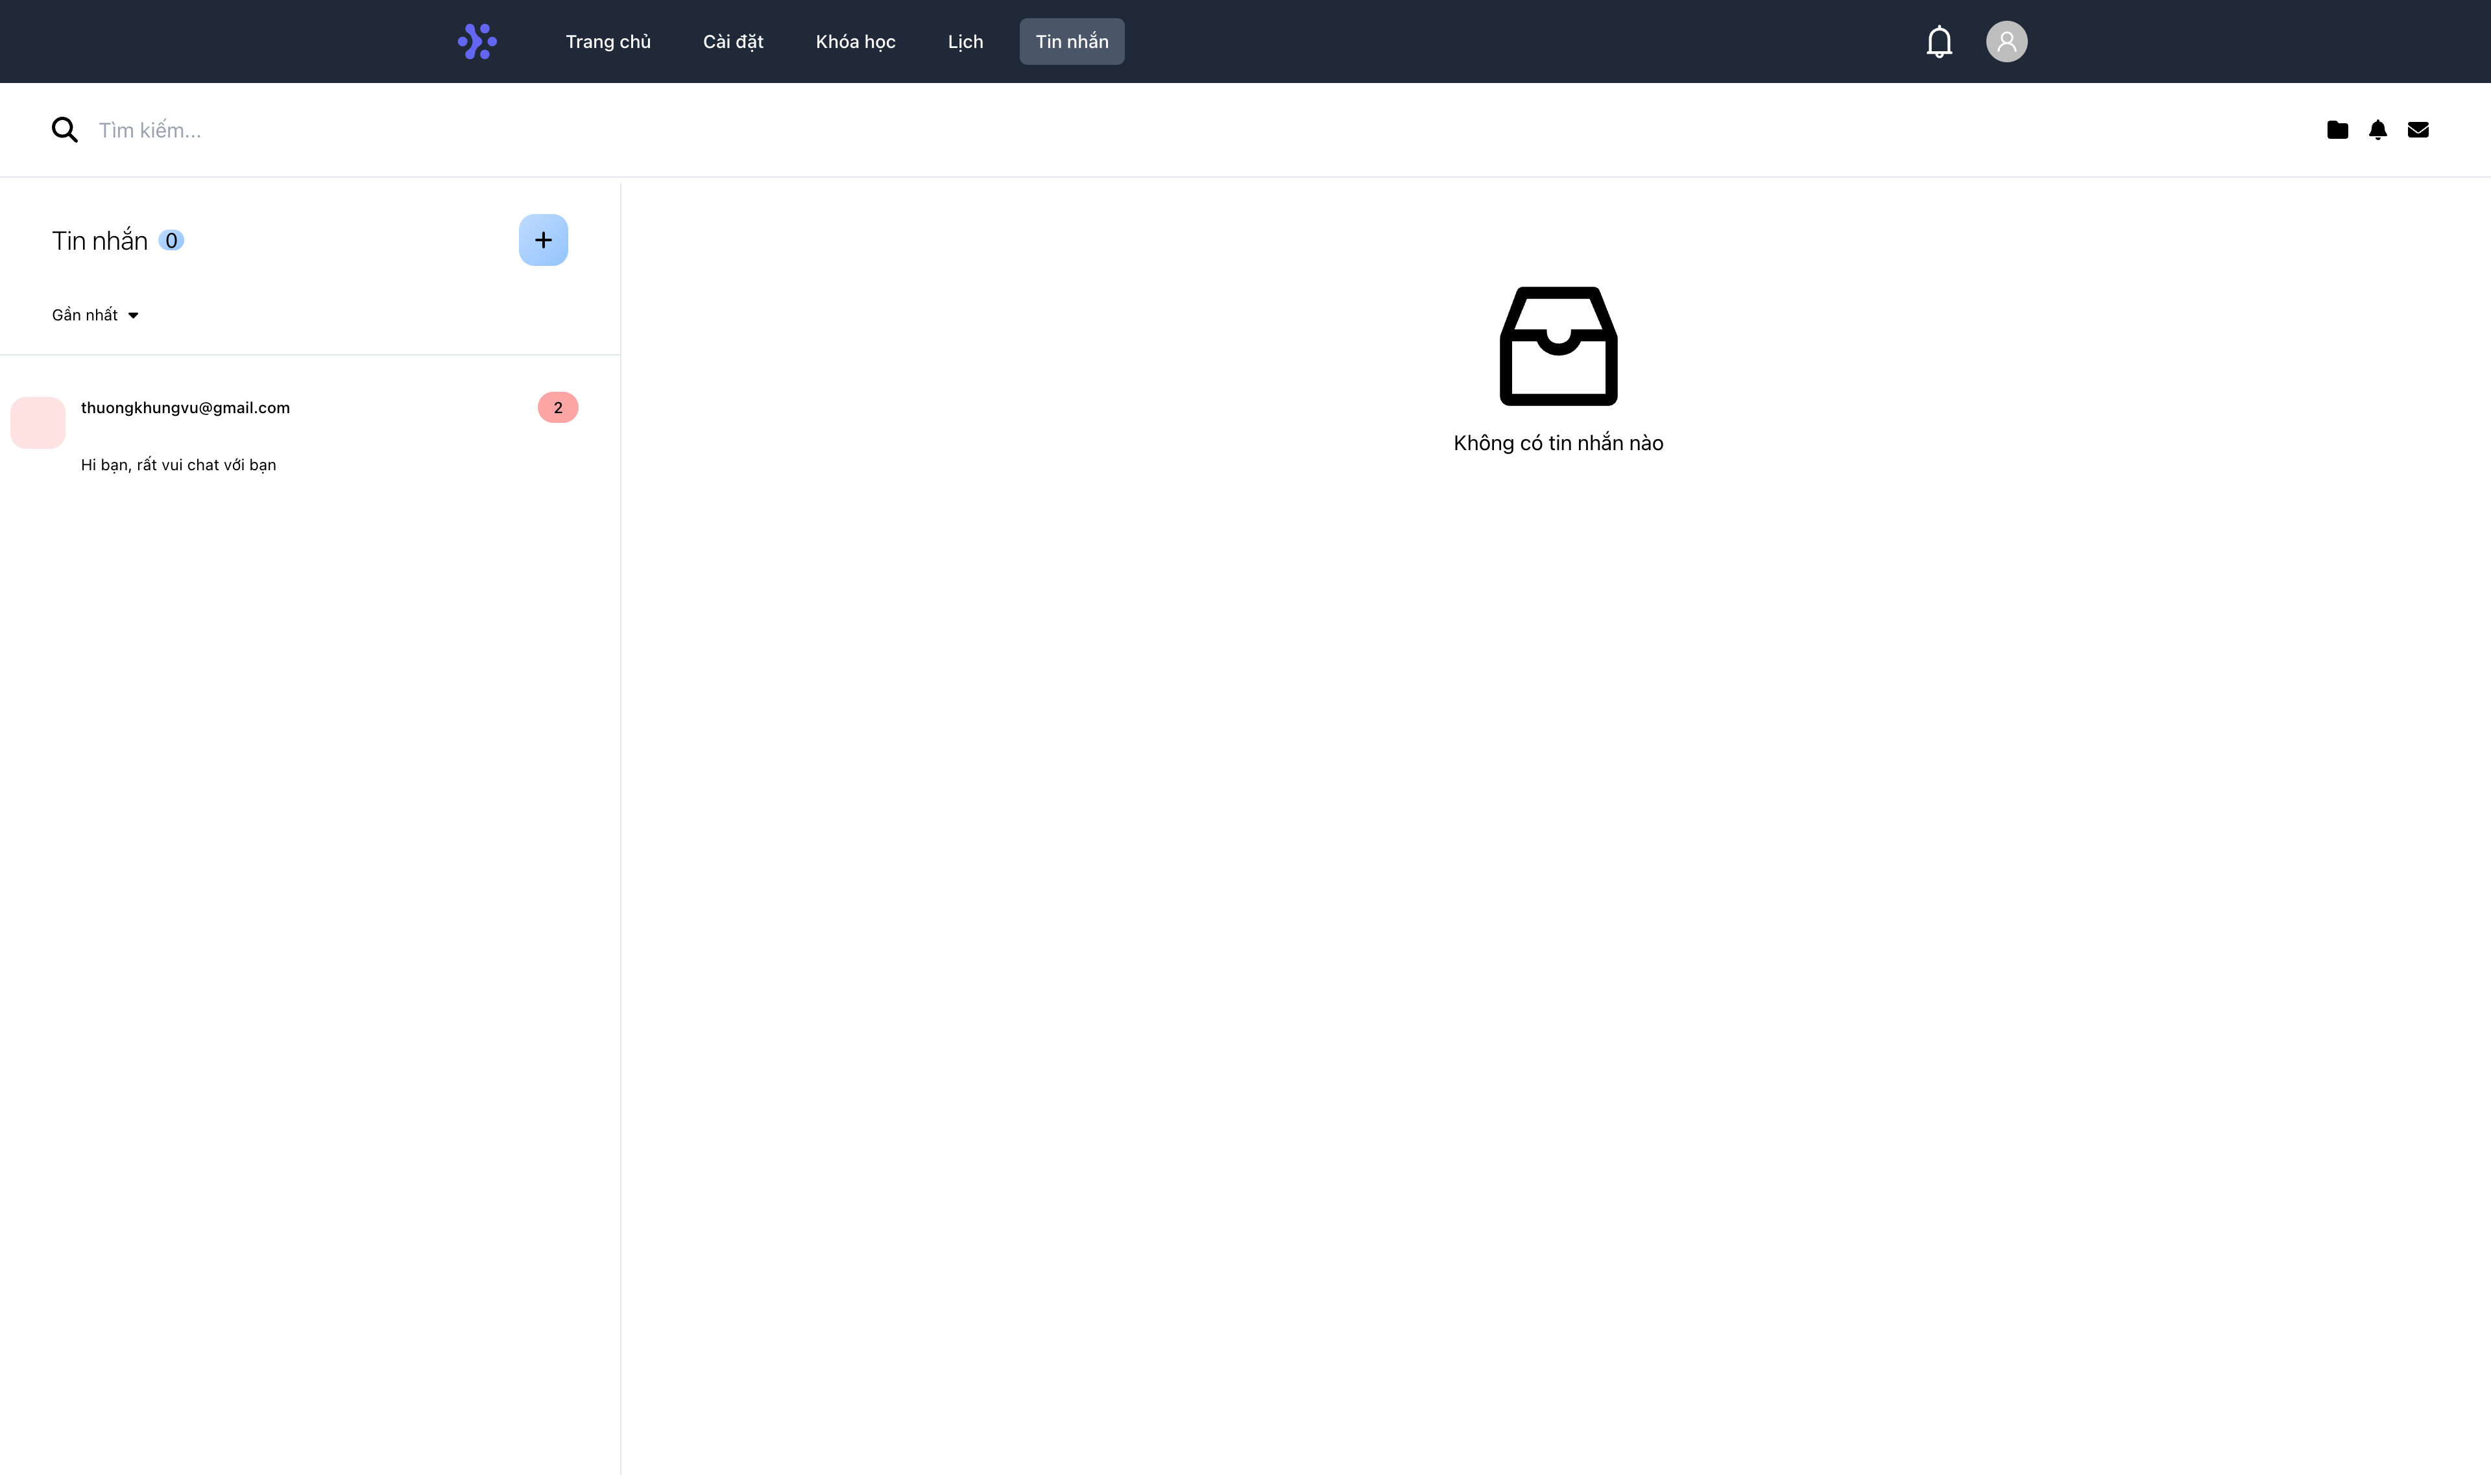
\includegraphics[width=300pt]{tin-nhan}
            \caption{Màn hình tin nhắn của phần quản trị viên}
            \label{fig:tin-nhan}
        \end{figure}

        Phần chi tiết tin nhắn của phần quản trị viên được thể hiện ở hình:
        \begin{figure}[ht!]
            \centering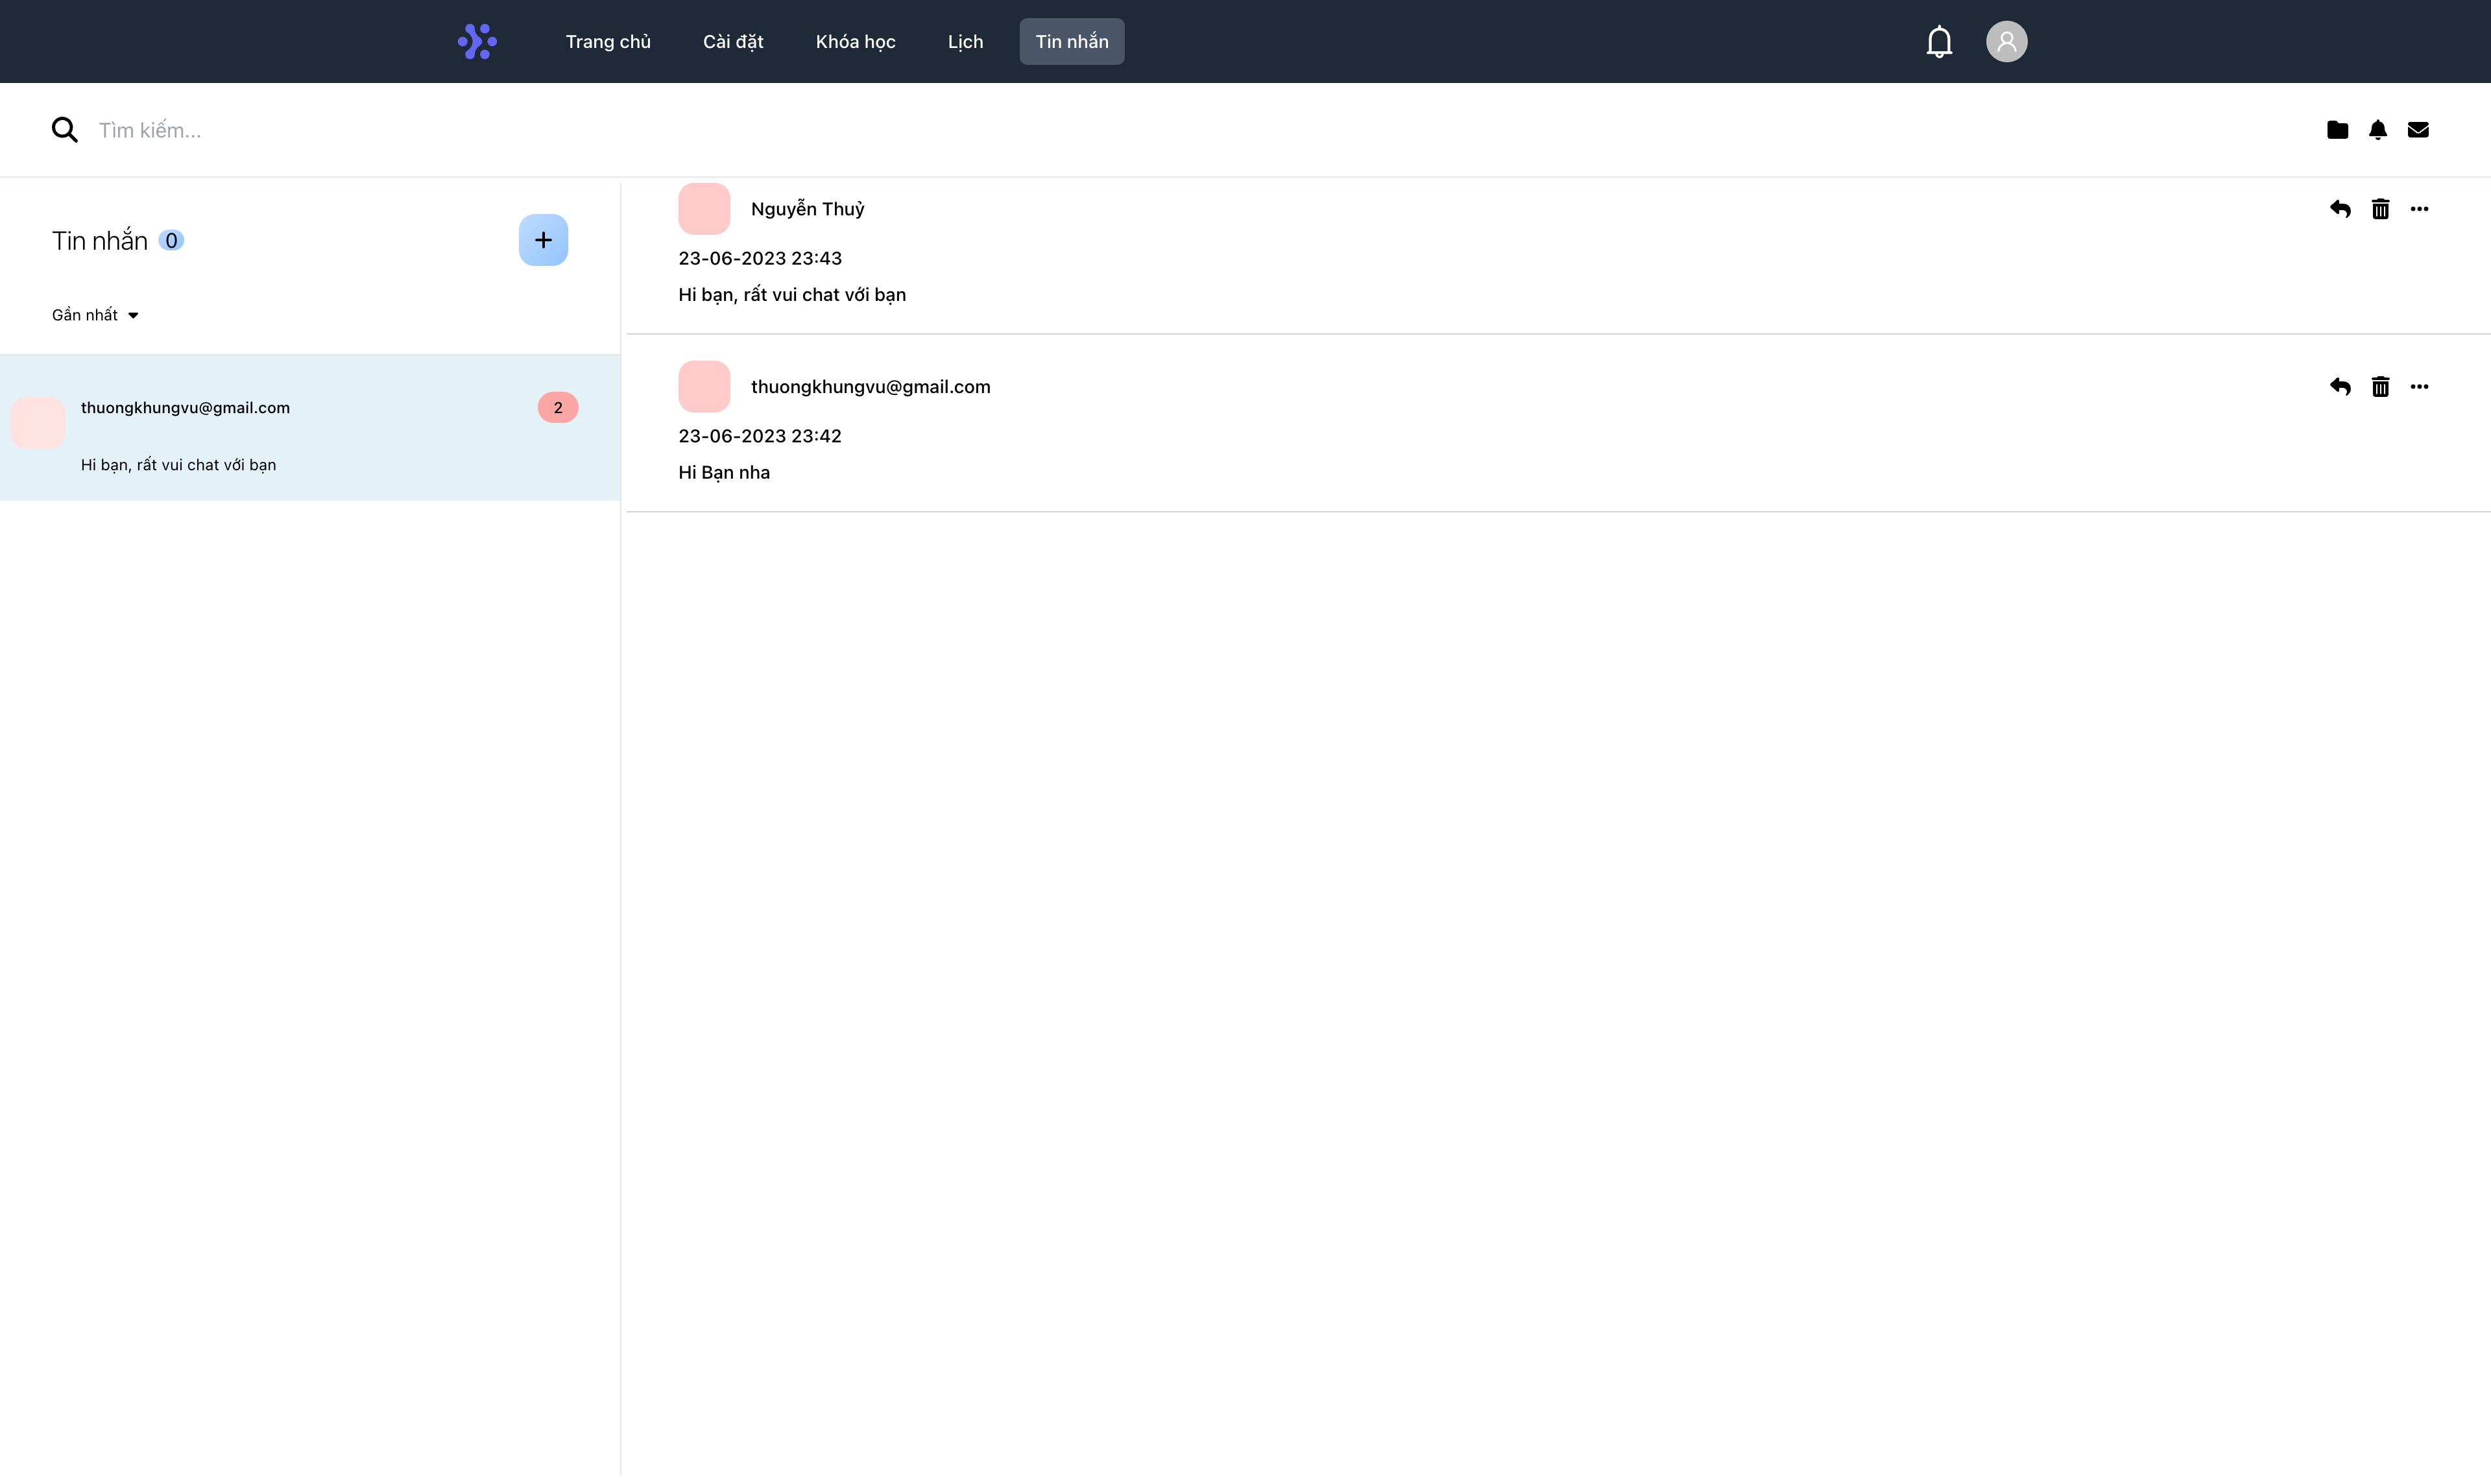
\includegraphics[width=300pt]{chi-tiet-tin-nhan}
            \caption{Màn hình chi tiết tin nhắn của phần quản trị viên}
            \label{fig:chi-tiet-tin-nhan}
        \end{figure}



\end{document}